
\documentclass[lang=cn,newtx,10pt,scheme=chinese]{elegantbook}
\title{角色动画入门}
\subtitle{Games105学习笔记}

\author{Sisyphes}
\institute{家里蹲}
\date{\today}
\version{0.9}
% \bioinfo{自定义}{信息}

% \extrainfo{使用的是优美的Elegant\LaTeX{} 模板}

\setcounter{tocdepth}{3}

\logo{logo-blue.png}
\cover{cover.jpg}

% 本文档命令
\usepackage{array}
\newcommand{\ccr}[1]{\makecell{{\color{#1}\rule{1cm}{1cm}}}}

% 修改标题页的橙色带
\definecolor{customcolor}{RGB}{32,178,170}
\colorlet{coverlinecolor}{customcolor}
\usepackage{cprotect}

\addbibresource[location=local]{reference.bib} % 参考文献,不要删除

\begin{document}

\maketitle
\frontmatter

\tableofcontents

\mainmatter

\chapter{0}
\section{废话}
写到最后,才是真的开始。目前有很多问题,后续看情况优化更新。

\chapter{角色动画介绍}

\begin{itemize}
  \item 模板官网:\href{https://elegantlatex.org/}{elegantlatex.org}
  \item 模板GitHub 地址:\href{https://github.com/ElegantLaTeX/}{ElegantLaTeX}
  \item 课程官网:\href{https://games-105.github.io/}{games-105}
  \item 课程Github 地址:\href{https://github.com/GAMES-105/GAMES-105}{GAMES-105-hw}
  \item 项目地址:\href{https://github.com/foocker}{Sisyphes}
  \item 作图工具:\href{https://www.geogebra.org/?lang=en}{geogebra}
\end{itemize}

\section{基本介绍}
这一节老师讲的比较精彩,建议看原视频,这里随便贴几张图。

\begin{figure}[htbp]
  \centering
  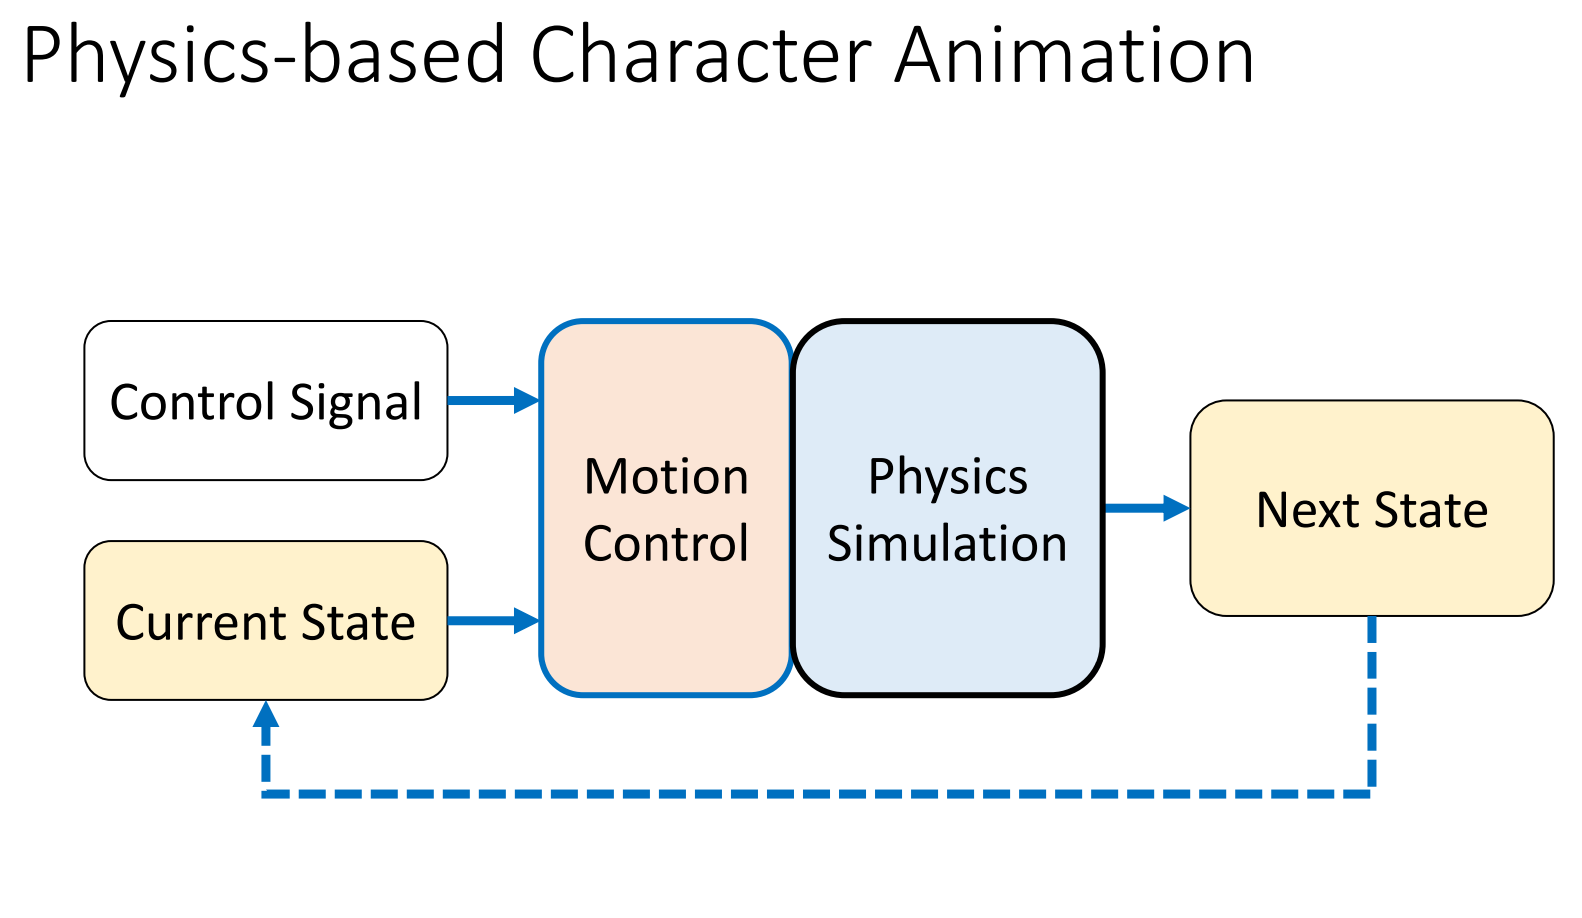
\includegraphics[totalheight=1.5in]{"./image/Physics-basedCharacterAnimation.png"}
  \caption{Physics-based Character Animation} \label{fig:Physics-basedCharacterAnimation}
\end{figure}

\begin{figure}[htbp]
  \centering
  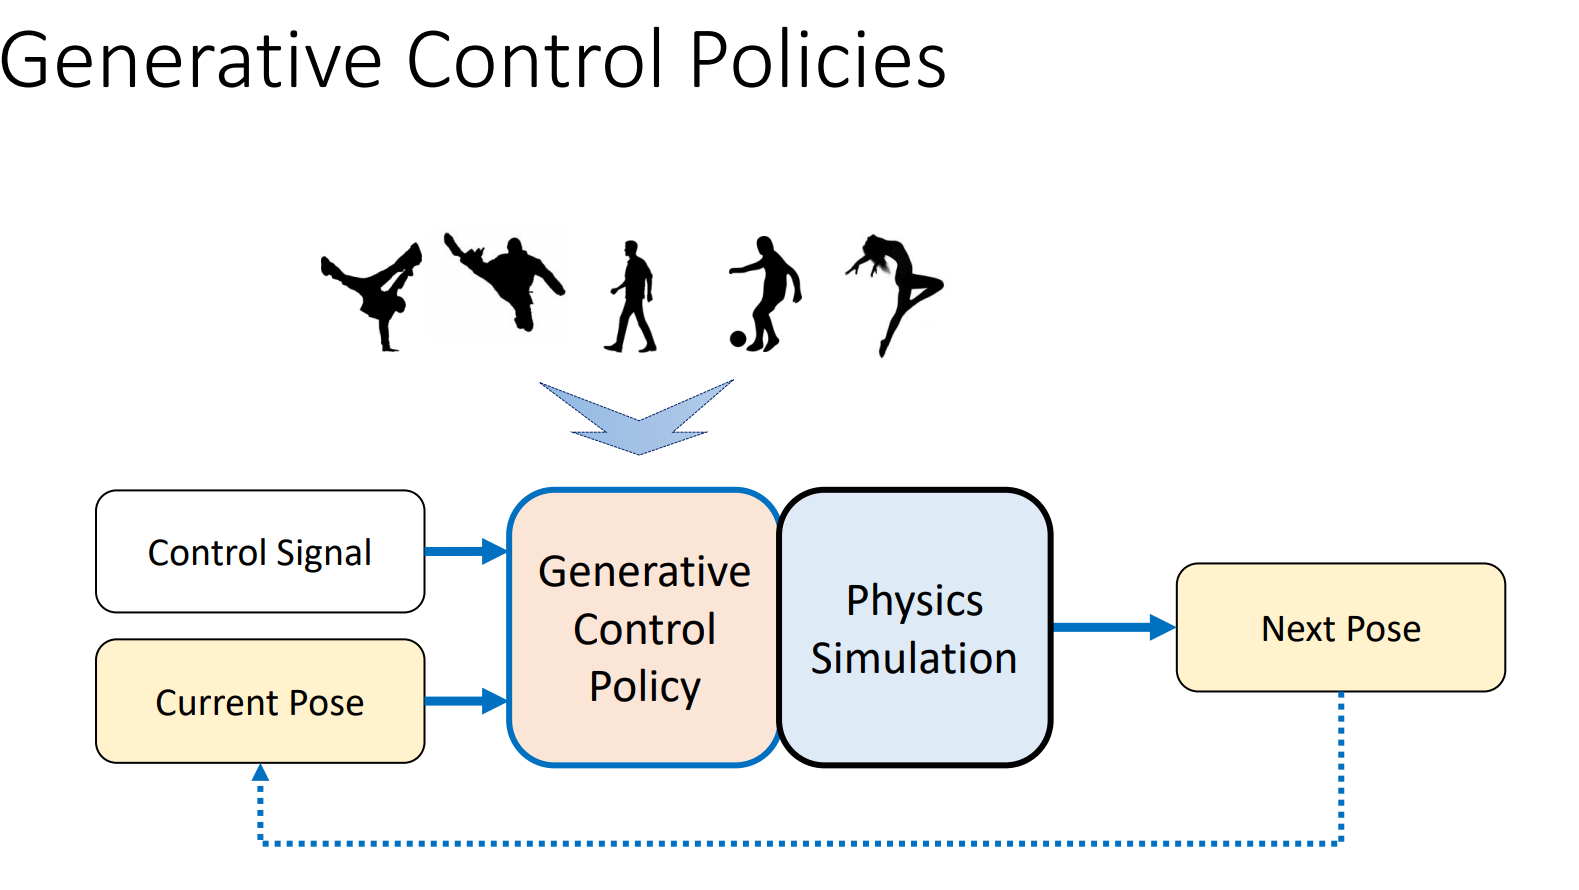
\includegraphics[totalheight=1.5in]{"./image/GenerativeControlPolicies.png"}
  \caption{Generative Control Policies} \label{fig:GenerativeControlPolicies}
\end{figure}

\begin{figure}[htbp]
  \centering
  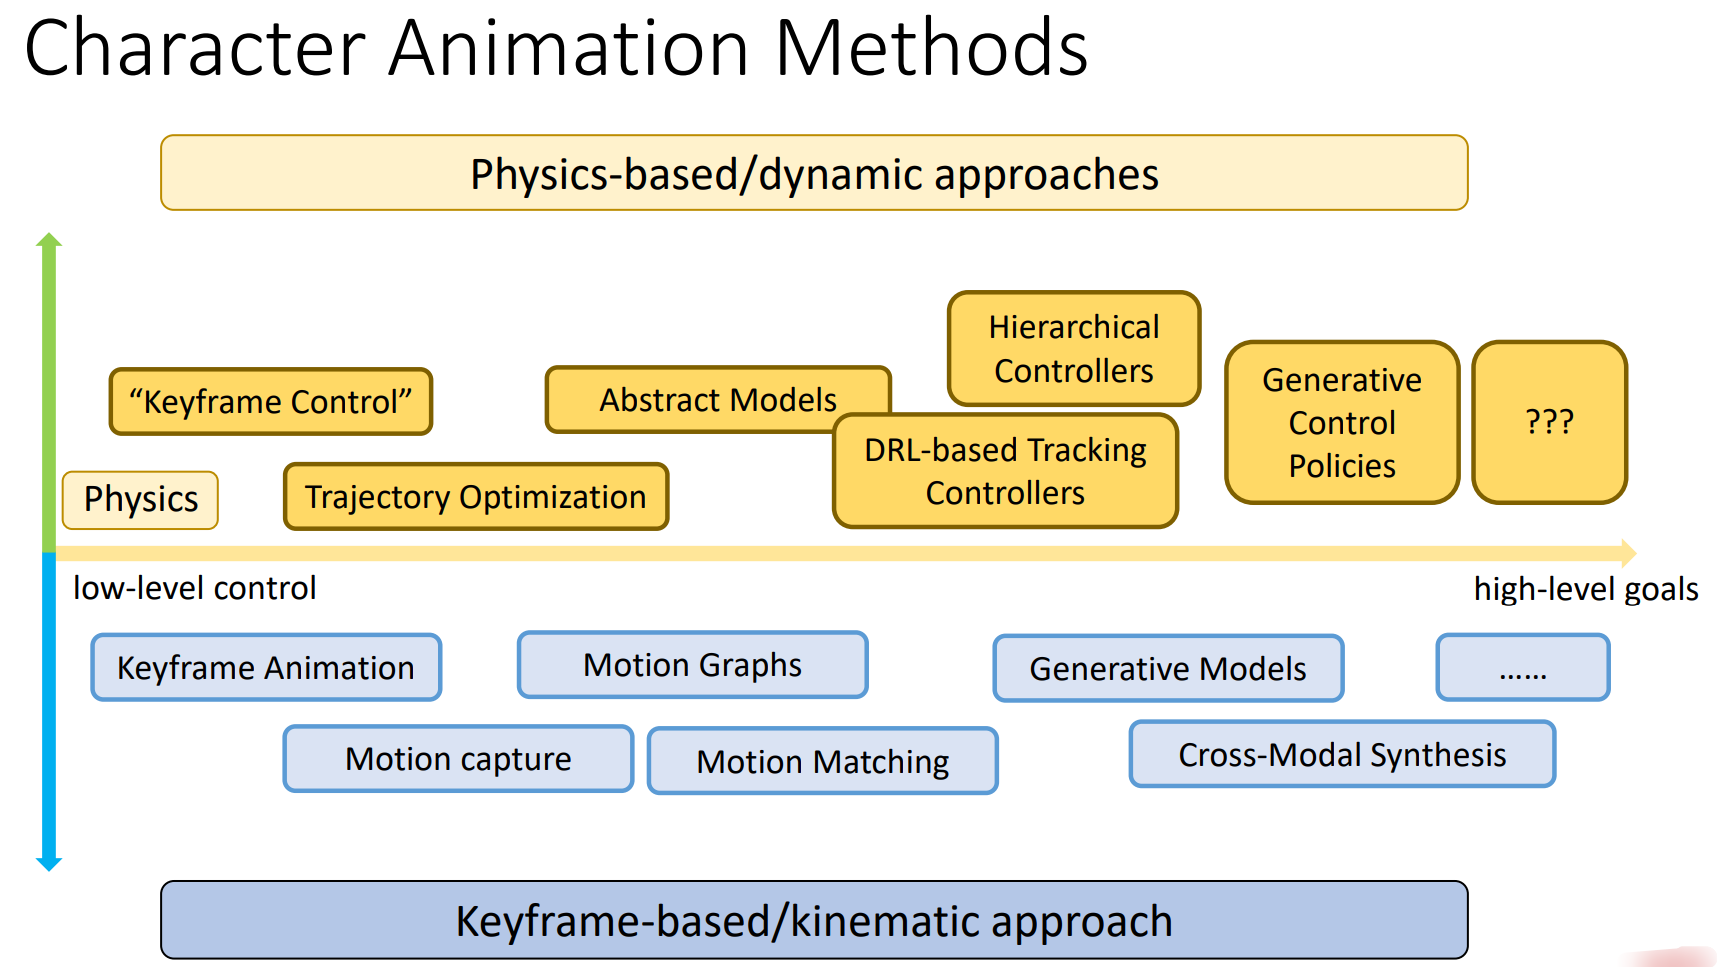
\includegraphics[totalheight=2in]{"./image/CharacterAnimationMethods.png"}
  \caption{Character Animation Methods} \label{fig:CharacterAnimationMethods}
\end{figure}


\section{工业应用与实践}
略。
\subsection{基础代码}
可参考\href{https://theorangeduck.com/page/all}{theorangeduck}等。
比如线性蒙皮LBS:
\begin{lstlisting}[language=C++]  
  // https://github.com/orangeduck/Motion-Matching/blob/main/character.h
  void linear_blend_skinning_positions(
    slice1d<vec3> anim_positions,
    const slice1d<vec3> rest_positions,
    const slice2d<float> bone_weights,
    const slice2d<unsigned short> bone_indices,
    const slice1d<vec3> bone_rest_positions,
    const slice1d<quat> bone_rest_rotations,
    const slice1d<vec3> bone_anim_positions,
    const slice1d<quat> bone_anim_rotations)
{
    anim_positions.zero();
    
    for (int i = 0; i < anim_positions.size; i++)
    {
        for (int j = 0; j < bone_indices.cols; j++)
        {
            if (bone_weights(i, j) > 0.0f)
            {
                int b = bone_indices(i, j);
                
                vec3 position = rest_positions(i);            
                position = quat_mul_vec3(quat_inv(bone_rest_rotations(b)), position - bone_rest_positions(b));
                position = quat_mul_vec3(bone_anim_rotations(b), position) + bone_anim_positions(b);
                
                anim_positions(i) = anim_positions(i) + bone_weights(i, j) * position;
            }
        } 
    }
}

void linear_blend_skinning_normals(
    slice1d<vec3> anim_normals,
    const slice1d<vec3> rest_normals,
    const slice2d<float> bone_weights,
    const slice2d<unsigned short> bone_indices,
    const slice1d<quat> bone_rest_rotations,
    const slice1d<quat> bone_anim_rotations)
{
    anim_normals.zero();
    
    for (int i = 0; i < anim_normals.size; i++)
    { 
        for (int j = 0; j < bone_indices.cols; j++)
        {
            if (bone_weights(i, j) > 0.0f)
            {
                int b = bone_indices(i, j);
                
                vec3 normal = rest_normals(i);
                normal = quat_mul_vec3(quat_inv(bone_rest_rotations(b)), normal);
                normal = quat_mul_vec3(bone_anim_rotations(b), normal);
                
                anim_normals(i) = anim_normals(i) + bone_weights(i, j) * normal;
            }
        }
    }
    
    for (int i = 0; i < anim_normals.size; i++)
    { 
        anim_normals(i) = normalize(anim_normals(i));
    }
}

\end{lstlisting}

比如运动学中的前后向驱动:
\begin{lstlisting}[language=C++]  % 前向运动FK
// https://github.com/orangeduck/Animation-Looping/blob/main/database.h
// Here I am using a simple recursive version of forward kinematics
void forward_kinematics(
    vec3& bone_position,
    quat& bone_rotation,
    const slice1d<vec3> bone_positions,
    const slice1d<quat> bone_rotations,
    const slice1d<int> bone_parents,
    const int bone)
{
    if (bone_parents(bone) != -1)
    {
        vec3 parent_position;
        quat parent_rotation;
        
        forward_kinematics(
            parent_position,
            parent_rotation,
            bone_positions,
            bone_rotations,
            bone_parents,
            bone_parents(bone));
        
        bone_position = quat_mul_vec3(parent_rotation, bone_positions(bone)) + parent_position;
        bone_rotation = quat_mul(parent_rotation, bone_rotations(bone));
    }
    else
    {
        bone_position = bone_positions(bone);
        bone_rotation = bone_rotations(bone); 
    }
}
\end{lstlisting}

\begin{lstlisting}[language=C++]  % 反向运动IK
// https://github.com/orangeduck/Animation-Looping/blob/main/database.h
// Compute backward kinematics for all joints
void backward_kinematics_full(
    slice1d<vec3> local_bone_positions,
    slice1d<quat> local_bone_rotations,
    const slice1d<vec3> global_bone_positions,
    const slice1d<quat> global_bone_rotations,
    const slice1d<int> bone_parents)
{
    for (int i = 0; i < bone_parents.size; i++)
    {
        if (bone_parents(i) == -1)
        {
            local_bone_positions(i) = global_bone_positions(i);
            local_bone_rotations(i) = global_bone_rotations(i);
        }
        else
        {
            vec3 parent_position = global_bone_positions(bone_parents(i));
            quat parent_rotation = global_bone_rotations(bone_parents(i));

            local_bone_positions(i) = quat_inv_mul_vec3(parent_rotation,
                global_bone_positions(i) - parent_position);
            local_bone_rotations(i) = quat_inv_mul(parent_rotation, global_bone_rotations(i));
        }
    }
}
\end{lstlisting}

\section{学术进展}
\begin{enumerate}
  \item \href{https://www.zhihu.com/column/c_1061982920763293696}{角色动画论文选读}
  \item \href{https://github.com/rosswhitfield/ase}{ASE}
  \item 作者团队新论文\href{https://github.com/heyuanYao-pku/Control-VAE}{Control-VAE}\
  \item DL代码更新汇集\href{https://github.com/sebastianstarke/AI4Animation}{AI4Animation}
  \item \href{https://github.com/orangeduck/Motion-Matching}{Motion-Matching}
  \item \href{https://theorangeduck.com/page/code-vs-data-driven-displacement}{code-vs-data-driven-displacement}
\end{enumerate}

\chapter{数学基础}

由向量点乘定义:$\mathbf{ab}=\lVert \mathbf{a} \rVert  \lVert \mathbf{b} \rVert \cos(\theta)$,得到
向量$\mathbf{a}$在向量$\mathbf{b}$上的投影:$\mathbf{a}_\mathbf{b} = \lVert \mathbf{a} 
\rVert \cos(\theta) = \frac{\mathbf{ab}}{\lVert \mathbf{b} \rVert}$

叉乘

\begin{equation}
  \begin{aligned}
  \boldsymbol{c}=\boldsymbol{a} \times \boldsymbol{b} & =\left[\begin{array}{c}
  a_y b_z-a_z b_y \\
  a_z b_x-a_x b_z \\
  a_x b_y-a_y b_x
  \end{array}\right] \\
  & =\left[\begin{array}{ccc}
  0 & -a_z & a_y \\
  a_z & 0 & -a_x \\
  -a_y & a_x & 0
  \end{array}\right]\left[\begin{array}{l}
  b_x \\
  b_y \\
  b_z
  \end{array}\right]=[\boldsymbol{a}]_{\times} \boldsymbol{b}\\
  &=\|\boldsymbol{a}\|\boldsymbol{b}\| \sin (\theta) \boldsymbol{n}\\
  &=det\left[\begin{array}{ccc}
    \boldsymbol{i} & \boldsymbol{j} & \boldsymbol{k} \\
    a_x & a_y & a_z \\
    b_x & b_y & b_z
    \end{array}\right]
  \end{aligned}
\end{equation}

其中\(\boldsymbol{n}\)是由 $\boldsymbol{a}$ 到$\boldsymbol{b}$在右手坐标系
下的第三个方向的方向向量,$[\boldsymbol{a}]_{\times}$表示$\boldsymbol{a}$的
叉乘矩阵,注意是一个叉乘对应一个矩阵写法,比如$(\boldsymbol{a} \times \boldsymbol{b}) \times \boldsymbol{c}=[\boldsymbol{a} \times \boldsymbol{b}]_{\times} \boldsymbol{c}$
另外,两向量的叉乘其叉乘矩阵是一个反对称阵。

点积和叉积的一个典型应用是确定两向量的最小旋转角。将一个向量旋转到另一个向量,
沿着两向量叉乘后的方向向量旋转点积的运算得到的余弦角度。

向量的旋转:向量$\boldsymbol{a}$沿着向量$\boldsymbol{u}$旋转
$\theta$得到$\boldsymbol{b}$,如何计算$\boldsymbol{b}$。
具体推到见图:$\boldsymbol{b} = \boldsymbol{a} + \boldsymbol{v} + \boldsymbol{t}$,
$\boldsymbol{v} = (\sin(\theta))\boldsymbol{u} \times \boldsymbol{a}$,
$\boldsymbol{t} = (1 - \cos(\theta))\boldsymbol{u} \times (\boldsymbol{u} \times \boldsymbol{a})$

% \begin{minipage}
  
% \end{minipage}
Rodrigues'旋转公式:
\begin{equation}
  \boldsymbol{b}= \boldsymbol{a}+(\sin \theta) \boldsymbol{u} \times \boldsymbol{a}+(1-\cos \theta) \boldsymbol{u} \times(\boldsymbol{u} \times \boldsymbol{a})
\end{equation}

由正交基的写法$\boldsymbol{a} = a_x \boldsymbol{e_x} + 
                  a_y \boldsymbol{e_y} +
                  a_z \boldsymbol{e_z}$
可以得到点乘和叉乘的公式。

单位阵,对角阵,对称阵,反(skew)对称阵 $A^T = -A,[\boldsymbol{a}]_{\times}+[\boldsymbol{a}]^{T}_{\times}=\boldsymbol{0} $,
正交阵,$A^{T}A=I, det(A)=\pm 1$,特征值,特征向量 $A\boldsymbol{x}=\lambda\boldsymbol{x}$。

这里默认向量是列向量。因此$\boldsymbol{a}\boldsymbol{b}=\boldsymbol{a^T b}=
\boldsymbol{b^{T}a}$,同时

有了叉乘矩阵的写法,可以将Rodrigues'公式用矩阵形式重写。

行列式的基本性质:
\begin{itemize}
  \setlength{\itemindent}{2em}
  \item $det I = 1$
  \item $det AB = det A * det B $
  \item $det A^T = det A$
  \item 可逆:$det A^{-1} = (det A)^{-1}$
  \item 正交:$det U = \pm 1$
\end{itemize}

\section{刚体变换}
平移,旋转,缩放,仿射变换。

旋转矩阵行列式为1,所以不会改变坐标轴的顺序,同时$R\boldsymbol{u}=\boldsymbol{u}=R^{T}\boldsymbol{u}$
得到$(R-R^T)\boldsymbol{u}=0$,因为$R-R^T$是一个反对称阵,可将其写为
叉乘形式,$\boldsymbol{u^{'}}\times \boldsymbol{u}=0$,其中$\boldsymbol{u^{'}}$
一般非0。当旋转矩阵是对称阵是,比如绕$\boldsymbol{u^{'}}$轴旋转$k\pi$度。
由Rodrigues'公式
\begin{equation}
  R=I+(\sin \theta)[\boldsymbol{u}]_{\times}+(1-\cos \theta)[\boldsymbol{u}]_{\times}^2
\end{equation}
得到
\begin{equation}
  \boldsymbol{u} \leftarrow \boldsymbol{u}^{\prime}=\left[\begin{array}{l}
  r_{32}-r_{23} \\
  r_{13}-r_{31} \\
  r_{21}-r_{12}
  \end{array}\right] \leftarrow R-R^{\mathrm{T}}
\end{equation}
进一步得到旋转轴的长度
$\|\boldsymbol{u^{'}}=2\sin(\theta)$。

\subsection{坐标系变换}
物体坐标系的坐标不因旋转的改变而改变,而旋转本身会改变其在世界坐标系
下的坐标表示,对于同一点$\boldsymbol{a}$,其旋转前后有如下关系:
$\left(x^{\prime}, y^{\prime}, z^{\prime}\right)^T: 
\boldsymbol{a}$ 在物体坐标系中 $(x, y, z)^T: 
\boldsymbol{a}$ 在全局坐标系中
$$
\begin{aligned}
\boldsymbol{a} & =\left[\begin{array}{ccc}
1 & \mid & \mid \\
\boldsymbol{e}_x & \boldsymbol{e}_y & \boldsymbol{e}_z \\
\mid & \mid & \mid
\end{array}\right]\left[\begin{array}{l}
x \\
y \\
z
\end{array}\right] \\
& =\left[\begin{array}{ccc}
\mid & \mid & \mid \\
\boldsymbol{e}_x^{\prime} & \boldsymbol{e}_y^{\prime} & \boldsymbol{e}_z^{\prime} \\
\mid & \mid & \mid
\end{array}\right]\left[\begin{array}{l}
x^{\prime} \\
y^{\prime} \\
z^{\prime}
\end{array}\right]
\end{aligned}
$$
因此旋转矩阵表示为将局部坐标映射为全局坐标的变换矩阵。
\begin{equation}
  \begin{gathered}
  R=\left[\begin{array}{ccc}
  \mid & \mid & \mid \\
  \boldsymbol{e}_x & \boldsymbol{e}_y & \boldsymbol{e}_z \\
  \mid & \mid & \mid
  \end{array}\right]^{-1}\left[\begin{array}{ccc}
  \mid & \mid & \mid \\
  \boldsymbol{e}_x^{\prime} & \boldsymbol{e}_y^{\prime} & \boldsymbol{e}_z^{\prime} \\
  \mid & \mid & \mid
  \end{array}\right] \\
  {\left[\begin{array}{l}
  x \\
  y \\
  z
  \end{array}\right]=R\left[\begin{array}{l}
  x^{\prime} \\
  y^{\prime} \\
  z^{\prime}
  \end{array}\right]}
  \end{gathered}
\end{equation}

当存在平移时,从物体坐标到全局坐标有:
\begin{equation}
  \left[\begin{array}{l}
    x \\
    y \\
    z
  \end{array}\right]
  =R\left[\begin{array}{l}
    x^{\prime} \\
    y^{\prime} \\
    z^{\prime}
    \end{array}\right] + \boldsymbol{t}
\end{equation}
从全局坐标到物体坐标:
\begin{equation}
  \left[\begin{array}{l}
    x^{\prime} \\
    y^{\prime} \\
    z^{\prime}
  \end{array}\right]
  =R^{T}\left(\left[\begin{array}{l}
    x \\
    y \\
    z
    \end{array}\right] - \boldsymbol{t} \right)
\end{equation}
正交阵的自由度是3。

绕坐标轴的旋转矩阵:
\begin{equation}
  \begin{aligned}
  & R_x(\alpha)=\left(\begin{array}{ccc}
  1 & 0 & 0 \\
  0 & \cos \alpha & -\sin \alpha \\
  0 & \sin \alpha & \cos \alpha
  \end{array}\right) \\
  & R_y(\beta)=\left(\begin{array}{ccc}
  \cos \beta & 0 & \sin \beta \\
  0 & 1 & 0 \\
  -\sin \beta & 0 & \cos \beta
  \end{array}\right) \\
  & R_z(\gamma)=\left(\begin{array}{ccc}
  \cos \gamma & -\sin \gamma & 0 \\
  \sin \gamma & \cos \gamma & 0 \\
  0 & 0 & 1
  \end{array}\right)
  \end{aligned}
\end{equation}

任何旋转都可以由沿基本轴的旋转合成。需要注意的是,分别沿$x,y,z$轴
旋转$\alpha, \beta, \gamma$时,基本轴选择物体坐标系时,其旋转矩阵(Intrinsic)为
$R_x(\alpha)R_y(\beta)R_z(\gamma)$,基本轴旋转世界坐标系时,旋转矩阵(Extrinsic)为
$R_z(\gamma)R_y(\beta)R_x(\alpha)$。常见工具maya是物体坐标系,Unity是可选择,
但基本顺序是YXZ。

平移插值:$x_t = (1-t)x_0 + x_t$。

旋转插值:矩阵形式几乎无法操作;欧拉角表示做多次矩阵乘法,同时
需要处理奇点($\alpha+n\pi$)问题,比如人在原地转圈,万向锁问题等;
轴角表示($u, \theta$),做旋转组合比较麻烦,常见插值$\theta_t=(1-t)\theta_0 + \theta_1$ 。
其旋转速度不恒定,恒定方式为:\begin{equation}
  \begin{aligned}
  R(\delta \boldsymbol{\theta}) & =R^T\left(\boldsymbol{\theta}_0\right) R\left(\boldsymbol{\theta}_1\right) \\
  \delta \boldsymbol{\theta}_t & =(1-t) \mathbf{0}+t \delta \boldsymbol{\theta} \\
  R\left(\boldsymbol{\theta}_t\right) & =R\left(\boldsymbol{\theta}_0\right) R\left(\delta \boldsymbol{\theta}_t\right)
  \end{aligned}
\end{equation}
四元数表示(2D旋转可由复数表示,3D旋转最终由William Rowan Hamilton发明了四元数解决),
\begin{equation}
  \label{WilliamRowanHamilton}
  \begin{aligned}
  \boldsymbol{q}_{\boldsymbol{t}} & =\frac{\sin [(1-t) \theta]}{\sin \theta} \boldsymbol{q}_0+\frac{\sin t \theta}{\sin \theta} \boldsymbol{q}_1 \\
  & cos \theta  = \boldsymbol{q}_0 \boldsymbol{q}_1
  \end{aligned}
\end{equation}

\subsection{四元数}
基本定义,基本性质(加减乘除点积,共轭,范数,矩阵表示等)参考\href{https://en.wikipedia.org/wiki/Quaternion}{Quaternion}。

四元数(quaternion)的矩阵记法:
$\boldsymbol{q} = w + x\boldsymbol{i} + y\boldsymbol{j} + z\boldsymbol{k}=
\left[\begin{array}{l}
  w \\
  x \\
  y \\
  z
  \end{array}\right]
= 
\left[\begin{array}{l}
  w \\
  \boldsymbol{v}
  \end{array}\right]
  $

扩展定义:
$q=[w, \boldsymbol{v}]^{\mathrm{T}} \in \mathbb{H}, w \in \mathbb{R}, 
\boldsymbol{v} \in \mathbb{R}^3$。
$w=[w, \mathbf{0}]^{\mathrm{T}}$ : 常量四元数。
$\boldsymbol{v}=[0, \boldsymbol{v}]^{\mathrm{T}}:$ 纯四元数。
记法
$
\left[\begin{array}{l}
  w \\
  \boldsymbol{v}
  \end{array}\right]
  $
容易写出其基本运算规律,比如$\boldsymbol{q}^{*}=[w, -\boldsymbol{v}]^T$,
乘法\begin{equation}
  \boldsymbol{q}_1 \boldsymbol{q}_{\mathbf{2}}=\left[\begin{array}{l}
  w_1 \\
  \boldsymbol{v}_{\mathbf{1}}
  \end{array}\right]\left[\begin{array}{c}
  w_2 \\
  \boldsymbol{v}_{\mathbf{2}}
  \end{array}\right]=\left[\begin{array}{c}
  w_1 w_2-\boldsymbol{v}_1 \cdot \boldsymbol{v}_2 \\
  w_1 \boldsymbol{v}_2+w_2 \boldsymbol{v}_1+\boldsymbol{v}_1 \times \boldsymbol{v}_2
  \end{array}\right]
  \end{equation}
有基本性质:
\begin{itemize}
  \item 共轭$(\boldsymbol{q}_1 \boldsymbol{q}_2)^*
  = \boldsymbol{q}^{*}_2 \boldsymbol{q}^{*}_1$
  \item 范数 $\|q\|^2 = q^{*}q= qq^{*}$
  \item 逆 $qq^{-1}=1 \rightarrow q^{-1}=\frac{q^*}{\|q\|^2}$
  \item 单位四元数 $\|q\|=1, q^{-1}=q^*=
  \left[\begin{array}{l}
    w \\
    \boldsymbol{v}
    \end{array}\right] \Leftrightarrow R^{-1} = R^T$
\end{itemize}

对比复平面上单位圆的表示,单位四元数可表示为4D空间中的超球面上的
点,$\left[\begin{array}{l}
  \cos\frac{\theta}{2}, \\
  \boldsymbol{u}\sin\frac{\theta}{2} 
  \end{array}\right], \|\boldsymbol{u}\|=1$。
表示的含义和轴角表示相同$(\boldsymbol{u}, \theta)$。
具体而言,任何3D旋转$(\boldsymbol{v}, \theta)$的单位四元数表示为
$
\left[\begin{array}{l}
  w \\
  \boldsymbol{v}
\end{array}\right] = \left[ \cos\frac{\theta}{2}, 
\boldsymbol{u}\sin\frac{\theta}{2} \right]
$
其轴角表示的
角度$\theta = 2 arg \cos w$,轴为$\boldsymbol{u}=
\frac{\boldsymbol{v}}{\|\boldsymbol{v}\|}$。
这里左右表达在行列上有差异,右边应保持列表达。轴角表示和
单位四元数是一个满射关系。


\begin{problemset}
  \item 向量$\boldsymbol{p}$绕轴角$(\boldsymbol{u}, \theta)$旋转,
  得到的向量$\boldsymbol{p}^{\prime}$,用四元数如何运算?
  \item 旋转的组合,用四元数实现,在运算上有什么特点?
  \item 旋转如何插值?
\end{problemset}

\begin{solution}
  \begin{enumerate}
    \item[1.] 把$p$点写为一个纯四元数形式,
    $
    \left[\begin{array}{l}
      0 \\
      \boldsymbol{p}^{\prime}
    \end{array}\right] = 
    q \left[\begin{array}{l}
      0 \\
      \boldsymbol{p}
      \end{array}\right] q^{*}
    $
    其中$\boldsymbol{q}=\left[\begin{array}{l}
      \cos\frac{\theta}{2}, \\
      \boldsymbol{u}\sin\frac{\theta}{2} 
      \end{array}\right]$。注意这里$\boldsymbol{q},\boldsymbol{-q}$
      表示同样的旋转。
    \item[2.] 单位四元数$q_1, q_2$, 组合旋转$q=q_2 q_1$, 3D向量$p$,
    则先后旋转$q_1, q_2$,是保持四元数乘积的,结果形式仍为问题1所示。
  \item[3.] 在单位4维球弧上,简单的线性插值$q_t = (1-t)q_0 + tq_1$会使得
   $q_t$不是一个单位四元数,不在弧上,需要做单位化处理,但此种处理在
  旋转速度上是不恒定的,虽然实际效果差别不大。满足恒定速度的插值
  SLERP:Spherical Linear Interpolation, $q_t = a(t)q_0 + b(t)q_1$,
  其中$a(t)=\frac{\sin[(1-t)\theta]}{\sin(\theta)}, b(t)=\frac{\sin(t\theta)}{\sin\theta}, 
  \cos\theta=q_0 q_1 $。
  \end{enumerate}
  
\end{solution}

\chapter{角色运动学}
假设角色身体是刚性的,运动是骨骼绕关节的旋转。将角色定义为关节的
铰链(joint)结构(skeleton)。关节之间的称为骨骼(body、bone、link)。

姿势:旋转关节。每个关节定义一个局部坐标系,同时有一个全局朝向。
\section{前向和逆向运动学}
对于任意单链结构(每个子节点都有且只有一个父节点,各骨骼长度一样),假设初始朝向
全为单位阵$I$,则叶子节点(关节)旋转$R_n$,其朝向变为$Q_n = R_n$,同时其父节点
在此基础上旋转$R_{n-1}$,则其朝向为$Q_{n}=R_{n-1}R_{n}$,父节点朝向为$Q_{n-1}=R_{n-1}$。
以此类推到根节点。容易得到$Q_i = Q_{i-1}R_i$,表示从局部旋转到全局朝向的
关系。因为朝向是正交矩阵,从而得到从全局朝向到局部旋转的关系为:$R_i = Q_{i-1}^T Q_i$。

要计算某关节的全局坐标系,只需要用其父关节的全局坐标系乘以它自身的局部旋转,同样
父关节的全局坐标系的转置(逆)乘以当前关节的全局坐标系,就能得到其局部旋转。

对于一般情况,各骨骼长度不一,朝向不一。设根节点初始位置,朝向,旋转,长度
分别为$\boldsymbol{p}_0,Q_0, R_0, l_0$,其中$Q_0 = R_0$, 可以得到子节点
的位置,$\boldsymbol{p}_1 = \boldsymbol{p}_0 + Q_0 \boldsymbol{l}_0$,朝向
$Q_1 = Q_0 R_1$,第三个节点的位置$\boldsymbol{p}_2 = \boldsymbol{p}_1 + Q_1 \boldsymbol{l}_1$。
以此类推,在叶子节点局部坐标系下的点$x_0$,其在全局坐标系下应如何表示,或者关于
某一个父节点的朝向下,应该如何表示,或者父节点的局部坐标系下如何表示。
$x = p_n + Q_n x_0$。
对于五个节点($0~4$)的单链来说有:
\begin{equation}
  \begin{aligned}
  \boldsymbol{x} & =\boldsymbol{p}_4+Q_4 \boldsymbol{x}_0 \\
  & =\boldsymbol{p}_3+Q_3 \boldsymbol{l}_3+Q_3 R_4 \boldsymbol{x}_0 \\
  & =\boldsymbol{p}_3+Q_3\left(\boldsymbol{l}_3+R_4 \boldsymbol{x}_0\right)
  \end{aligned}
\end{equation}
上式得到$\boldsymbol{x}$在$Q_3$中的局部坐标为$\boldsymbol{x}^{Q_3}=
Q_{3}^{T}(\boldsymbol{x} - \boldsymbol{p}_3)=\boldsymbol{l_3}+R_4 \boldsymbol{x}_0$。

第0个关节旋转,朝向变了,但第一个关节关于第0个关节的局部关系是不变的,用第0个关节
的朝向乘以第一个关节相对于第0个关节的位置,再加上第0个关节的原点,就得到了第一个关节的
世界坐标(局部坐标系的原点在世界坐标系下的位置)。接着旋转第一个关节,那么第二个关节的坐标原点就变了,
同理可得到第二个关节的局部坐标系原点在世界坐标系中的坐标值。

当从根节点递归旋转到叶子节点,就能得到每个局部坐标系的朝向和坐标原点位置。

问题:如果知道某个坐标系下的点$x_0$(局部坐标),如何计算其在全局坐标系下的位置?

% \begin{algorithm}[h]
%   \caption{bool DM improve($S_H$)}
%   \label{alg::conjugateGradient}
%   \begin{algorithmic}[1]
%     \Require
%       Real-time task set $S_H$
%     \Ensure
%       The schedulability of $S_H$
 
%     \State $D=0$;
 
%     \For {${\tau _i}:{S_H}$}          %For循环结构
%         \State $D = D+C_i/D_i$;
%     \EndFor
%     \If {$D > n$}
%         \State return  false;
%     \Else
%         \State return true;
%     \EndIf
%   \end{algorithmic}
% \end{algorithm}

\begin{algorithm}[h]
  \caption{前向运动学根到叶子}
  \label{alg::FKrootend}
  \begin{algorithmic}[1]
    \Require
      所有关节点的旋转矩阵 $R_i$, 坐标$x_0$,
    \Ensure
      全局坐标 $x$
 
    \For {$i$ in root to end effector }          %For循环结构
        \State $Q_i = Q_{i-1}R_i$;
        \State $p_{i+1} = p_i + Q_{i}l_i$
    \EndFor
   \State $x = p_E + Q_E x_0$
  \end{algorithmic}
\end{algorithm}

从一个目标点开始,以此将其转化为其父节点的局部坐标系,即可得到当前点在全局坐标系
下的表示。也可以计算其关于非根节点下的坐标表示。这就是前向运动学的迭代。
\begin{algorithm}[h]
  \caption{前向运动学叶子到根}
  \label{alg::FKendroot}
  \begin{algorithmic}[1]
    \Require
      所有关节点的旋转矩阵 $R_i$, 坐标$x_0$,
    \Ensure
      全局坐标 $x$
    \State $x=x_0$;
    \For {$i$ in end effector to root }          %For循环结构
        \State $x = l_{i-1} + R_i x$;
    \EndFor 
  \end{algorithmic}
\end{algorithm}

将上两算法的全局坐标系$x$改为局部坐标$Q_k$,则分别有:

\begin{itemize} 
  \item[1] 前向运动学第$k+1$个节点到叶子
  \begin{itemize}
    \item[1.1] $Q^{\prime}_i = Q^{\prime}_{i-1}R_i, (Q^{\prime}_{0}=I)$
    \item[1.2] $p^{\prime}_{i+1} = p^{\prime}_i + Q^{\prime}_{i}l_i$
  \end{itemize}
  \item[2] 前向运动学叶子到第$k+1$个节点
  \begin{itemize}
    \item[2.1] $x = l_{i-1} + R_i x$
  \end{itemize}
\end{itemize}

% \begin{algorithm}[htbp]
%   \caption{前向运动学第$k+1$个节点到叶子}
%   \label{alg::FKQkend}
%   \begin{algorithmic}[1]
%     \Require
%       所有关节点的旋转矩阵 $R_i$, 坐标$x_0$,
%     \Ensure
%       $x_0$相对局部坐标$Q_k$的坐标
 
%     \For {$i$ in joint $k+1$ to end effector }          %For循环结构
%         \State $Q^{\prime}_i = Q^{\prime}_{i-1}R_i, //(Q^{\prime}_{0}=I)$;
%         \State $p^{\prime}_{i+1} = p^{\prime}_i + Q^{\prime}_{i}l_i$
%     \EndFor
%    \State $x = p^{\prime}_E + Q^{\prime}_E x_0$
%   \end{algorithmic}
% \end{algorithm}
% 中间插这么多?
% \begin{algorithm}[htbp]
%   \caption{前向运动学叶子到第$k+1$个节点}
%   \label{alg::FKendQk}
%   \begin{algorithmic}[1]
%     \Require
%       所有关节点的旋转矩阵 $R_i$, 坐标$x_0$,
%     \Ensure
%       全局坐标 $x$
%     \State $x=x_0$;
%     \For {$i$ in end effector to joint $k+1$ }          %For循环结构
%         \State $x = l_{i-1} + R_i x$;
%     \EndFor 
%   \end{algorithmic}
% \end{algorithm}

\subsection{角色的前向运动学}
树结构,根节点一般选择为腰的位置。
\begin{algorithm}[h]
  \caption{角色前向运动学}
  \label{alg::FKrootendtree}
  \begin{algorithmic}[1]
    \Require
      所有关节点的旋转矩阵 $R_i$, 坐标$x_0$,
    \Ensure
      全局坐标 $x$
 
    \For {$i$ in joint\_list }         %For循环结构
        \State $p_i = i^{\prime}$s 父节点
        \State $Q_i = Q_{p_i}R_i$;
        \State $x_i = x_{p_i} + Q_{p_i}l_i$
    \EndFor
  \end{algorithmic}
\end{algorithm}

节点的类型,自由度Degrees of Freedom(DoF),一个正方体,三个轴均可旋转,平移,则自由度
为6,记为$(\boldsymbol{p}, R)\in \mathbb{R}^3 \times SO(3)$,当其被固定在一平面时,自由度
只有帖平面旋转和平移(前后,左右),DoF=3,当给串在一根线上,只能绕线(轴)旋转和上下平移,
DoF=2,固定在一个轴上,不能移动,只能旋转的情况,DoF=1。

自由度为1的有膝盖(knee),手肘(elbow)称为hinge joint或revolute joint,臀部(hip),肩膀(shoulder)自由度为3
,称为ball-and-socket joint,自由度为2的称为universal joint。对人体而言,
自由度1,3的旋转角度,会被控制在一个范围内。

姿势参数由根节点位置,朝向和内部关节点的旋转来表示:$\boldsymbol{\theta}=(\boldsymbol{t}_0, R_0, R_1, \cdots)$。

\subsection{运动数据的文件表示}
参考\href{https://research.cs.wisc.edu/graphics/Courses/cs-838-1999/Jeff/BVH.html}{bvh}

\subsection{逆向运动学IK}
通过指定末端点(关节)的位置和朝向,利用逆向运动学算法自动计算出每个关节的位置和旋转,这样会更直观。
相对前向运动学的应用会更加广泛,比如角色绑定,对于动画师来说,逆向控制操作更友好,效率更高。

前向:已知系统的参数$\theta$和属性$\boldsymbol{x}$, 有$\boldsymbol{x}=f(\theta)$,表示从系统的
参数计算某一个属性的过程。计算上比较容易,但$\theta$的自由度DoF往往比$\boldsymbol{x}$的大得多,
调试$\theta$达到一个较好的$\boldsymbol{x}$往往并不容易。

逆向:给定属性$\boldsymbol{x}$,找到符合$\boldsymbol{x}=f(\theta)$的一组参数$\theta$,有
$\theta=f^{-1}(\boldsymbol{x})$,表示从系统的属性计算参数的过程,这通常需要求解一个非线性问题,
存在多解的可能性,并且$\boldsymbol{x}$的设定,有一定的直觉性。

IK:给定末端点位置和朝向$\boldsymbol{x}=f(\theta), 
Q=Q(\theta)$,需要让末端点到达指定点$\widetilde{x}$,且朝向到指定朝向$\widetilde{Q}$,来求解中间所有节点的位置和朝向。

IK的优化建模:$\min_{\boldsymbol{\theta}}F(\boldsymbol{\theta}), 
F(\boldsymbol{\theta}) = \frac{1}{2}\|f(\boldsymbol{\theta})-\widetilde{\boldsymbol{x}}\|^2$,
这里$\theta$一般表示所有关节点的旋转。朝向忽略了,一般较容易实现。


\subsubsection{循环坐标下降法}
Cyclic Coordinate Descent循环坐标下降法,依次沿着某一坐标轴去更新参数,每一步更新的距离是使得更新之后
的点在这个坐标轴的方向上使得目标值最小的那个点。

实现简单,只有点积,叉积计算,计算量比较小,不会考虑目标函数的性质,
完全基于坐标来更新,在特定情况下,收敛速度很慢,且有时候得到的解不稳定,
存在抖动情况。

考虑目标函数的性质,最基本的算法是梯度下降法。

\subsubsection{雅可比和梯度下降法}
基本定义和性质参考:
\href{https://en.wikipedia.org/wiki/Gradient}{Gradient},
\href{https://en.wikipedia.org/wiki/Gradient_descent}{Gradient descent},
\href{https://en.wikipedia.org/wiki/Jacobian_matrix_and_determinant}{Jacobian matrix and determinant},
\href{https://en.wikipedia.org/wiki/Moore%E2%80%93Penrose_inverse}{Moore Penrose inverse},
\href{https://math.ecnu.edu.cn/~jypan/Teaching/MatrixComp/mc.pdf}{矩阵计算讲义}。

沿着使得$F(\boldsymbol{\theta})$增加最快的方向(梯度方向)的负方向更新参数。
\begin{equation}
  \begin{aligned}
  & \qquad \nabla_\theta F(\boldsymbol{\theta})
  \end{aligned}=\left[\begin{array}{c}
  \frac{\partial F}{\partial \theta_0}(\boldsymbol{\theta}) \\
  \frac{\partial F}{\partial \theta_1}(\boldsymbol{\theta}) \\
  \vdots \\
  \frac{\partial F}{\partial \theta_n}(\boldsymbol{\theta})
  \end{array}\right]=\left(\frac{\partial F}{\partial \boldsymbol{\theta}}(\theta)\right)^T
\end{equation}
$$\boldsymbol{\theta}^{i+1} = \boldsymbol{\theta}^{i} - \alpha \nabla_\theta F(\boldsymbol{\theta^{l}})$$

\begin{equation}
  \begin{aligned}
  \nabla_\theta F\left(\boldsymbol{\theta}^i\right) & =\left(\frac{\partial f}{\partial \boldsymbol{\theta}}\left(\boldsymbol{\theta}^i\right)\right)^T\left(f\left(\boldsymbol{\theta}^i\right)-\widetilde{\boldsymbol{x}}\right) \\
  & =J^T\color{red}{\Delta}
  \end{aligned}
\end{equation}
其中$f: \mathbb{R}^n \mapsto \mathbb{R}^3$,
$J=\frac{\partial f}{\partial \boldsymbol{\theta}}=
\left(\begin{array}{llll}\frac{\partial f}{\partial \theta_0} 
  & \frac{\partial f}{\partial \theta_1} & \cdots & 
  \frac{\partial f}{\partial \theta_n}\end{array}\right)$,
矩阵的第$i$列为
$\frac{\partial f}{\partial \theta_i} = 
\left[\begin{array}{c}
  \frac{\partial f_x}{\partial \theta_i} \\
  \frac{\partial f_y}{\partial \theta_i} \\
  \frac{\partial f_z}{\partial \theta_i}
\end{array}\right]$。
这里的$n$,通常是$\theta$的个数和单个的基础维数组合而成,比如一个节点的旋转是3维,有24个节点,$\theta$的维度即72。

雅可比矩阵可采用深度学习框架,比如pytorch计算,利用其自动计算梯度的能力。
也可以利用Rodrigues'旋转公式(2.2)来计算。

假设所有节点均是 hinge joint,对于铰链关节点$\boldsymbol{x}, \text{沿着} \boldsymbol{r_i}$绕轴$\boldsymbol{a_i}$旋转
$\delta\theta_i$度,$\boldsymbol{r_i}$起点为节点$i$,由公式2.2得到
\begin{equation}
  \begin{gathered}
  \boldsymbol{x}^{\prime}-\boldsymbol{x}=\left(\sin \delta \theta_i\right) \boldsymbol{a}_i \times \boldsymbol{r}_i+\left(1-\cos \delta \theta_i\right) \boldsymbol{a}_i \times\left(\boldsymbol{a}_i \times \boldsymbol{r}_i\right) \\
  \frac{\partial f}{\partial \theta_i}=\lim _{\delta \theta_i \rightarrow 0} \frac{\boldsymbol{x}^{\prime}-\boldsymbol{x}}{\delta \theta_i}=\boldsymbol{a}_i \times \boldsymbol{r}_i
  \end{gathered}
\end{equation}

对于节点为ball joint的,有三个自由度,将旋转由欧拉角来表示$R_i = R_{ix}R_{iy}R_{iz}$,
因此每个ball joint可以表示为三个hinge joints的乘积。有
\begin{equation}
  \begin{array}{ll}
  \boldsymbol{a}_{i x}=Q_{i-1} \boldsymbol{e}_x \\
  \boldsymbol{a}_{i y}=Q_{i-1} R_{i x} \boldsymbol{e}_y & \frac{\partial f}{\partial \theta_{i *}}=\boldsymbol{a}_{i *} \times \boldsymbol{r}_i \\
  \boldsymbol{a}_{i z}=Q_{i-1} R_{i x} R_{i y} \boldsymbol{e}_z &
  \end{array}
\end{equation}
若欧拉角形式表示为$R_i = R_{ix}R_{iy}R_{ix^{\prime}}$,则需要修改$a_{iz}$为
${a}_{i x^{\prime}}=Q_{i-1} R_{i x} R_{i y} \boldsymbol{e}_x $

雅可比矩阵的每一列都可以经过前向运动,逐次的由节点到目标节点的叉乘($\boldsymbol{a_{i*}}$世界坐标系)计算而得。
其和梯度下降,均属于一阶优化,收敛速度较慢,而且每一轮迭代都需重新计算雅可比矩阵。总体上其收敛速度快于CCD,但
计算量比CCD大一些。

\subsubsection{雅可比逆法}
Jacobian inverse method
考虑一个简单的二次规划问题:
\begin{gather*}
  \min _{\boldsymbol{\theta}} F(\boldsymbol{\theta})=\frac{1}{2} \boldsymbol{\theta}^T A \boldsymbol{\theta}+\boldsymbol{b}^T \boldsymbol{\theta} \\
  \text {Gradient:} \quad \nabla_\theta F(\boldsymbol{\theta})=A \boldsymbol{\theta}+\boldsymbol{b}\\
  \text {Optimality condition:} \quad \nabla_\theta F\left(\boldsymbol{\theta}^*\right)=0  \tag{3.*}\\
  \Downarrow  \\ 
  \boldsymbol{\theta}^*=-A^{-1} \boldsymbol{b}
\end{gather*}
其中$A$是对称正定的。

高斯-牛顿法:将$f(\theta)$在$\theta^0$做一阶近似,即
$f(\boldsymbol{\theta}) \approx f(\boldsymbol{\theta}^0) + J(\boldsymbol{\theta} - \boldsymbol{\theta}^0)$。
得到原目标函数的近似表达:
\begin{equation}
  \begin{aligned}
  F(\theta) & \approx \frac{1}{2}\left\|f\left(\boldsymbol{\theta}^0\right)+J\left(\boldsymbol{\theta}-\boldsymbol{\theta}^0\right)-\widetilde{\boldsymbol{x}}\right\|_2^2 \\
  & =\frac{1}{2}\left(\boldsymbol{\theta}-\boldsymbol{\theta}^0\right)^T J^T J\left(\boldsymbol{\theta}-\boldsymbol{\theta}^0\right) \\
  & +\left(\boldsymbol{\theta}-\boldsymbol{\theta}^0\right)^T J^T\left(f\left(\boldsymbol{\theta}^0\right)-\widetilde{x}\right)+\boldsymbol{c}
  \end{aligned}
\end{equation}
是一个二次型,如上二次规划,可得到其一阶近似后的最优条件(first-order optimality condition),
$$
(\nabla F(\theta))^T=J^T J\left(\boldsymbol{\theta}-\boldsymbol{\theta}^0\right)+J^T\left(f\left(\boldsymbol{\theta}^0\right)-\widetilde{\boldsymbol{x}}\right)=\mathbf{0}
$$
即
\begin{equation}
  J^T J\left(\boldsymbol{\theta}-\boldsymbol{\theta}^0\right)=-J^T\Delta
\end{equation}
如果$J^T J$可逆,得$\boldsymbol{\theta} = \boldsymbol{\theta^0}
- (J^T J)^{-1} J^T \Delta$。因为$J:\mathbb{R^n}\rightarrow 3$,一般$n>3$,两矩阵的乘积
的秩不大于乘积因子的秩,矩阵的秩不大于行列数的最小值($rank(AB)\leq\min(rank A, rank B), rank(A_{m\times n}) \leq \min(m, n)$),
得$J^T J$不可逆,但$J J^T$可能可逆。假设其可逆,
等式两边同时乘以$J$,得到$J(\boldsymbol{\theta} - \boldsymbol{\theta^0}) = 
\boldsymbol{\widetilde{x}} - f(\boldsymbol{\theta^0})$。采用广义逆(非方阵情况下)
定义(Moore-Penrose) Pseudoinverse,可以得到$\boldsymbol{\theta}$的更新方式:
\begin{equation}
  \begin{aligned}
    \boldsymbol{\theta} &= \boldsymbol{\theta^0} - J^{+}\Delta \\
    &= \boldsymbol{\theta^0} - J^T (J J^T)^{-1}\Delta
    \end{aligned}
\end{equation}

在实际更新过程中,需要增加一个学习率参数,否则不符合非线性函
数的线性逼近是局部的这个性质,收敛情况会更差或不好控制。同时上
面只考虑了单点移动,旋转情况,若考虑多点情况,比如由四个关节点组成的系统,节点
$\boldsymbol{x_2}, \boldsymbol{x_3}, \boldsymbol{x_4}$
均需要旋转,则目标函数为
\begin{equation}
  \left[\begin{array}{l}
  x_2 \\
  x_3 \\
  x_4
  \end{array}\right]=f(\boldsymbol{\theta}) \in \mathbb{R}^9
\end{equation}
此时的雅可比矩阵大小为$9\times 4$,$J^T J$就可能可逆。此时对上面更新式子可做如下$J^+ = (J^T J)^{-1}J^T$。
也就是说,雅可比的广义逆,根据其形状来定,“高瘦”(多点,约束较多)为后者,“矮胖”(单点,欠约束ik)为前者。

雅可比逆方法一般比雅可比转置方法,梯度下降法,效率高,但并不是$J^T J, J J^T$
一定可逆,此时可考虑扰动。

对于扰动(参考链接文档"矩阵计算讲义")情况,对称阵$+$
$\lambda I$,选择合适的参数,一定能可逆。有$J^{*}=J^T (J J^T + \lambda I)^{-1}$,或
$J^{*}= (J^T J + \lambda I)^{-1}J^T$。在角色动画中,$\lambda$一般称为阻尼系数。

阻尼雅可比逆法:
\begin{equation}
  \begin{aligned}
  & F(\theta)=\frac{1}{2}\|f(\boldsymbol{\theta})-\widetilde{\boldsymbol{x}}\|_2^2+\frac{\lambda}{2}\left(\boldsymbol{\theta}-\boldsymbol{\theta}^{\boldsymbol{i}}\right)^{\boldsymbol{T}} W\left(\boldsymbol{\theta}-\boldsymbol{\theta}^{\boldsymbol{i}}\right) \\
  & \boldsymbol{\theta}^{i+1}=\boldsymbol{\theta}^i-\alpha\left(J^T J+\lambda W\right)^{-1} J^T \Delta \\
  & \lambda \text { : damping parameter } \\
  & W=\left[\begin{array}{llll}
  w_0 & & & \\
  & w_1 & & \\
  & & \ddots & \\
  & & & w_n
  \end{array}\right]: \text { weight matrix } \\
  &
  \end{aligned}
\end{equation}
这里$W$是权重矩阵,$\lambda$是damping parameter。

将上面对角矩阵$W$"退化"到单位阵,在角色动画中,即每个关节点一视同仁,具有相同的权重,同时
$F(\theta)$正则项变为平方项。

带有阻尼项的方法,被称为 Levenberg-Marquardt algorithm,它避免了
高斯-牛顿法的不稳定情况。从另一个角度看,阻尼项等价于给优化函数加了一个正则项。
它带来了一些直观意义,比如单位阵$I$表示,每个关节用尽可能少的旋转移动来达到目标位置,
各个节点一视同仁,对于$W$则限制了不同关节的移动幅度,特征值越大(对角数),对应的关节移动的幅度越小。

以上是针对一个机械臂(单链结构)的理论分析,而对于角色来说,链式结构是一个树型结构。
比如同时将手,脚,胳膊移动到各自的目标位置,此时的优化目标可设定为
\begin{equation}
  \label{IK3.11}
  \begin{gathered}
  F(\theta)=\frac{1}{2} \sum_i\left\|f_i(\boldsymbol{\theta})-\tilde{x}_i\right\|_2^2+\frac{\lambda}{2}\|\boldsymbol{\theta}\|_2^2 \\
  \boldsymbol{\theta}=\left(\boldsymbol{t}_0, R_0, R_1, R_2, \ldots \ldots\right)
  \end{gathered}
\end{equation}
这里$i=3$,也就是把各个单链加起来。

实际使用中,通常不会考虑所有约束,比如旋转胳膊,让手到前方靠下的位置,
若根节点选择髋关节,不加约束,会使得上半身超前倾;
若根节点选择在脚上,会使得整个身体都会向前倾斜;
若希望移动手的时候,身体不移动,可将根节点设置到肩关节处。

启发式方法:\href{http://andreasaristidou.com/FABRIK.html}{FABRIK}。


\begin{problemset}
  \item 实现BVH的解析
  \item 用pytorch等实现前向运动
  \item 实现逆向运动IK
  \item 工业实现库的复用
\end{problemset}

\chapter{角色动画}
T-Pose 每个关节旋转为0,或者单位阵,也称为Bind pose或Reference pose。
A-Pose,动画师比较倾向,肩膀位置比较自然,在绑定任务上,更加自然,artifact
会比较弱。A-Pose形状不唯一。

\section{重定向}
相同的动作作用在不同的参考姿势上,易知只需要找到两姿势的映射关系。
动画上称为Retargeting。

首先考虑最简单的情形,一个骨骼,即骨骼$A$到骨骼$B$的重定向。
初始条件有$A, R^{0}_A = I, B, R^{0}_B = I$,两者的初始朝向不同,但在各自局部坐标系下
都是单位阵。初始朝向的转换关系为$R_{A \rightarrow B}$,若$A$做了$R_A$的旋转,
要使得$B$达到同样的效果,易得将$B$初始朝向转为$A$,然后做$A$的动作即可,固有
$R_B=R_A R_{A\rightarrow B}^T$(旋转矩阵正交)。

其次考虑一个关节点组成的链结构,$A:= p_i : i$,骨骼$p_i$是骨骼
$i$的父节点,两骨骼$A,B$。初始条件有节点的全局朝向映射关系:$Q^{A\rightarrow B}_{p_i},
Q^{A\rightarrow B}_{i}$。若$A$各骨骼分别做了旋转$R_i ^A, R^A_{p_i}$,根据第三章
可知$Q_{p_i}^A = R_{p_i}^A, Q_i ^A = Q^A _{p_i}R^A _i$。$B$同理,
$Q_{p_i}^B = R_{p_i}^B, Q_i ^B = Q^B _{p_i}R^B _i$。
根据上面的讨论,对于每一根骨骼(link),有$Q^B = Q^A(Q^{A\rightarrow B})^T$,
即$Q^B _{p_i} = Q^A _{p_i}(Q^{A_{p_i}\rightarrow B})^T, Q^B _i= Q^A _i(Q^{A\rightarrow B} _i)^T$,
结合$R_i ^B = (Q_{p_i}^B)^T Q_i ^B$。$\Rightarrow R_i ^B = 
Q_{p_i}^{A \rightarrow B}\left(Q_{p_i}^A\right)^T Q_i^A\left(Q_i^{A \rightarrow B}\right)^T=
Q_{p_i}^{A \rightarrow B} R_i^A\left(Q_i^{A \rightarrow B}\right)^T$。
同样计算$R_{p i}^B=R_{p i}^A\left(Q_{p i}^{A \rightarrow B}\right)^T$。
总的来说就是根据单链的推导的关系,得到骨骼朝向的映射关系,然后将被定向的链$B$的朝向
表示为参考链$A$的朝向表达,然后根据IK中父子链的局部于全局坐标关系,计算而得。
图示\ref{fig:Retargeting}。
\begin{figure}[htbp]
  \centering
  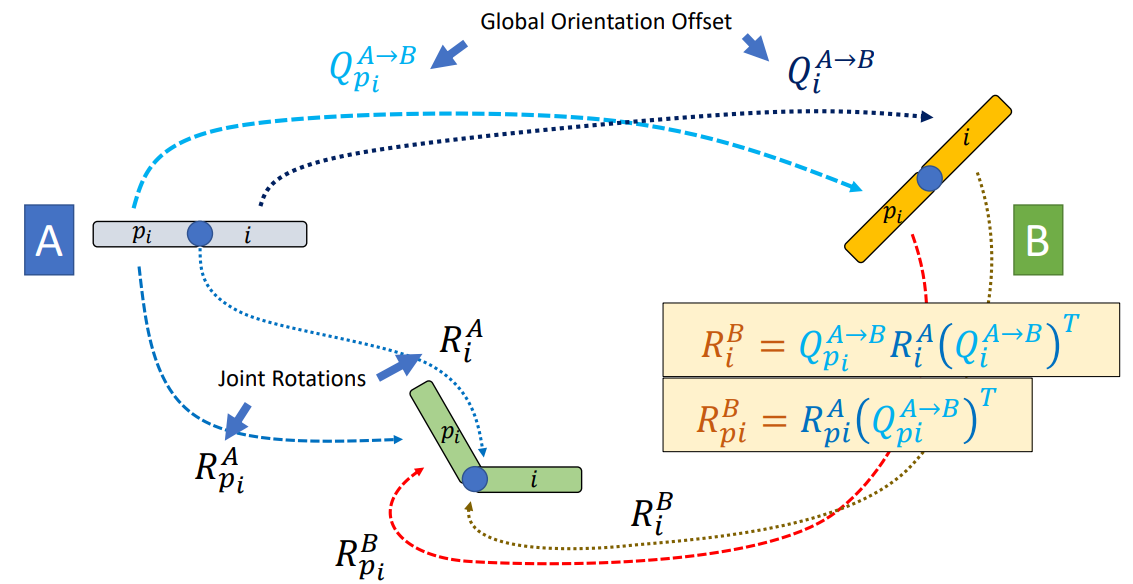
\includegraphics[totalheight=2in]{"./image/Retargeting.png"}
  \caption{Retargeting} \label{fig:Retargeting}
\end{figure}

记忆:$B$父旋转=父旋转*父朝向映射的逆, $B$子旋转=父朝向映射*子旋转*子朝向映射的逆。

最后是参考姿势到参考姿势的重定向,递归考虑。

实际情况,动捕的时候是人,角色却很复杂,比如人体脊柱一般2-3个关节,而角色可能有
7-8个关节,另外还有衣服,斗篷,道具等。大概列举如下:
\begin{itemize}
  \setlength{\itemindent}{2em}
  \item 不同数量的骨骼
  \item 骨骼名称不同
  \item 参考姿势不同
  \item 骨骼的大小不同
  \item 骨骼的拓扑结构不同
  \item ......
\end{itemize}

一个可能的重定向pipeline:
\begin{itemize}
  \setlength{\itemindent}{2em} 
  \item[1] 骨骼映射
  \item[2] 调整动捕数据大小,通常将根关节的位移缩放到虚拟角色和目标角色的腿长一致,至少能保证走路时,脚不会飘着
  \item[3] 处理关节T-pose的区别
  \item[4] 穿模修正,浮空,脚打滑等的IK后处理。
  \item[5] \dots 
\end{itemize}

\section{关键帧动画}
主要是插值。

\subsection{插值}
平滑度:Discontinuity, $C^{0}\text{-continuity}$,$C^{1}\text{-continuity}$,$C^{2}\text{-continuity}$。
位置,速度,加速度是否一致。或者连续,导数相等,二阶导数相等。$C^2$一般在物体建模中才会体现出效果来。

点集$D={(x_i, y_i)|i=0, \cdots, N }$的多项式$f(x)=a_0 + a_1 x + a_2 x^2 + 
\cdots + a_n x^n$拟合,其中$n=N-1$。容易得到
\begin{equation}
  \left[\begin{array}{c}
  a_0 \\
  a_1 \\
  \vdots \\
  a_n
  \end{array}\right]=\left[\begin{array}{ccccc}
  1 & x_0 & x_0^2 & \cdots & x_0^n \\
  1 & x_1 & x_1^2 & \cdots & x_1^n \\
  \vdots & \vdots & \vdots & \ddots & \vdots \\
  1 & x_N & x_N^2 & \cdots & x_N^n
  \end{array}\right]^{-1}\left[\begin{array}{c}
  y_0 \\
  y_1 \\
  \vdots \\
  y_N
  \end{array}\right]
\end{equation}
但,高阶多项式函数拟合容易\href{https://personal.math.ubc.ca/~peirce/M406_Lecture_3_Runge_Phenomenon_Piecewise_Polynomial_Interpolation.pdf}{龙格库塔现象}(误差受高阶项影响很大,不稳定,可至无穷大)。

解决办法,分段插值。 若线性,则$f(x)=S_i(x), x \in[x_i, x_{i+1}]$,
$S_i(x)=y_i + \frac{y_{i+1} - y_i}{x_{i+1}-x_i}(x-x_i)$。
若非线性,可选样条插值(可证明,固定两端点,中间人选2点固定,则四点组成的曲线,一定是三次多项式
$S_i = a_i x^3 + b_i x^2 + c_i x + d_i$)。
经典的有:三次样条,三次Hermite样条,Catmull-Rom样条。

对于三次样条,给定$N+1$个点,可分成$N$个片段,每个片段由一个样条逼近,则总共有$4N$个参数,因此需要至少$4N$个方程。
\begin{equation}
  \begin{aligned}
  \text { Interpolation condition: } & S_i\left(x_i\right)=y_i, \quad S_i\left(x_{i+1}\right)=y_{i+1} \\
  C^1 \text { continuity: } & S_{i-1}^{\prime}\left(x_i\right)=S_i^{\prime}\left(x_i\right) \\
  C^2 \text { continuity: } & S_{i-1}^{\prime \prime}\left(x_i\right)=S_i^{\prime \prime}\left(x_i\right) \\
  \text { boundary condition: } & S_0^{\prime}\left(x_0\right), S_{n-1}^{\prime}\left(x_n\right), S_0^{\prime \prime}\left(x_0\right), S_{n-1}^{\prime \prime}\left(x_n\right)
  \end{aligned}
\end{equation}
求解$4N \times 4N$可得。但此种方式求逆复杂,并且方程是整体关联的,牵一发而动全身。

希望插值函数有局部性,计算上没那么昂贵。三次Hermite样条给出了方案,只考虑当前段的首尾信息不考虑
前后的1,2此光滑性,这样就不受前后片段的影响,解决条件不够的方法,就是增加额外信息,
$S_i^{\prime}(x_i)=m_i, S_{i+1}^{\prime}(x_i)=m_{i+1}$,$m_i$表示$x_i$的速度。

把当前片段映射到$[0,1]$,用$t$表示,有:$S(t)=at^3 + bt^2 + ct + d$。将$m_i$(为了
方便,假设映射后的单位片段的左右速度为$m_i$)的值表示出来,有矩阵关系:
\begin{equation}
  \begin{aligned}
  S(t) & =a t^3+b t^2+c t+d \\
  & =\left[\begin{array}{llll}
  t^3 & t^2 & t^1 & 1
  \end{array}\right]\left[\begin{array}{cccc}
  2 & -2 & 1 & 1 \\
  -3 & 3 & -2 & -1 \\
  0 & 0 & 1 & 0 \\
  1 & 0 & 0 & 0
  \end{array}\right]\left[\begin{array}{l}
  y_i \\
  y_{i+1} \\
  m_i \\
  m_{i+1}
  \end{array}\right] \\
  & =\left[\begin{array}{c}
  2 t^3-3 t^2+1 \\
  -2 t^3+3 t^2 \\
  t^3-2 t^2+t \\
  t^3-t^2
  \end{array}\right]^T\left[\begin{array}{l}
  y_i \\
  y_{i+1} \\
  m_i \\
  m_{i+1}
  \end{array}\right]
  \end{aligned}
\end{equation}
左边每一行称为Hermite基函数,$H_i, i=0, 1, 2, 3$。更高维
$y, m$,对应了同样维度的$a, b, c, d$向量。

\subsection{插值和样条}
\begin{equation}
  \begin{aligned}
  S(t) & =a t^3+b t^2+c t+d \\
  & =\left[\begin{array}{c}
  2 t^3-3 t^2+1 \\
  -2 t^3+3 t^2 \\
  t^3-2 t^2+t \\
  t^3-t^2
  \end{array}\right]^T\left[\begin{array}{l}
  y_1 \\
  y_2 \\
  m_1 \\
  m_2
  \end{array}\right]
  \end{aligned}
\end{equation}

Catmull-Rom Spline是说:给定四点$P_0, P_1, P_2, P_3$,
有$y_1=p_1, y_2=p_2, m_1 = \frac{p_2 - p_0}{2(x_2 - x_0)},
m_2 = \frac{p_3 - p_1}{2(x_3 - x_1)}$。这里$1, 2$表示去上面第一个
片段$i=1$。

\subsection{旋转的插值}
\begin{figure}[htbp]
  \centering
  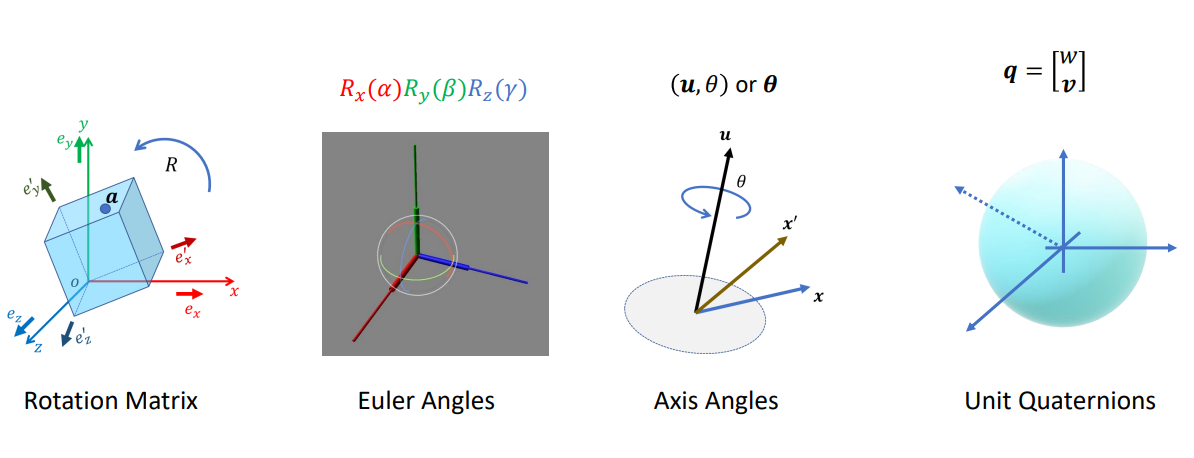
\includegraphics[totalheight=2in]{"./image/RotationRepresentations.png"}
  \caption{Rotation Representations} \label{fig:RotationRepresentations}
\end{figure}
SLERP for Quaternions \ref{WilliamRowanHamilton},本质上是一个线性插值。

如何实现四元数的非线性插值?\href{https://splines.readthedocs.io/en/latest/rotation/kochanek-bartels.html}{kochanek-bartels}。
该文讨论了四元数的贝塞尔曲线插值,效果比线性更平滑,但是在实现上,其加速度有时候抖动会比较大,
并且加速度的求解对应到曲面上的最小曲率问题,比较困难。
一般正确处理边界条件,效果差别不太大。

\section{数据驱动动画}
靠关键帧来生成动作,是一个劳动密集型工作。因为一般关键帧
的fps并不高,k帧挺麻烦。


动捕:使用动捕设备采集动作数据,或利用AI从视频中提取,或者生成。
使用动捕数据,可实现无人机的跟踪等各自应用。

惯性传感器,惯性测量单元(Inertial Measurement Unit, IMU)记六轴传感器,
包括3个加速度器和三个角速度器,记录关节点的相对运动,利用IK或优化的算法求解出每个
关节的旋转,得到运动数据。但是惯性传感器存在飘逸问题,传感器的飘逸,对加速度,速度的积分
得到传感器的位移,位移加上当前的位置得到全局的位置,而长时间的积分的误差导致位置存在偏差。
可以利用重力传感器,磁场传感器,光流传感器,来增加全局变量,来缓解飘逸问题。

基于光学的设备,反/发光标记点,若干相机组成的系统,来重建三维环境,从而得到位置信息。
比如:多视角几何通过几何相交等形状来确定点的位置。光学设备最大问题是场景问题,一般对场景
要求比较高。脸的动捕,会标记更多点,并且会戴额外的相机,对准脸。光学动捕需要处理丢失数据,
补点一般比较麻烦(按秒算钱,可以使用ML,AI来简化后处理流程)。

基于多视角相机来获取动捕数据,相机本身位置是固定的,可以省去标记点,但是准确度大大则扣。

RGBD相机,提供深度信息,从而可以重建三维物体。

单目相机的动作估计。信息不全,把三维姿态映射为二维,本身存在奇异性问题,
利用更多数据来缓解这个问题。

如何使用动捕数据?Motion Synthesis。 
CMU:数据比较老,比较多,质量比较插。\href{https://paperswithcode.com/dataset/lafan1}{lafan1}:数据较全,质量ok。

\begin{figure}[htbp]
  \centering
  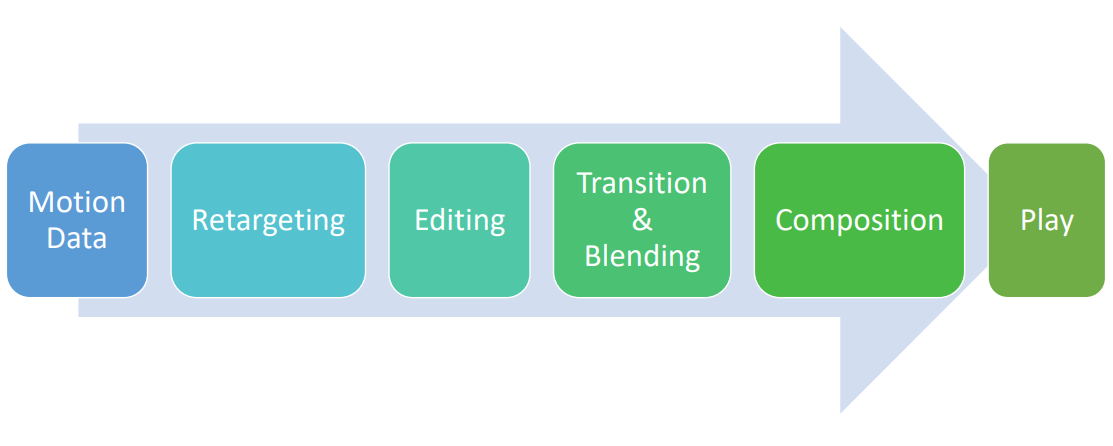
\includegraphics[totalheight=2in]{"./image/UsingMotionData.png"}
  \caption{Using Motion Data} \label{fig:UsingMotionData}
\end{figure}

动作连接,转移(Motion Transtion):将一段动作和另外一段动作衔接起来:
在第一个动作选择一帧,在第二个动作中找到类似的一帧,然后将两帧在时间上做一个对齐,该帧
称为切换帧,在各自切换帧前后分别选更多帧,做一个插值。$\boldsymbol{p}(t)=
(1-\phi(t))\boldsymbol{p}_0(i) + \phi(t)\boldsymbol{p}_1(i), 
\boldsymbol{p}=(t_0, R_0, R_1, \dots)$,$i$表示帧数。实际情况,不一定两边
都取若干帧,两者比例根据情况分析,最终达到足够平滑就行。但是这种方法,是不能处理
脚底打滑。比如,一段是向左走,一段是向右走。更好的处理方式,是先做对齐,下一段
动作和上一段目标动作做对齐。对齐什么,怎么对齐?对齐主要就是坐标系的选择,坐标系是跟着
物体一起移动,定义方式多种,这里介绍"Facing(Hidding, Moving) Frame"坐标系(朝向,原点位置),
原点跟随物体根关节一起移动,一般定义为根在地面的投影,局部坐标系的$z$轴一般定义为朝向,
实际定义方式多种,比如速度的方向,面向的方向(局部坐标系的$z$在世界坐标系的方向),
$z$轴,主要是假设角色坐标系是一个$y-up$坐标系,符合Unity,Maya等软件,
也符合渲染的设定。一般假设Facing Frame的旋转,是沿着$y$轴旋转,其次坐标原点只有平面$x-z$
的位移。$R=\theta \boldsymbol{e}_y, \boldsymbol{t}=(t_x, 0, t_y)$。

Facing Frame把朝向定义为根关节局部坐标的$z$轴,因此Facing Frame坐标系的朝向(旋转)是把
世界坐标的$z$轴转到局部坐标的$z$轴的矩阵。两个肩膀或两个髋关节的连线对应了局部坐标系
的$x$轴,因此其平均值可以看作当前坐标系的$x$轴,也可以定义,世界坐标系的$x$轴与两髋关节
的平均$x$方向的映射为朝向,另外一种思路,利用旋转的分解:$R=R_y R_{xz}$。
知道了根关节的朝向$R$后,希望可以分解出$R_y$。局部坐标轴的$y$轴到世界坐标的$y$轴,利用
叉乘,可以计算出两者的旋转矩阵$R^{\prime}$,有$R_y=R^{\prime}R$。因为$R^{\prime}$
使得局部的$y$与世界的$yt$重合,有了$R_y$,容易得到$R_{xz}=R^{T}_y R$。可以证明,$R_{xz}$
对应与在$x-z$平面上一向量的旋转。

有了如上定义,对于动作的每一帧,都可以计算其朝向坐标系$(R_0, t_0), (R_1, t_1)$。此时,将
两个动作连接,先对给定的两切换帧做对齐处理,然后插值。这里注意,某一段动画,确定好
切换帧的坐标系,其后帧均需按此坐标系表示。因此有
\begin{equation}
  \begin{aligned}
  R(i)&=R_0 R^{T}_1 R_1(i)\\
  \boldsymbol{t}(i)&=R_0 R_1 ^T (\boldsymbol{t}_1(i)-\boldsymbol{t}_1) + \boldsymbol{t}_0
  \end{aligned}
\end{equation}
$i$表示后续帧,$R(i),t(i)$分别表示后续帧的朝向和位置。

有时候根关节的运动是没有的,比如动捕数据去掉了根关节的运动信息,动画
师没有做根关节的运动。这种情况就只需要做姿态对齐。

Path Fitting:让角色跟着轨迹走。对于去除了跟关节运动的动画,
算出轨迹的方向(每一点的速度和位置),将其乘(?)到姿势上,就得到了沿着
轨迹的动画了。

动作合成:有很多动作,根据这些动作来生成新的动作。Motion Graphs动作图(02年)。
动作图的基本单元,动作片段。这就涉及到动作分割问题。主要思路是算动作
的距离图(距离的定义多样),用距离图的局部最小值作分割判断。


交互式动画Pipeline:
\begin{itemize}
  \setlength{\itemindent}{2em}
  \item 检查用户输入
  \item 检查环境
  \item 检查其他角色
  \item 确定是否迁移
  \item 获取下一个姿势
  \item 处理姿势
  \item 更新角色
  \item 更新环境
  \item \dots
\end{itemize}

Motion Matching每一帧的流程:
\begin{itemize}
  \setlength{\itemindent}{2em}
  \item 检查用户输入
  \item 根据输入,找到与当前状态最邻近的姿势
  \item 将两姿势做光滑连接
  \item next\_pose $=\min _{i \in \text { Dataset }}\left\|x_{\text {curr }}-x_i\right\|$
  \item $x:\text{特征向量}$ \begin{itemize}
    \item root linear/angular velocity
    \item position of end effectors w.r.t. root joint
    \item linear/angular velocity of end effectors w.r.t. root joint
    \item future heading position/orientation (e.g. in 0.5s, 1.0s, 1.5s, etc.)
    \item foot contacts
    \item ......
  \end{itemize}
  \item 光滑混合 \begin{itemize}
    \item \href{https://www.theorangeduck.com/page/spring-roll-call}{将当前姿势平滑地混合到目标姿势}
  \end{itemize} 
\end{itemize}

\section{基于学习的动画}
在常见人体的运动表示数据(姿态)组成的空间中,符合人体的运动一般是一个低维流形嵌入,否则
随机采样的动作,就是有效的。这也说明,人体运动数据的自由度,没有其表示数据的自由度
那么高。比如,一般走路时候,手是反向摆动,膝盖的不能向上旋转,人受物理定律限制,
一般是走在路面的。主成分分析是一个比较简单的寻找低维空间算法。

\subsection{主成分分析}
找维度之间的相关性,将点$\boldsymbol{x}_i$在$\boldsymbol{u}$作投影,使得
投影后的量最大限度的保持原有信息,分布范围比较大。

可用方差来刻画,求方向$\boldsymbol{u}$,已知点集$\boldsymbol{x}_i$在其上的
投影$\boldsymbol{u}:w_i=\boldsymbol{x_i}\boldsymbol{u}$,使得
$w_i$的方差$\frac{1}{N}\sum_{i}(w_i - \bar{w})^2$最大。
可以证明,令$X=\left[\begin{array}{c}
  \left(\boldsymbol{x}_0-\overline{\boldsymbol{x}}
  \right)^T \\ \left(\boldsymbol{x}_1-
  \overline{\boldsymbol{x}}\right)^T 
  \\ \cdots \\ \left(\boldsymbol{x}_N-\overline{\boldsymbol{x}}
  \right)^T\end{array}\right]$
则$\boldsymbol{u}$是$X^T X$的最大特征值对应的向量。

给定数据${\boldsymbol{x_i}}, \boldsymbol{x_i}\in \mathbb{R}^N$,PCA进一步
拓展了上面的步骤,给出了最佳的$k$个方向。有:

\begin{equation}
  \boldsymbol{x}_i=\overline{\boldsymbol{x}}+\sum_{k=1}^n w_{i, k} \boldsymbol{u}_{\boldsymbol{k}}
\end{equation}
其中$\boldsymbol{u}_k$称为第$k$个主成分。对应了第$k$大特征值的特征向量,
$w_{i, k}=(\boldsymbol{x_i} - \overline{x})\boldsymbol{u}_k$表示
$\boldsymbol{x_i} $在$\boldsymbol{u_i} $上的分数。

计算上,可以用协方差矩阵的特征分解来做。
\begin{equation}
  \Sigma=X^T X=U\left[\begin{array}{llll}
  \sigma_1^2 & & & \\
  & \sigma_2^2 & & \\
  & & \ddots & \\
  & & & \sigma_N^2
  \end{array}\right] U^T
\end{equation}
其中$\sigma_i \geq \sigma_j\geq 0\text{当}i<j, U = [\boldsymbol{u_1}, \dots, \boldsymbol{u_N}]$,
$U$正交。

应用例子:走路。走路由姿态构成,姿态由关节的旋转构成。比如$K\text{帧},N\text{个关节}$,则有数据
$A_{K \times N\times 3}$,则$X=(A-\bar{A})$。


角色在考虑先验动作下的IK模型。
\begin{equation}
  \label{IK4.8}
  \begin{aligned}
  F(\theta) & =\frac{1}{2} \sum_i\left\|f_i(\boldsymbol{\theta})-\widetilde{\boldsymbol{x}}_i\right\|_2^2 \\
  & +\frac{w}{2} \sum_k\left(\frac{(\boldsymbol{\theta}-\overline{\boldsymbol{\theta}}) \cdot \boldsymbol{u}_k}{\sigma_k}\right)^2 \\
  \boldsymbol{\theta} & =\left(\boldsymbol{t}_0, R_0, R_1, R_2, \ldots \ldots\right)
  \end{aligned}
\end{equation}
这里$i$表示多个关节。

理由如下:动作离分布越远,越不自然。因此对于一个姿态,其在主成分方向
上的投影值与方差值的比值和$\sum_{k}(\frac{w_{i,k}}{\sigma_k})^2$越
小越自然(动作越好)。比较\ref{IK3.11},3.11主要是限制关节的旋转角度幅度不能太大。

\subsection{数据分布}
假设动作服从一个概率分布,比如多峰高斯分布。以此可以从该分布中采样$\boldsymbol{x_i}\sim p(\boldsymbol{x})$。

高斯分布的最大似然估计建模方式,当协方差为对角阵时,该思路和主成分析等价。
\begin{equation}
  p(\boldsymbol{x})=\mathcal{N}\left(\mu_i, \Sigma_i\right)=\frac{1}{\sqrt{(2 \pi)^k|\Sigma|}} e^{-\frac{1}{2}(\boldsymbol{x}-\overline{\boldsymbol{x}})^T \Sigma^{-1}(\boldsymbol{x}-\overline{\boldsymbol{x}})}
\end{equation}
其中$\Sigma = \frac{1}{N}X^T X,X \text{定义如公式4.7}$。
对方差矩阵做特征值分解,若方差是对角阵,说明每一个分量相互独立,因此可将公式4.8写为
乘积的形式
\begin{equation}
  \label{IK4.10}
  \begin{aligned}
  p(\boldsymbol{x}) & =\prod_k \frac{1}{\sigma_k \sqrt{2 \pi}} e^{-\frac{1}{2}\left(\frac{w_k}{\sigma_k}\right)^2} \\
  w_k & =(\boldsymbol{x}-\overline{\boldsymbol{x}}) \cdot \boldsymbol{u}_k
  \end{aligned}
\end{equation}
其对数似然后和\ref{IK4.8}等价。推而广之,可将式\ref{IK4.8},\ref{IK4.10}推广为:
\begin{equation}
  F(\theta) =\frac{1}{2} \sum_i\left\|f_i(\boldsymbol{\theta})-
  \widetilde{\boldsymbol{x}}_i\right\|_2^2 
   -w\log p(\boldsymbol{\theta}) 
\end{equation}
或者进一步将第一部分抽象为和动作相关的特征信息(姿态序列,IK,关键帧,用户控制,环境限制),
第二部分抽象为和动作相关的先验信息。
\begin{equation}
  F(\boldsymbol{x}) =f(\boldsymbol{x})-w\log p(\boldsymbol{\theta}) 
\end{equation}

由PCA和高斯分布来建模先验分布的局限性比较大,一般只在较为简单的场景中有用。

\subsection{运动神经网络模型}
比较复杂的分布可以用神经网络来学习,同时可控性就降低了很多。

老人走路,高兴走路等,一整套运动序列可以用条件概率模型($X={x_1, \dots, x_T}, p(X|z), X=f(z)$)来建模控制过程。
后面的姿态是基于之前的姿态控制的。每一个姿态是前面姿势走过后,下一个姿势也是一个合理的姿势。因此可以用联合分布
来建模。$p(X|z)=p(x_1, \dots, x_T|z)=p(x_1)\Pi_{t}p(x_t|x_{t-1},\dots, x_1;z)$。
\begin{equation}
  \begin{aligned}
  p\left(x_1, x_2\right) & =p\left(x_2 \mid x_1\right) p\left(x_1\right) \\
  p\left(x_1, x_2, x_3\right) & =p\left(x_2, x_3 \mid x_1\right) p\left(x_1\right) \\
  & =p\left(x_3 \mid x_2, x_1\right) p\left(x_2 \mid x_1\right) p\left(x_1\right)
  \end{aligned}
\end{equation}
除了第一帧外,后面每一帧都由前面若干帧决定。$x_t=f(x_{t-1}, x_{t-2}, \dots, x_1; z)$
给定前面若干帧和隐变量,来预测当前帧。进一步简化,马尔可夫性:$x_t = f(x_{t-1};z)$。
此时概率密度函数为$p(X|z)=p(x_1, \dots, x_T|z)=p(x_1)\Pi_{t}p(x_t|x_{t-1};z)$。
如此,可逐步生成所有动作。前者在给定文字或语言情况下,根据内容生成动作比较符合,后者在
遥感控制,比如游戏中,更加适合。不过后者没有考虑未来信息,而前者因考虑了整体信息,所以包含
了一定的未来信息。

自回归模型:用过去的信息来预测下一时刻的状态,$x_t = f(x_{t-1})$。关键帧动画的插值也是类似的
思路。更广泛的用神经网络来表达学这种运动生成过程如下图:

\begin{figure}[htbp]
  \centering
  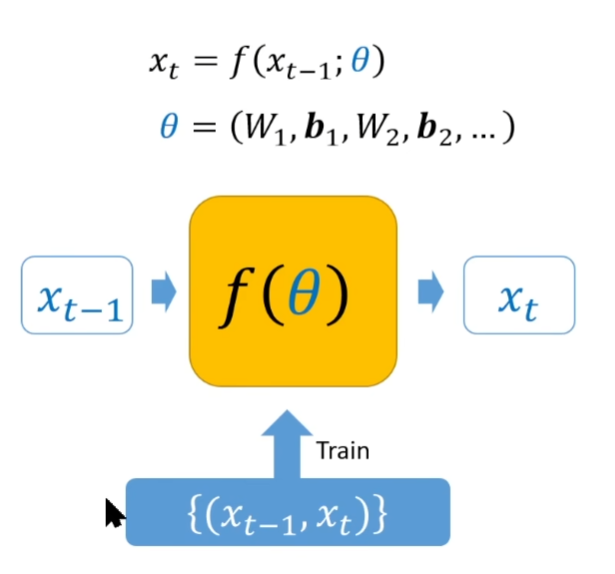
\includegraphics[totalheight=2in]{"./image/LearningMotionModel.png"}
  \caption{Learning Motion Model} 
  \label{fig:LearningMotionModel}
\end{figure}
其中$f(\theta)$是具有如下形式的前向神经网络:
\begin{equation}
  F(\boldsymbol{\theta})=f(\boldsymbol{x, \theta})=\sigma\left(\dots, \sigma\left(\boldsymbol{b}_3+W_3 \sigma\left(\boldsymbol{b}_2+W_2 
  \sigma\left(\boldsymbol{b}_1+W_1 \boldsymbol{x}\right)\right)\right)\right)
\end{equation}
神经网络一般使用随机梯度下降法优化。
\begin{equation}
  \begin{aligned}
    &\text{For a batch of random sample}:\left\{\left(x_{t-1}^{(i)}, x_t^{(i)}\right)\right\} \sim
   \left\{\left(x_{t-1}, x_t\right)\right\} \\
   & \text{Compute the approximate gradient}: \nabla_\theta F(\theta) \approx \sum_i \nabla_\theta\left(\left\|f\left(x_{t-1}^{(i)} ; \theta\right)-x_t^{(i)}\right\|\right)\\
  & \text{update}: \theta=\left(W_1, \boldsymbol{b}_1, W_2, \boldsymbol{b}_2, \ldots\right) \text{as}:
  \theta \leftarrow \theta-\alpha \nabla_\theta F(\theta)
  \end{aligned}
\end{equation}

歧义问题:数据集中,一时刻的动作,朝各个方向均有,也即$x_tf(x_{t-1})$
不是一个单射函数,这会给训练带来歧义问题,最终效果会转向某一时刻所有动作的
平均动作效果,可以增加额外的限制使其变为单射。即$x_t=f(x_{t-1};z)$。这里的
$z$被称为隐变量。如何找到合适的$z$可以参考相位函数神经网络。

\subsection{混合专家模型}
\begin{itemize}
  \item 思路一:多个神经网络模型的加权平均,$y=\sum_{i}w_i \theta_i$。
  \item 思路二:权重混合,$y=f(x;w_i \theta_i)$。
\end{itemize}

PFNN使用了权重混合专家模型思路。

\subsection{相位函数神经网络}
PFNN:PhaseFunctioned Neural Networks,论文作者\href{https://theorangeduck.com/page/projects}{blog},
论文的中文解读可参考\href{https://blog.csdn.net/zb1165048017/article/details/103990505}{PFNN中文解读}。
该文章证明了DL在优化运动控制问题上是可行的。论文作者的后续文章,Motion Matching有更多的使用价值。围绕该文思路,
优化主要围绕相位函数来做文章。网络结构并不复杂,重点在建模的思路。

缺点:细节无法复现,急转弯没有减速,调头。

后续工作Gating Network(对专家混合参数的优化):
\begin{itemize}
  \setlength{\itemindent}{2em}
  \item Mode-Adaptive Neural Networks for Quadruped Motion Control(18)
  \begin{itemize}
    \item 考虑了脚的速度
  \end{itemize}
  \item Local Motion Phases for Learning Mutil-Contact Character Movements(20)
  \begin{itemize}
    \item 考虑了手的速度
  \end{itemize}
  \item DeepPhase:Peridic Autoencoders for Learning Motion Phase Manifolds(22)
  \begin{itemize}
    \item 不用对每个部位定义相位函数,用傅里叶变换去学习相位函数的组合(复合相位函数)
  \end{itemize}
\end{itemize}

\subsection{生成模型}
对概率密度函数的直接建模,去显式的学习一个$p(X|z)$,而不是如上面
间接的学习中间的转移函数。
\begin{figure}[htbp]
  \centering
  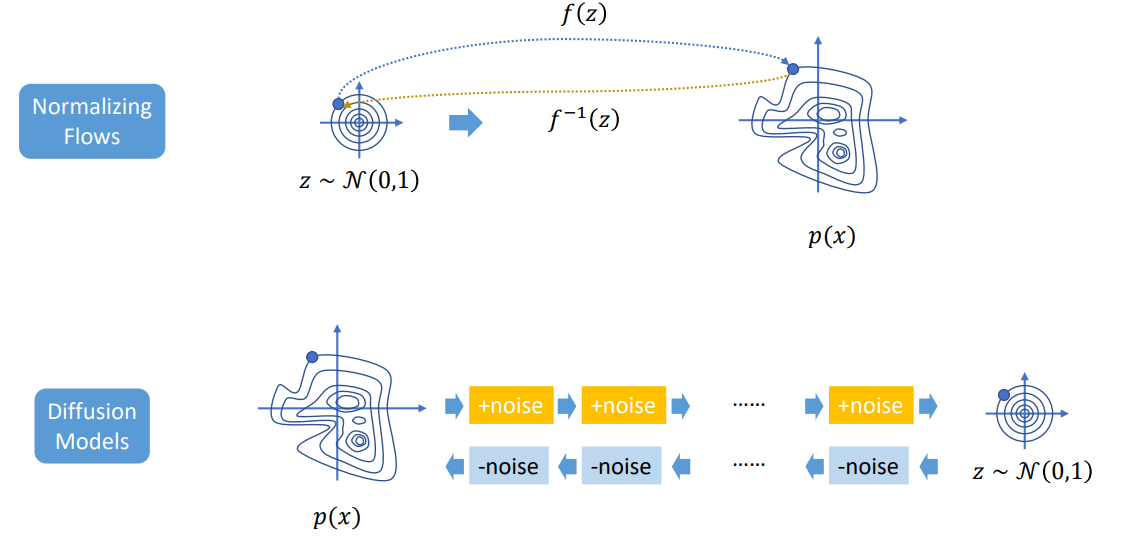
\includegraphics[totalheight=2in]{"./image/GenerativeModels.png"}
  \caption{Generative Models} \label{fig:GenerativeModels}
\end{figure}

列举几个参考文章。61分。

\newpage
\section{蒙皮和脸部动画}
骨骼发生形变(位移和旋转,$\boldsymbol{t}, R$)的同时,计算出其关联的顶点的
位移$\boldsymbol{x^{\prime}} \leftarrow \boldsymbol{x}$。具体来说就是朝向
和位移在$Q^{\prime} = RQ, \boldsymbol{o^{\prime}} =
\boldsymbol{o} + \boldsymbol{t} $变换下,$x$在变换后的骨骼下的世界坐标是什么。
首先将$x$转化到在原始骨骼下的局部坐标,$Q^{T}(x-o)$,然后可以得到在新的朝向,原点为
$Q^{\prime}, o^{\prime}$下的世界坐标$x^{\prime}=Q^{\prime}Q^{T}(x-o) + o^{\prime}$。
将$o$到$x$的向量记为$r$,则有:$r=Q^{T}(x-o), x^{\prime} = Q^{\prime}r + o^{\prime}$。
本质上就是一个从局部坐标系到全局坐标系的一个转换。

Bind/rest Pose:给出模型上每一个点在每个骨骼下的局部坐标表示。
模型一般创建为A-pose,而骨骼一般创建为T-pose或A-pose。
为了将两者联系起来,需要将骨骼变换到需要蒙皮的模型的初始姿势(A-pose)。
在这个姿势下,再去计算蒙皮上的每一个点相对于骨骼关节的距离,位置。这些局部
信息在计算蒙皮绑定的时候用到,比如上面的$r$。

考虑有两个骨骼的手臂,肩关节和肘关节。如图4.6,
\begin{figure}[htbp]
  \centering
  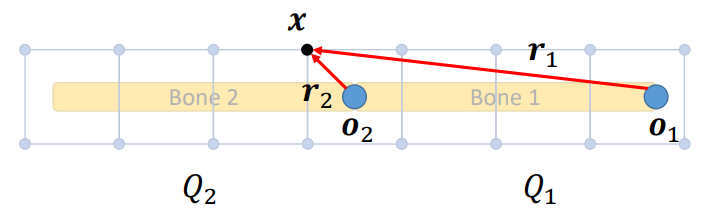
\includegraphics[totalheight=2in]{"./image/SkiningDeformation.png"}
  \caption{Skining Deformation} \label{fig:SkiningDeformation}
\end{figure}
有局部表示$\boldsymbol{r}_2=Q_2^T\left(\boldsymbol{x}-\boldsymbol{o}_2\right) \quad 
\boldsymbol{r}_1=Q_1^T\left(\boldsymbol{x}-\boldsymbol{o}_1\right)$。
对骨骼1,2分别做旋转$R_1, R_2$后朝向为$Q^{\prime}_1, Q^{\prime}_2$,
对于同一点$\boldsymbol{x}$,其世界坐标在两骨骼下有两种结果:
\begin{equation}
  \begin{aligned}
  & \boldsymbol{x}_1^{\prime}=Q_1^{\prime} \boldsymbol{r}_{\mathbf{1}}+\boldsymbol{o}_1^{\prime} \\
  & \boldsymbol{x}_2^{\prime}=Q_2^{\prime} \boldsymbol{r}_2+\boldsymbol{o}_2^{\prime}
  \end{aligned}
\end{equation}
为了消除歧义,一种方式是令两者的线性组合为最终结果:$x^{\prime}=w_1 x^{\prime}_1 + w_2 x^{\prime}_2$。

在角色中,一个点往往受到多个骨骼的同时控制,比如人体的腰部上某一点$x$,会受到脊柱上的关节,髋关节等的影响。
其局部表示为$r_j = Q_{j}^{T}(x - o_j)$,当对人体改变姿势后,其位置变为$x^{\prime} = \sum_{j}w_j(Q^{\prime}_j r_j + o^{\prime}_J)$。

\subsection{线性混合蒙皮}
Linear Blend Skinning:多个点变换后的世界坐标。
\begin{equation}
  \boldsymbol{x}_i^{\prime}=\sum_{j=1}^m w_{i j}\left(Q_j^{\prime} r_{i j}+\boldsymbol{o}_j^{\prime}\right)
\end{equation}
其中$w_{ij}$称为蒙皮权重。

简单变形为:
\begin{equation}
  \label{f:LBS}
  \begin{aligned}
  \boldsymbol{x}_i^{\prime} & =\sum_{j=1}^m w_{i j}\left(Q_j^{\prime} r_{i j}+\boldsymbol{o}_j^{\prime}\right) \\
  & =\sum_{j=1}^m w_{i j}\left(Q_j^{\prime} Q_j^T\left(\boldsymbol{x}_i-\boldsymbol{o}_j\right)+\boldsymbol{o}_j^{\prime}\right) \\
  & =\sum_{j=1}^m w_{i j}\left(Q_j^{\prime} Q_j^T \boldsymbol{x}_i+\left(o_j^{\prime}-Q_j^{\prime} Q_j^T o_j\right)\right) \\
  & =\sum_{j=1}^m w_{i j}\left(R_j \boldsymbol{x}_i+\boldsymbol{t}_j\right)
  \end{aligned}
\end{equation}
即,新的姿势下每个骨骼相对于Bind Pose下每个骨骼的相对旋转做加权平均再乘以Bind Pose下的位置,对应位移做加权平均。

在前面章节了解到,旋转矩阵是很难做线性插值的,得用四元数来做,因此这里旋转矩阵的线性组合,在实际中会出现被称为Candy-Wrapper Artifact的现象。
形象得可以理解为肘部旋转成麻花状。其优化思路,见四元数蒙皮小节。

但不管怎样,LBS在大多数场景下不会出现"麻花状",在工业中应用广泛,且对GPU比较友好。
\subsection{自动蒙皮}
有很多还可以研究,目前不是很成熟。
\begin{itemize}
  \item Learning Skeletal Articulations with Neural Blend Shapes
\end{itemize}

\subsection{双四元数蒙皮}
Dual Quaternion Skinning:在LBS中用四元数和SLERP插值。

这里不能简单的对\ref{f:LBS}做旋转的线性插值替换,原因是\ref{f:LBS}的旋转
公式$R_j x_i$是围绕$x_i$所在坐标系的原点旋转,也即插值中心不在$x_i$处,而在别处,
这样很多点按照插值替换操作,会出现比较大的位移变化效果。因此改进的基本出发点应该
需要把旋转和平移一起考虑,即射影变换,
$T_j=\left[\begin{array}{cc}R_j & \boldsymbol{t}_j \\ 0 & 1\end{array}\right] 
\in SE(3), R \in SO(3)$,简记为$T_j = [R_j | \boldsymbol{t_j}]$。

DQS的核心思想是将平移+旋转表达为一个对偶四元数,在对偶四元数中做intrinsic average插值。

\begin{definition}
  对偶数:$x = a + b\varepsilon$,其中$\varepsilon^2=0$。
\end{definition}
% \begin{definition}
%   共轭:对偶数$x$的共轭$\bar{x} = \overline{a+b\epsilon} = a - b\epsilon$。 
% \end{definition}
% \begin{definition}
%   乘积:两对偶数的乘积,$(a+b\epsilon)(c+d\epsilon)=ac +(ad+bc)\epsilon$
% \end{definition}
其共轭,乘积和复数对应定义思想一致。
\begin{definition}
  对偶四元数:$\widehat{\boldsymbol{q}}=\boldsymbol{q}_0+\varepsilon \boldsymbol{q}_{\varepsilon}$,其中
  $\varepsilon ^2 =0$。
\end{definition}
对偶四元数的共轭有三种定义:
$\begin{aligned} 
  & \mathrm{I}: \quad \widehat{\boldsymbol{q}}^*=\boldsymbol{q}_0^*+\varepsilon \boldsymbol{q}_{\varepsilon}^* \\ 
  & \text { II: } \quad \widehat{\boldsymbol{q}}^{\circ}=\boldsymbol{q}_0-\varepsilon \boldsymbol{q}_{\varepsilon} \\ 
  & \text { III: } \quad \widehat{\boldsymbol{q}}^{\star}=\boldsymbol{q}_0^*-\varepsilon \boldsymbol{q}_{\varepsilon}^* 
\end{aligned}$
但不管哪种,其都满足最后一点乘积的共轭等于顺序互换的共轭的乘积,且范数结果不变,
$\left(\widehat{\boldsymbol{q}}^*\right)^{\circ}=\left(\widehat{\boldsymbol{q}}^{\circ}\right)^* 
=\left(\widehat{\boldsymbol{q}}_1 \widehat{\boldsymbol{q}}_2\right)^{\times}=\widehat{\boldsymbol{q}}_2^{\times} \widehat{\boldsymbol{q}}_1^{\times} 
$ ,
范数$\|\widehat{\boldsymbol{q}}\|=\sqrt{\widehat{\boldsymbol{q}}^* \widehat{\boldsymbol{q}}}=\left\|\boldsymbol{q}_0\right\|+\frac{\varepsilon\left(\boldsymbol{q}_0 \cdot \boldsymbol{q}_{\varepsilon}\right)}{\left\|\boldsymbol{q}_0\right\|}$,
要使得$\widehat{\boldsymbol{q}}$为单位四元数,需要$\|\widehat{\boldsymbol{q_0}}\|,\boldsymbol{q_0} \boldsymbol{q_{\varepsilon}}=0$。

结合四元数的基本性质,有
\begin{proposition}
  \begin{enumerate}
    \item $s \widehat{\boldsymbol{q}}=s \boldsymbol{q}_r+s \boldsymbol{q}_{\varepsilon} \varepsilon$
    \item $\widehat{\boldsymbol{q}}_1+\widehat{\boldsymbol{q}}_2=\boldsymbol{q}_{r 1}+\boldsymbol{q}_{r 2}+\varepsilon\left(\boldsymbol{q}_{\varepsilon 1}+\boldsymbol{q}_{\varepsilon 2}\right)$
    \item $\widehat{\boldsymbol{q}}_1 \widehat{\boldsymbol{q}}_2=\boldsymbol{q}_{r 1} \boldsymbol{q}_{r 2}+\varepsilon\left(\boldsymbol{q}_{r 1} \boldsymbol{q}_{\varepsilon 2}+\boldsymbol{q}_{r 2} \boldsymbol{q}_{\varepsilon 1}\right)$
  \end{enumerate}
\end{proposition}

\begin{theorem}
  任何刚性变换$T\in SE(3)$能被转换为一个单位四元数表示。即
$
T=[R \mid \boldsymbol{t}] \rightarrow \widehat{\boldsymbol{q}}=\boldsymbol{q}_0+\varepsilon \boldsymbol{q}_{\varepsilon}
$,
其中
$\boldsymbol{q}_0=\boldsymbol{r}$,是$R$对应的四元数表示,
$\boldsymbol{q}_{\varepsilon}=\frac{1}{2} \boldsymbol{t r}$ 表示一个纯四元数,$\boldsymbol{t}=(0, t)$。
\end{theorem}

将一个向量$\boldsymbol{v}$用单位对偶四元数旋转,可表达为
\begin{equation}
  \widehat{\boldsymbol{v}}^{\prime}=\widehat{\boldsymbol{q}} \widehat{\boldsymbol{v}} \widehat{\boldsymbol{q}}^{\star},  
\end{equation}
其中向量$\boldsymbol{v}$需转化为对偶四元数形式
$ \hat{\boldsymbol{v}} =1+\varepsilon(0, v) =(1,0,0,0)+\varepsilon\left(0, v_x, v_y, v_z\right)$,
共轭为第\text{III}种定义方式。

对于四元数,我们有任何旋转能表示为两个四元数的形式,他们互为相反数,
同样,对于任何刚性变换$T\in SE(3)$也有类似的结论,互为相反数的对偶四元数
表示同样等价。

在大圆上有双重覆盖(Double Cover)的情况下,考虑到两点是最近点,表示的是同样的刚性变换,
又因为点的负数表示同样的旋转,因此可以将其中一点以圆心为对称点,对称到对面,使得两点
在同一个半圆内。也即任何两个变换,在圆周上的距离,都可以做到同一半圆内,
这种情况下,任何两点的插值,都可以做一个线性插值,然后单位化,投影到圆上。
\begin{equation}
  \begin{gathered}
  \widehat{\boldsymbol{q}}_t=(1-t) \widehat{\boldsymbol{q}}_{\mathbf{0}}+t \widehat{\boldsymbol{q}}_{\mathbf{1}} \\
  \Downarrow \\
  \widehat{\boldsymbol{q}}_t=\frac{(1-t) \widehat{\boldsymbol{q}}_0+t \widehat{\boldsymbol{q}}_{\mathbf{1}}}{\left\|(1-t) \widehat{\boldsymbol{q}}_{\mathbf{0}}+t \widehat{\boldsymbol{q}}_{\mathbf{1}}\right\|}
  \end{gathered}
\end{equation}
这就是DQS,不过同样存在角速度不恒定问题。对于四元数来说,SLERP能保持速度恒定,对对偶四元数,同样存在
类似的方法,这里略。

对偶四元数对LBS在Twist处,绕自传轴转180度的情况,效果是比较好的。
但它同样存在自己的问题,比如弯曲胳膊肘,胳膊肘部分会凸出,当Blend 权重
过渡比较光滑时,这种现象更明显。

\subsubsection{径向基函数插值}
Scattered Data Interpolation的一些解法:
\begin{enumerate}
  \setlength{\itemindent}{2em}
  \item 最小二乘
  \item 样条插值
  \item Inverse distance weighting
  \item 高斯过程
  \item RBF
  \item \dots
\end{enumerate}

Radial Basis Function (RBF) Interpolation:用来解决高维离散点插值问题的一种方法。

具体含义:空间中有一系列选定点,假设点以圆周的方式向外扩散,其他点由选定点来决定,决定
方式是点到选定点的距离为权重函数。

\begin{equation}
  y=\sum_{i=1}^K w_i \varphi\left(\left\|\boldsymbol{x} -\boldsymbol{x}_i\right\|\right)
\end{equation}
在给定的距离函数$\varphi$基础上,如何计算$w_i$?已知$f(x_i)=y_i$的情况下,由多项式插值待定系数法,
可写出:
\begin{equation}
  \begin{gathered}
  {\left[\begin{array}{cccc}
  R_{1,1} & R_{1,2} & \cdots & R_{1, K} \\
  R_{2,1} & R_{2,2} & & \vdots \\
  \vdots & & \ddots & \vdots \\
  R_{K, 1} & \cdots & \cdots & R_{K, K}
  \end{array}\right]\left[\begin{array}{c}
  w_1 \\
  w_2 \\
  \vdots \\
  w_K
  \end{array}\right]=\left[\begin{array}{c}
  y_1 \\
  y_2 \\
  \vdots \\
  y_K
  \end{array}\right]} \\
  R_{i, j}=\varphi\left(\left\|\boldsymbol{x}_i-\boldsymbol{x}_j\right\|\right)
  \end{gathered}
\end{equation}
解线性方程即可。

这里的距离函数一般有如下选择,不同距离在不同数据上存在不同的光滑性。
\begin{enumerate}
  \setlength{\itemindent}{2em}
  \item Gaussian: $\varphi(r)=e^{-(r / c)^2}$
  \item Inverse multiquadric: $\varphi(r)=\frac{1}{\sqrt{r^2+c^2}}$
  \item Thin plate spline: $\varphi(r)=r^2 \log r$
  \item Polyharmonic splines: $\varphi(r)=\left\{\begin{array}{l}r^k, \quad k=2 n+1 \\ r^k \log r, k=2 n\end{array}\right.$ 
\end{enumerate}

RBF可以用到对LBS的优化上,Pose Space Deformation,这里略。


\subsection{SMPL模型}
如何建模不同大小,不同体型的人体模型?

给定不同大小,不同身材的人体模型,利用PCA分析出不同特征的特征向量,
可以得到模型表示:$T(\beta)=\bar{T}+\sum_{m=1}^{|\beta|} \beta_m S_n$,其中
$\bar{T}$表示平均人,$S_n$表示形状基向量(体型)。同时考虑增加不同姿态的人体模型,
优化出姿态的形变部分,于是模型可以表达为:
\begin{equation}
  T(\beta, \theta)=\bar{T}+\sum_{m=1}^{|\beta|} \beta_m S_n+\sum_{n=1}^{|\theta|} \theta_n p_n
\end{equation}
这里的$P_n$表示对形变的修正,因为在不同姿势下,同样的人体在不同部分存在不同程度的变形。

因此在某一身体形状(身材)下,增加姿势混合形状,产生对应的形变效果,最后加上
蒙皮部分$x=SKIN(T(\beta, \theta), \theta, W)$,就形成了SMPL人体模型。 

\subsection{Blendshapes}
\href{http://www.cs.unc.edu/~jdh/documents/thesis_master.pdf}{基于变形迁移的表情克隆}。

\subsubsection{脸部动画}
脸部动画还有以骨骼驱动的形式,这里只简单说说BS方式。

脸部动画化 $=$ 平均脸 $+$ 一群人脸(PCA) $+$  表情模型(BS)。
$$
X=X_0+\sum_i \beta_i B_i^{\mathrm{ID}}+\sum_j \theta_j B_j^{\operatorname{Exp}}
$$

物理建模:略。

让脸动起来形成动画,有Riging,或脸部追踪(Face Tracking)或语音等方式。
脸部追踪:采集人脸的动作,将动作映射到虚拟角色上。检查人脸的特征点位置,
通过求解以BS为参数的IK问题。其优化目标可以为:
\begin{equation}
  \min _{\beta_i, \theta_j}\left\|X_0+\sum_i \beta_i B_i^{\mathrm{ID}}+\sum_j \theta_j B_j^{\operatorname{Exp}}-\quad Y \quad\right\|+E\left(\beta_i, \theta_j\right)
\end{equation}

语音驱动:把语言映射到BS参数或者骨骼驱动参数。可参考Omniverse(audio2mouth),具体略。

\begin{problemset}
  \item 实现重定向
  \item 实现LBS
  \item 实现DQS
  \item 生成动作,动捕数据帧数比播放帧数少,如何正确的播放?(插值,重新采样。)
\end{problemset}

\chapter{物理模拟和铰链刚体}
基于运动学的方式可以直接去会改变角色每个关节的角度,位置。基于运动学的方法很难
生成和环境交互比较强烈的动作,很多时候,环境的参数会影响动作的形式,同时也会存在非预期
的一些动作,这些情况,基于运动学的方式,是很难生成比较合理的动作。比如动捕中,角色
遭受击打后做的反应, 基于运动学的会预定义好这些动作,但在开放环境,比如VR场景里,
我们无法去估计用户的交互,这种基于运动学的方式就做不到合理的反馈。

基于物理的角色动画,九几年就有相关工作,但直到最近DeepMicMic的工作开始到ControlVAE,ASE等,
才逐渐的把基于物理的角色动画,越来越有希望的真正的用在实际工作中,去代替基于运动学的方法,
来实现一些比较好的效果。

基于运动学的方法是直接去设计角色的姿态,但在这个过程中,环境有变换,用户有交互,这些情况
都是基于运动数据来工作的,而基于物理仿真的角色动画思路则不同,它在模拟环境,当环境变换,和用户
有交互时,模拟器会根据牛顿定律等物理规律的计算反馈出新的运动姿势。一部分是仿真(模拟)在真实世界中的
物理运动方式,二部分是控制。

\section{仿真}
单个粒子的动力学
\begin{equation}
  \begin{aligned}
  & a=f(x, v, t) / m \\
  & v=v_0+\int_{t_0}^t a d t \\
  & x=x_0+\int_{t_0}^t v d t
  \end{aligned}
\end{equation}
当$f$是个常数时是我们熟悉的一元二次函数,但大部分时候,$f$是和速度,位置(弹簧,胡克定律),时间
有关的,甚至没有一个显式的表达式。这种情况,预测粒子在未来某时刻的位置,就变得比较困难。

对于非线性,甚至非显示式子的函数的积分,往往需要离散化,设每片段为$h$,然后利用数值积分的方式,
来计算。对于单个粒子的情况,容易有:
\begin{equation}
  \begin{aligned}
  & v_{n+1}=v_n+a_n h \\
  & x_{n+1}=x_n+v_n h
  \end{aligned}
\end{equation}
和
\begin{equation}
  \begin{aligned}
  & v_{n+1}=v_n+a_{n+1} h \\
  & x_{n+1}=x_n+v_{n+1} h
  \end{aligned}
\end{equation}
前者被称为Explicit/Forward 欧拉积分,后者称为Implicit/Backward欧拉积分。因为后者需要
未来的加速度信息,这个需要对整体求解方程,其计算量比较大,以及收敛速度比较缓慢。因此有
两者的结合,
\begin{equation}
  \begin{aligned}
  & v_{n+1}=v_n+a_{n} h \\
  & x_{n+1}=x_n+v_{n+1} h
  \end{aligned}
\end{equation}
被称为Symplectic/Semi\-implicit欧拉积分。

考虑一个以质心为坐标原点的弹簧系统,质量、进度系数、位置、速度分别为$m,k,x,v$,由胡克定律有$f=-kx$。
容易写出其Explicit,Semi\-implicit,Implicit欧拉积分方程:
\begin{equation}
  \begin{aligned}
  v_{n+1}=v_n-\frac{k x_n}{m} h &\quad v_{n+1}=v_n-\frac{k x_n}{m} h &
  v_{n+1}=v_n-\frac{k x_{n+1}}{m} h \\
  x_{n+1}=x_n+v_n h &\quad  x_{n+1}=x_n+v_{n+1} h &x_{n+1}=x_n+v_{n+1} h
  \end{aligned}
\end{equation}
其对应的矩阵表示分别为:
\begin{equation}
  \left[\begin{array}{l}
  v_{n+1} \\
  x_{n+1}
  \end{array}\right]=\left[\begin{array}{cc}
  1 & -\hat{k} h \\
  h & 1
  \end{array}\right]\left[\begin{array}{l}
  v_n \\
  x_n
  \end{array}\right] \quad\left[\begin{array}{l}
  v_{n+1} \\
  x_{n+1}
  \end{array}\right]=\left[\begin{array}{cc}
  1 & -\hat{k} h \\
  h & 1-\hat{k} h^2
  \end{array}\right]\left[\begin{array}{c}
  v_n \\
  x_n
  \end{array}\right] \quad\left[\begin{array}{cc}
  1 & \hat{k} h \\
  -h & 1
  \end{array}\right]\left[\begin{array}{l}
  v_{n+1} \\
  x_{n+1}
  \end{array}\right]=\left[\begin{array}{l}
  v_n \\
  x_n
  \end{array}\right]
\end{equation}其中$\hat{k}=k/m$。
关于该质点系统的三种积分方式,对应的收敛性,稳定性,有如图\ref{fig:EulerIntegration}所示规律。
\begin{figure}[htbp]
  \centering
  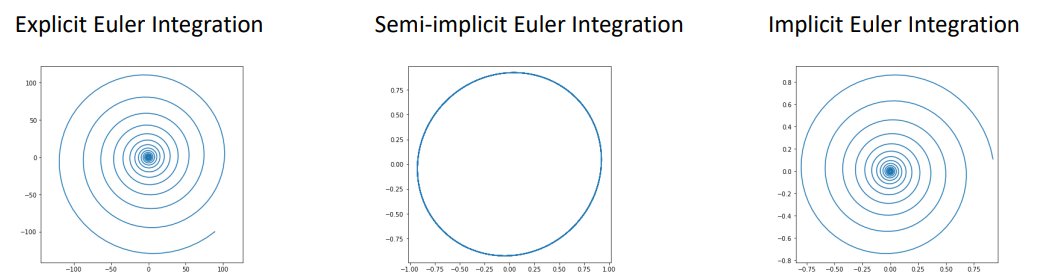
\includegraphics[width=0.6\textwidth]{./image/EulerIntegration}
  \caption{Euler Integration \label{fig:EulerIntegration}}
\end{figure}

更高级的积分方式:
\begin{enumerate}
  \setlength{\itemindent}{2em}
  \item Runge–Kutta methods
  \item  Variational integration
  \item Position-based dynamics (PBD),实际生产环境中主要使用,因其可实现并行
  \item ......
\end{enumerate}

\section{刚体动力学}
刚体是一种理想的假设,假设物体运动过程中不发生形变(实际物体受到相对论的限制,运动物体不可能不发生形变,否则速度可以达到无限大)。
对于刚体来说,其组成的粒子之间的局部坐标关系是不变的。
铰链刚体是由多个骨骼由关节点链接的刚体系统,每个骨骼均是一个刚体。

给定一个物体,选定某质点确定其位置为$x$,同时若给定刚体在世界坐标系中的朝向$R$,
则刚体中每个点的位置均可计算出来,不妨设点 $x^\prime$相对$x$的
位移设为$r_0$,则有$x^{\prime} = x + R r_0 = x + r$。

当物体在空间中运动时,可以计算每个质点的速度,加速度等基本信息。比如点$x^\prime$的速度
$v=\frac{d x^{\prime}}{d t} \Leftrightarrow \dot{x}^{\prime}=\dot{x}+\dot{R} r_0$。
这里旋转矩阵$R$关于时间的导数如何计算?由$RR^T = I$,可得$\dot{R}R^T + (\dot{R}R^T)^T=0$,
也即$\dot{R}R^T=\left[\begin{array}{ccc}
  0 & -\omega_z & \omega_y \\
  \omega_z & 0 & -\omega_x \\
  -\omega_y & \omega_x & 0
  \end{array}\right]=[\omega]_{\times}$
因此$\dot{R}=[\omega]_{\times}R$,其中$\omega$是角速度。
也即
\begin{equation}
  \label{dv:dt}
  v^{\prime}=v + \omega\times r
\end{equation}
利用Rodrigues'旋转公式可以证明:
\begin{equation}
  \begin{aligned}
  & \delta x= x^{\prime}-\boldsymbol{x} \\
  &=(\sin \theta) \boldsymbol{u} \times \boldsymbol{x}+(1-\cos \theta) \boldsymbol{u} \times(\boldsymbol{u} \times \boldsymbol{x}) \\
  & \Downarrow \\
  & \dot{\boldsymbol{x}}=\frac{d \boldsymbol{x}}{d t}= \frac{d \boldsymbol{x}}{d \theta} \cdot \frac{d \theta}{d t}=\dot{\theta} \boldsymbol{u} \times \boldsymbol{x} \\
  & \Downarrow \\
  &\dot{\boldsymbol{x}}=\boldsymbol{\omega} \times \boldsymbol{x}
  \end{aligned}
\end{equation}
因此对于给定物体$x, R$,以速度,角速度为$v, \omega$经过$\delta t$后,其点$x$变为$x^\prime$,朝向变为$R^\prime$,
有
\begin{equation}
  \begin{aligned}
  & x^{\prime}=x+\delta t \cdot v \\
  & R^{\prime}=R+\delta t \cdot[\omega]_{\times} R
  \end{aligned}
\end{equation}
用线性去逼近非线性的旋转,新的旋转矩阵需要被正交化,否则误差越来越大。而矩阵正交化可以使用
\href{https://en.wikipedia.org/wiki/Gram%E2%80%93Schmidt_process}{格拉姆-施密特正交化}方法,
可是格拉姆-施密特正交化法计算量比较大,可以利用四元数的单位化来替换。
此时公式变为:
\begin{equation}
  \begin{aligned}
  & x^{\prime}=x+\delta t \cdot v \\
  & q^{\prime}=q+\delta t \cdot\dot{q}
  \end{aligned}
\end{equation}其中$q^{\prime}$需要被单位化。

现在问题变为四元数如何求导。答案是$\dot{q}=\frac{1}{2}\bar{\omega}q,\bar{\omega}=(0, \omega)$。

运动学:$x, R; v, \omega; a, \alpha; ...$,动力学:$p, L; F, \tau$,这里$L=mr\times v=r \times p$表示角动量,
$r$表示粒子(质点)$x$相对于参考点$o$的方向(角动量必须有一个参考点,比如质心)。
$\tau=r\times F$表示将$F$施加在$x$上产生的力矩。两者的区别,可以认为是考虑了质量$m$与否。

刚体:认为是大量质点组成的系统。对于$m_i, x_i, v_i$,有$M=\sum_i m_i, x_c=\frac{\sum_i m_i x_i}{\sum_i m_i},
v_c=\frac{\sum_i m_i v_i}{\sum_i m_i}$。动量$p=\sum_i m_i v_i$,相对参考点$o$的
角动量$L_o = \sum_i m_i r^{\prime}_i \times v_i$。当参考点选为质点$x_c$,时,
角动量为$L_{x_c}=\sum_i m_i r_i \times v_i$。
由公式\ref{dv:dt}可得角动量$L=\sum_i -m_i [r_i]_{\times}^2\omega$。因给个质点的
角速度$\omega$都相同,令$I=\sum_i -m_i [r_i]_{\times}^2$,有$L=I \omega$,$I$称为转动惯量(Moment of Inertia)。
转动惯量是一个$3\times 3$的矩阵,本质上是质量在角速度上的类比,也就是说转动惯量小的,会更加容易旋转。由角动量守恒定律,
转动惯量变大时,速度变小。同时,转动惯量在旋转不同的状态下,其转动惯量不同。具体来说有如下关系:
\begin{figure}[htbp]
  \centering
  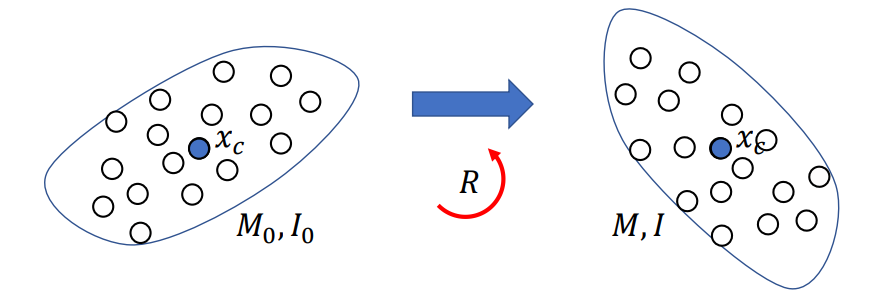
\includegraphics[width=0.6\textwidth]{./image/MomentofInertia.png}
  \caption{Moment of Inertia \label{fig:MomentofInertia}}
\end{figure}

\begin{equation}
  \begin{aligned}
  \text{利用:}
  & (R r) \times x=R\left(r \times\left(R^T x\right)\right) \\
  & {[R r]_{\times}=R[r]_{\times} R^T} \\
  & {[R r]_{\times}^2=R[r]_{\times}^2 R^T} \\
  \text{可得:}
  & M=M_0 \\
  & I=R I_0 R^T \\
  &
  \end{aligned}
\end{equation}
这里$I=RI_0 R^R$,有$I_0=diag(I_1, I_2, I_3)$。意思是说,可以找到一个旋转$R$,在这个旋转下,转动惯量$I$可以写为对角阵。
其中$I_i, i=1, 2, 3$称为转动惯量的主轴。

质心坐标系:是针对当前时刻,以质心为坐标系,不随时间而改变。可以理解为不同帧用各自的质心为原点的
坐标系,局部坐标系。

对刚体施加一个力,若力不在质心,会对物体在质心上产生两个效果,移动和旋转。
其旋转对应的力矩$\tau$等于$r \times f$,$r,f$分别表示作用点到质心的向量,
作用在作用点上的力大小。也存在,直接施加一个力矩。相当于,在刚体的两个点上,加了大小相等,
方向相反的力。或者多个点,多个力,但力的和为0。这些力对质心产生了转动惯量。
最终,我们可以理解为,对刚体的作用,等价于对质心的作用,一个力,一个转动惯量(所有力矩的求和)。
可表为$p=Mv_c, L=I\omega, f = \sum_i f_i, \tau=\sum_i \tau_i$。

运动学的量,方向$R$,位置$x$,速度$v$,角速度$\omega$。动力学的量,惯量$p$,角动量$L$,力$f$,力矩$\tau$。
质量$m$和转动惯量$I$。知道$m, I, p, L$能得到$v, \omega$。而$f, \tau$和两动量$p, L$之间是啥关系?
这个关系被称为运动学公式。

牛顿第二定律:
\begin{equation}
  f=Ma=\frac{d p}{d t}\Rightarrow M \dot{v}=f
\end{equation}
是一个运动学公式,它只关心物体的平动,不关心物体的旋转。

欧拉运动定律: 
\begin{equation}
  \tau = \frac{d L}{d t}\Rightarrow I \dot{\omega} + \omega\times I\omega =\tau
\end{equation}
说明了角动量的导数等于力矩,它考虑了物体的旋转。
\begin{proof}
  \begin{equation*}
    \begin{aligned}
      \dot{I}&= \frac{d}{d t}(RI_0 R^T)\\
      &=\dot{R}I_{0}R^T \\
      &=[\omega]_{\times}RI_0 R^{T}+RI_0 R^T \\
      & ------\Downarrow ------\\
     \dot{I}\omega & = \omega \times I\omega + I(-\omega \times \omega)
    \end{aligned}
  \end{equation*}
\end{proof}
牛顿-欧拉方程,被称为刚体运动方程。它告诉我们对于一个物体,知道外力和外力矩的情况下,可以计算
其加速度和角加速度,在给定初始速度和初始角速度的情况下,可以对其未来进行模拟。


\subsection{刚体运动方程}
回到上小节,将牛顿欧拉方程合在一起,有:
\begin{equation}
  \left[\begin{array}{cc}
  m I_3 & 0 \\
  0 & I
  \end{array}\right]\left[\begin{array}{c}
  \dot{v} \\
  \dot{\omega}
  \end{array}\right]+\left[\begin{array}{c}
  0 \\
  \omega \times I \omega
  \end{array}\right]=\left[\begin{array}{c}
  f \\
  \tau
  \end{array}\right]
\end{equation}

考虑其数值计算(刚体模拟):
\begin{equation}
  \label{bodysimulation:neumerail}
  \frac{1}{h}\left[\begin{array}{cc}
  m I_3 & 0 \\
  0 & I_n
  \end{array}\right]\left[\begin{array}{c}
  v_{n+1}-v_n \\
  \omega_{n+1}-\omega_n
  \end{array}\right]+\left[\begin{array}{c}
  0 \\
  \omega_n \times I_n \omega_n
  \end{array}\right]=\left[\begin{array}{l}
  f \\
  \tau
  \end{array}\right]
\end{equation}
其中$I_n$(当前时刻)可为$I_{n+1}$,但这样会使得方程的求解比较复杂,同样
$\omega_n \times I_n \omega_n$也如此。

具体讲$I_n = R_n I_0 R^{T}_n$,由当前刚体的朝向和初始转动惯量来构造\ref{bodysimulation:neumerail},
可计算出$v_{n+1}, \omega_{n+1}$,
然后由欧拉积分得到
\begin{equation}
  \begin{aligned}
  & x_{n+1}=x_n+h v_{n+1} \\
  & q_{n+1}=q_n+\frac{h}{2} \bar{\omega}_{n+1} q
  \end{aligned}
\end{equation}

上面只考察了一个刚体,对于两个刚体$m_i, I_i, x_i, R_i, v_i, \omega_i$有:
\begin{equation}
  \label{twobodynolink}
  \left[\begin{array}{llll}
  m_1 I_3 & & & \\
  & I_1 & & \\
  & & m_2 I_3 & \\
  & & & I_2
  \end{array}\right]\left[\begin{array}{c}
  \dot{v}_1 \\
  \dot{\omega}_1 \\
  \dot{v}_2 \\
  \dot{\omega}_2
  \end{array}\right]+\left[\begin{array}{c}
  0 \\
  \omega_1 \times I_1 \omega_1 \\
  0 \\
  \omega_2 \times I_2 \omega_2
  \end{array}\right]=\left[\begin{array}{c}
  f_1 \\
  \tau_1 \\
  f_2 \\
  \tau_2
  \end{array}\right]
\end{equation}
简写为:
\begin{equation}
  M \dot{v}+C(\boldsymbol{x}, \boldsymbol{v})=\boldsymbol{f}
\end{equation}

但这只是将两个刚体写在一起而已,并没有考虑两者的相互联系,对于角色来说,
两个刚体是需要铰链在一起的,否则对方程\ref{twobodynolink}做积分,两者会分开。
对于连在一起的刚体,可以认为两刚体有一个公共点(关节joint),彼此施加一个等大反向的
力,不妨记为$\boldsymbol{f_J}$,见\ref{fig:TwoLinksJoint}。
\begin{figure}[htbp]
  \centering
  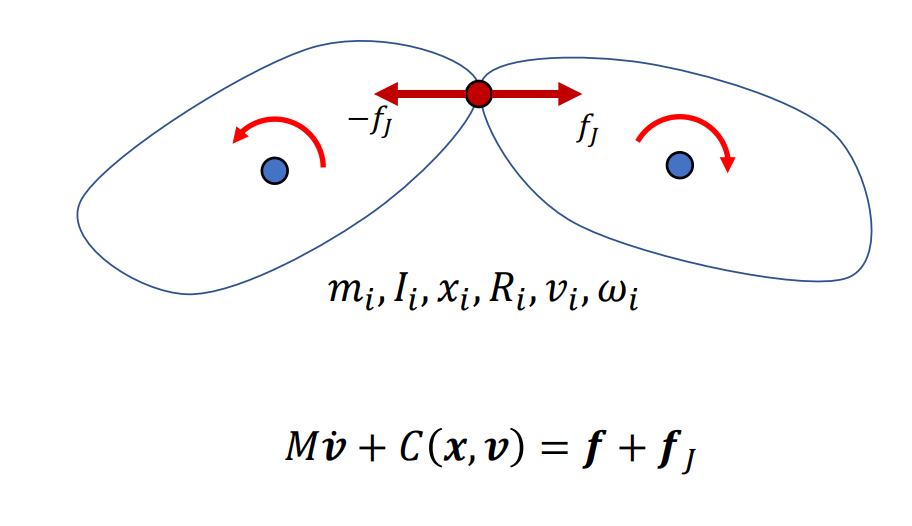
\includegraphics[totalheight=1in]{"./image/TwoLinksJoint.png"}
  \caption{Two Links and a Joint} \label{fig:TwoLinksJoint}
\end{figure}
于是两个铰链在一起的刚体的运动方程可简记为
$M \dot{v}+C(\boldsymbol{x}, \boldsymbol{v})=\boldsymbol{f} + \boldsymbol{f_J},$
这里$f$已知,$f_J$未知。

考虑一个刚体沿着给定的的曲线$g(x)=C$运动。两边对时间求导,$\frac{d}{d t}g(x)=0, 
\frac{\partial g}{\partial x}\cdot \frac{\partial x}{\partial t}=0$,
得到$Jv=0, J=[\nabla g ]^T$($g$的梯度的转置),这代表一个约束,即在任何时刻,物体沿着给定轨道
的速度满足上式子。因物体在轨道上运动,因此必然有外力作用,记为$f_c$,约束力不应该产生能量。
即约束力必然和物体的运动方向垂直。因$f_c \cdot v = 0 \Longleftrightarrow f^{T}_c v = 0$,
有$J v = 0 \Rightarrow f_c = J^{T}\lambda,\lambda \in \mathbb{R}$,说明施加的力和雅可比矩阵的转置共线。

得到带有限制的运动学方程:
\begin{equation}
  \begin{aligned}
  M \dot{v} & =f+J^T \lambda \\
  J v & =0
  \end{aligned}
\end{equation}
离散化形式为:
\begin{equation}
  \begin{gathered}
  M \frac{v_{n+1}-v_n}{h}=f+J^T \lambda \\
  J v_{n+1}=0
  \end{gathered}
\end{equation}
方程中已知$v_n$,$\lambda, v_{n+1}$未知,两方程联立求解$v_{n+1}, \lambda$。

上面的问题是假设当前时刻,满足$J v_{n+1}=0$,但实际我们是让物体沿着给定轨道运动,位置
是由速度一阶线性逼近的,因此在积分后,会存在误差。解决办法是让等式右边不等于0:
$J v_{n+1}=\alpha \frac{C - g(x_n)}{h}$。偏差乘以系数$\alpha$表示需要用多快的速度
将偏离物体拉回来,$\alpha$通常被称为ERP,error reduction parameter。此时求解方程,
形式等价于$JM^{-1}J^T \lambda=c_n$。等式左边的矩阵有可能奇异,解决办法仍然是加扰动,
$(JM^{-1}J^T  + \beta I )\lambda=c_n$,$\beta$:constaint force mixing(CFM)。

对于Joint Constraint,中间链接两个刚体点不会变为两个点,也即点相对于
两个刚体($m_i,I_i,R_i,v_i,\omega_i$)的中心位置($x_i$)的偏移向量($r_i$)在局部坐标系下是不变的。可表达为:
$x_1 + R_1 r_1 = x_J = x_2 + R_2 r_2$。两边对时间求导得到:
\begin{equation}
  \left[\begin{array}{llll}
  I_3 & -\left[r_1\right]_{\times} & -I_3 & {\left[r_2\right]_{\times}}
  \end{array}\right]\left[\begin{array}{l}
  v_1 \\
  w_1 \\
  v_2 \\
  w_2
  \end{array}\right]=0
  \end{equation}
简写为$J v=0$,为约束方程。

将两个刚体在一起的运动方程和两个刚体的约束方程,两者结合起来。构成两个带有关节约束的刚体系统
的运动方程和约束方程:
\begin{equation}
  \label{constrain::eqjoint}
  \begin{array}{r}
  {\left[\begin{array}{llll}
  m_1 I_3 & & & \\
  & I_1 & & \\
  & & m_2 I_3 & \\
  & & I_2
  \end{array}\right]\left[\begin{array}{l}
  \dot{v}_1 \\
  \dot{\omega}_1 \\
  \dot{v}_2 \\
  \dot{\omega}_2
  \end{array}\right]+\left[\begin{array}{c}
  0 \\
  \omega_1 \times I_1 \omega_1 \\
  0 \\
  \omega_2 \times I_2 \omega_2
  \end{array}\right]=\left[\begin{array}{c}
  f_1 \\
  \tau_1 \\
  f_2 \\
  \tau_2
  \end{array}\right]+\left[\begin{array}{c}
  I_3 \\
  {\left[r_1\right]_{\times}} \\
  -I_3 \\
  -\left[r_2\right]_{\times}
  \end{array}\right] \lambda} \\
  J v=0
  \end{array}
\end{equation}
求解得到约束力$\lambda$的大小,以及下一时刻每个刚体的速度,并且保证两个刚体在运动过程中不分开。

\begin{figure}[htbp]
  \centering
  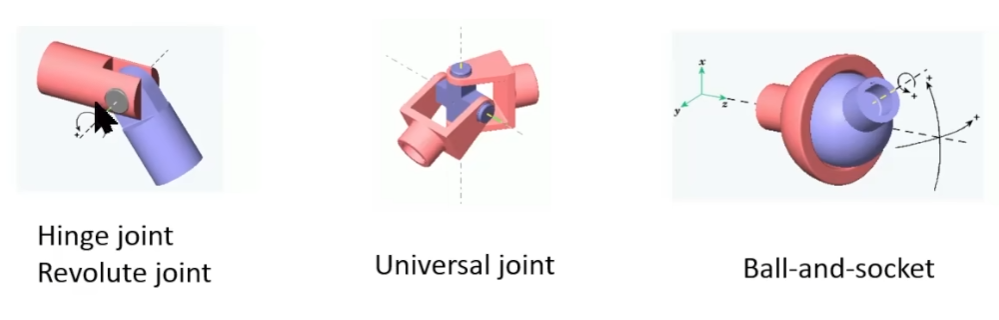
\includegraphics[totalheight=1in]{"./image/JointType.png"}
  \caption{Joint Type} \label{fig:JointType}
\end{figure}

这种约束本质上是Ball-and-socket的约束。但是对于Hinge/Revolute joint则需要更多关于角速度的约束,
Universal joint同理。总而言之,对不同类型的关节,对应了各自的约束形式。
对于Hinge/Revolute joint其约束形式如下:
\begin{equation}
  \left[\begin{array}{cccc}
  I_3 & -\left[r_1\right]_{\times} & -I_3 & {\left[r_2\right]_{\times}} \\
  ? & ? & ? & ?
  \end{array}\right]\left[\begin{array}{c}
  v_1 \\
  w_1 \\
  v_2 \\
  w_2
  \end{array}\right]=0
\end{equation}
增加了一行关于角速度的约束。

当多个关节点铰链在一起的时候,方程本质是不变的,只是方程的规模变大了。
\begin{equation}
  \begin{aligned}
  M \dot{\boldsymbol{v}}+C(\boldsymbol{x}, \boldsymbol{v}) & =\boldsymbol{f}+\boldsymbol{J}^T \boldsymbol{\lambda} \\
  J \boldsymbol{v} & =0
  \end{aligned}
\end{equation}

以上均没有考虑物体怎么站在地面上的问题,都只是在空中随意运动。考虑地面问题,需要考虑两点,
碰撞检测和接触建模。
\begin{figure}[htbp]
  \centering
  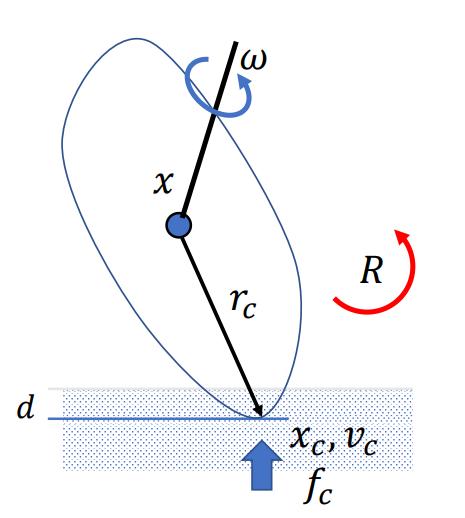
\includegraphics[totalheight=1.5in]{"./image/Contact.png"}
  \caption{Contact} \label{fig:Contact}
\end{figure}

假设已计算出碰撞点,一种思路是用线性模型来建模物体碰撞,比如弹簧模型。
\begin{equation}
  \begin{aligned}
  f_n & =-k_p d-k_d v_{c, \perp} \\
  f_t & =-\mu f_n \frac{v_{c, \|}}{\left\|v_{c, \|}\right\|}
  \end{aligned}
\end{equation}
在上式中,地面给物体的支持力,用一个弹簧模型来建模,其中深度$d>0$,第二部分是阻尼项,和速度相关。$f_t$表示
动摩擦带来的摩擦力,同时大小和速度相反,等于支持力乘以一个系数(静摩擦略)。
为了不让效果下陷很明显,一般$k_p$需要很大,才能保证陷入的深度比较小,但太大会导致
仿真的数值不稳定,为了让其稳定,需要设定更小的步长。

另外一种思路,把接触点建模成一个约束。主要关心这个点与接触面垂直的方向,在这个方向上,接触点的位置应该满足
什么条件。
在图\ref{fig:Contact}中,可以算出接触点在垂直方向上的速度$v_c$有如下关系:
\begin{equation}
  \begin{aligned}
  & x_c=x+r_c \\
  & v_c=v+\omega \times r_c=J_c\left[\begin{array}{l}
  v \\
  \omega
  \end{array}\right] \\
  & v_{c, \perp}=v+\omega \times r_c=J_{c, \perp}\left[\begin{array}{l}
  v \\
  \omega
  \end{array}\right]
  \end{aligned}
\end{equation}
在这里,我们需要要求在运动过程中,在竖直方向上的速度$v_c$不小于0,也就是说接触点可以
向上移动,不能向下移动,同时接触力必须大于等于0,否则接触力$\lambda$将物体拉向地下,除此之外,
如果接触点已经向外移动,脱离接触,这时候,就不能对其施加额外的力,否则该力将做功,这和
约束力不做功矛盾。如果接触点的力$f_c>0$,此时物体不能移动(否则做功0),即$v_c = 0$。
将这些所有约束一起考虑,得到如下方程:
\begin{equation}
  \label{eq::LinearComplementary}
  \begin{gathered}
  {\left[\begin{array}{cc}
  m I_3 & 0 \\
  0 & I
  \end{array}\right]\left[\begin{array}{c}
  \dot{v} \\
  \dot{\omega}
  \end{array}\right]+\left[\begin{array}{c}
  0 \\
  \omega \times I \omega
  \end{array}\right]=\left[\begin{array}{l}
  f \\
  \tau
  \end{array}\right]+J_c^T \lambda} \\
  v_c=J_c\left[\begin{array}{c}
  v \\
  \omega
  \end{array}\right] \geq 0 \\
  \lambda \geq 0 \\
  v_c>0 \Rightarrow \lambda=0 \\
  \lambda>0 \Rightarrow v_c=0
  \end{gathered}
\end{equation}
方程\ref{eq::LinearComplementary}被称为线性互补方程(LCP问题),较难解。

碰撞建模(LCP方式),速度大于0,离开,不能深入,力只能推不能拉,因此大于等于0,力不能做功,因此力和速度不能同时不为0。
当前只考虑了支持力,若考虑摩擦力,会更复杂,可参考Fast contact force computation for nonpenetrating
rigid bodies(David Baraff. SIGGRAPH ’94)。

总结,多刚体运动系统模拟方程:
\begin{equation}
  \begin{aligned}
  & I_n=R_n I_0 R_n^T \quad f_c=\text { Penalty } \quad(1.) \\
  & M_n\left(v_{n+1}-v_n\right) / h+C_n\left(v_n\right)=f_c+J_n^T \lambda \quad(2.) \\
  & J_n v_{n+1}=c_n \quad(3.) \\
  & x_{n+1}=x_n+h v_{n+1} \quad(4.) \\
  & q_{n+1}=q_n+\frac{h}{2} \bar{\omega}_{n+1} q \quad(5.)
  \end{aligned}
\end{equation}

\begin{figure}[htbp]
  \centering
  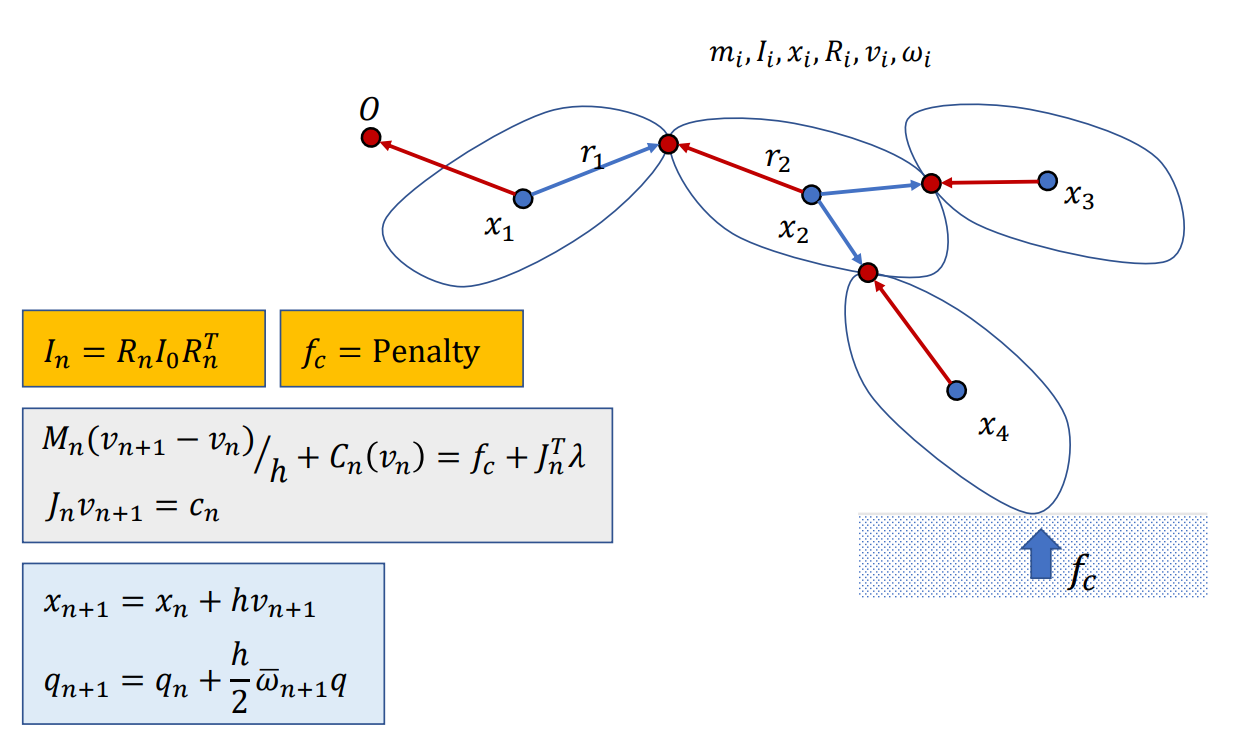
\includegraphics[totalheight=2in]{"./image/RigidBodySystem.png"}
  \caption{Rigid Body System} \label{fig:RigidBodySystem}
\end{figure}
首先(1.)根据刚体初始状态做初始化,若碰撞建模以Penalty方式建模,需要计算其接触力$f_c$的大小,
然后(2. 3.)构造运动学方程,其中关节的约束(3.)比较关键,对该运动学方程求解,可以得到
下一时刻的速度和角速度,最后分别对速度和角度做积分,得到新的位置,和新的旋转(四元数)信息。不断迭代,就完成了对一个
刚体系统的仿真。

需要注意的是,在上面的方程中,关节之间的主动力没有写上,这个力是使得角色运动的力,如何计算这个力,
将在下一节中说明。

\begin{problemset}
  \item 隐式积分的收敛性
  \item 什么是刚体动力学方程?
\end{problemset}

\chapter{角色控制}
\section{角色仿真和控制}
如何在一个物理引擎中定义刚体?通常我们需要定义如下参数:
\begin{enumerate}[itemindent=2em]
  \item 质量,转动惯量(Masses): $m, I$
  \item 位置,速度,朝向,角速度(Kinematics): $x, v, R, \omega$
  \item 几何(Geometry):
  \begin{enumerate}[itemindent=2em]
    \item Box,Sphere, Capsule, Mesh,\dots
    \item Collision detection
    \item Compute $m, I$
  \end{enumerate}
\end{enumerate}

\begin{figure}[htbp]
  \centering
  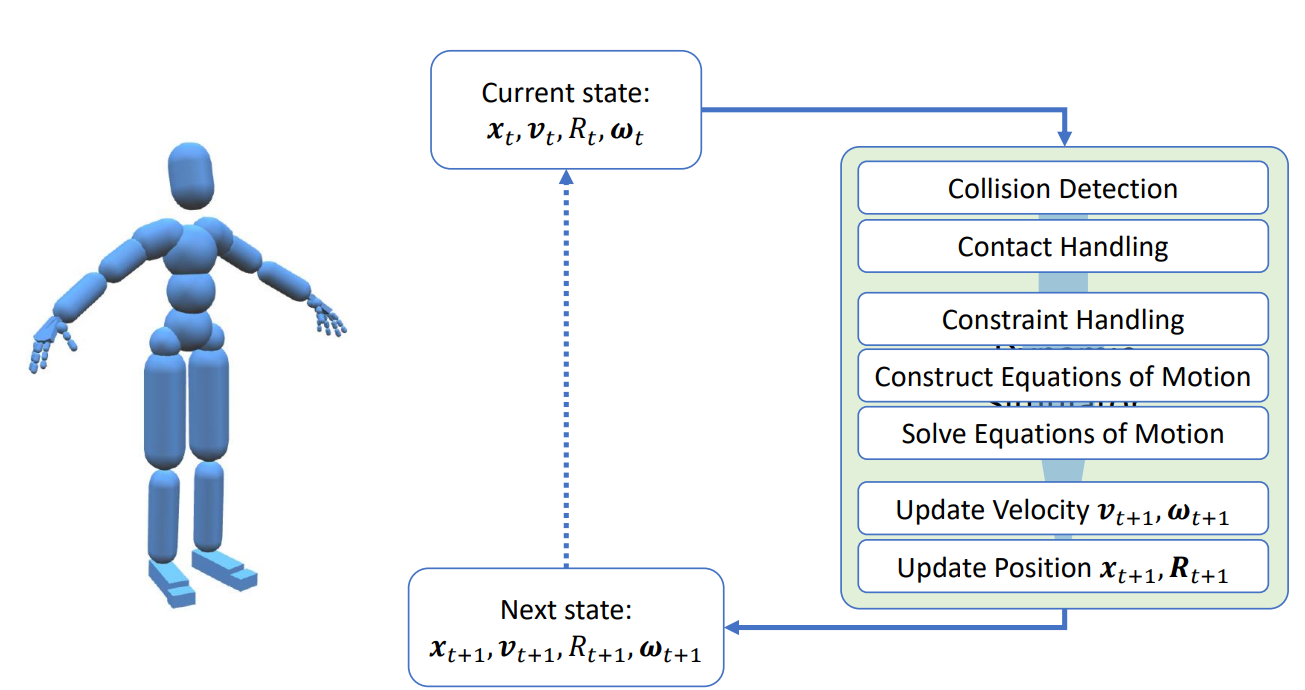
\includegraphics[totalheight=2.5in]{"./image/SimulatingCharacter.png"}
  \caption{Simulating a Character} \label{fig:SimulatingCharacter}
\end{figure}
若直接把物体采用图\ref{fig:SimulatingCharacter}的方式建立在仿真器中,物体将会瘫在地上Rogdoll,
虽然角色的动作是物理真实的,但因为缺乏控制,只能在重力的作用下,瘫在一起。

为了让一个角色(刚体)如我们希望的样子运动,需要给它施加一个外力。这就是物理仿真和关键帧动画的最大区别。
在关键帧动画中,我们希望角色处于什么状态,直接将该角色的状态,位置设置成目标姿势就行,但物理仿真不能直接
设置,只能通过在每个刚体上加上合适的力和力矩,这些力和力矩体现在运动方程中,会改变每一个刚体的速度和加速度,
从而进一步影响角色的动作。通常而言对刚体施加的各种力会综合到施加在质心上的一个力,力矩的效果上。
对一个真实的物体,不可能施加一个力矩,可以近似理解为一对大小相等,方向相反的力。

为了让一对刚体运动,可以在关节上加上一个力矩(joint torque,$\tau$),称为关节力矩。而关于关节力矩(Joint Torques)的含义,需要多说几句。
一是什么是关节力矩,二是如何作用关节力矩。
首先运动约束方程\ref{constrain::eqjoint}中运动部分没有关节,约束$Jv=0$是关于关节的约束,
而关节力矩本质上是在关节上施加的力矩,运动方程中起作用的力$f,\tau$都加在刚体上。所有现在的问题是,在关节
上加了力矩,这个力矩是如何加在它所对应的两个刚体上?

关节力矩是一个近似,一个机械臂的运动可由电机,马达来驱动,驱动带来的旋转效果,就是力矩。这个力矩往往
是多个力$\sum_i f_i = 0$的综合效应,多个合力为0的力,在关节上产生一个大小为$\tau$的力矩,该力矩
最终效果是在两个连接的刚体上,分别产生$\tau, -\tau$的力矩。
\begin{figure}[htbp]
  \centering
  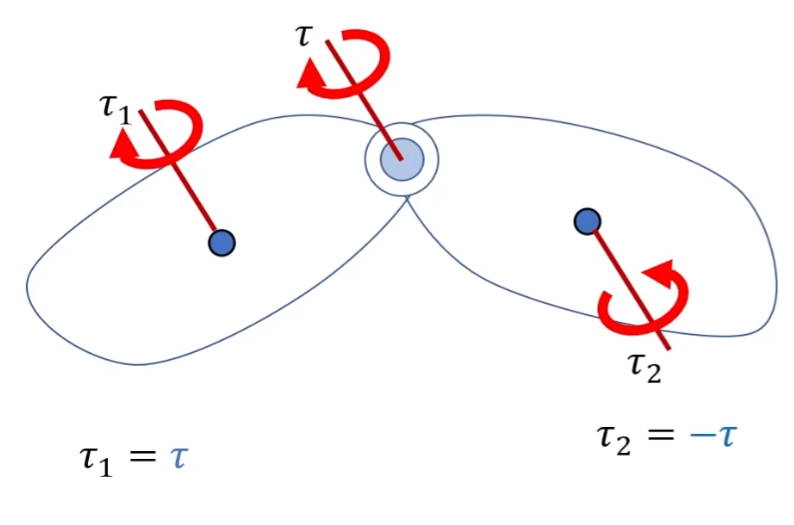
\includegraphics[totalheight=1.5in]{"./image/taujoint.png"}
  \caption{关节力矩} \label{fig:tau joint}
\end{figure}
在方程上,可表示为
\begin{equation}
  \begin{aligned}
  M\left[\begin{array}{c}
  \dot{v}_1 \\
  \dot{\omega}_1 \\
  \dot{v}_2 \\
  \dot{\omega}_2
  \end{array}\right]+\left[\begin{array}{c}
  0 \\
  \omega_1 \times I_1 \omega_1 \\
  0 \\
  \omega_2 \times I_2 \omega_2
  \end{array}\right] & =\left[\begin{array}{c}
  0 \\
  \tau \\
  0 \\
  -\tau
  \end{array}\right]+J^T \lambda \\
  J v & =0
  \end{aligned}
\end{equation}
表示对这个关节对应的两个刚体分别加了$\tau, -\tau$的力矩。

上面只是说明了在一个关节加了一个力矩,问题是怎么加?在实际环境中,由控制器
Controller来完成。
\begin{figure}[htbp]
  \centering
  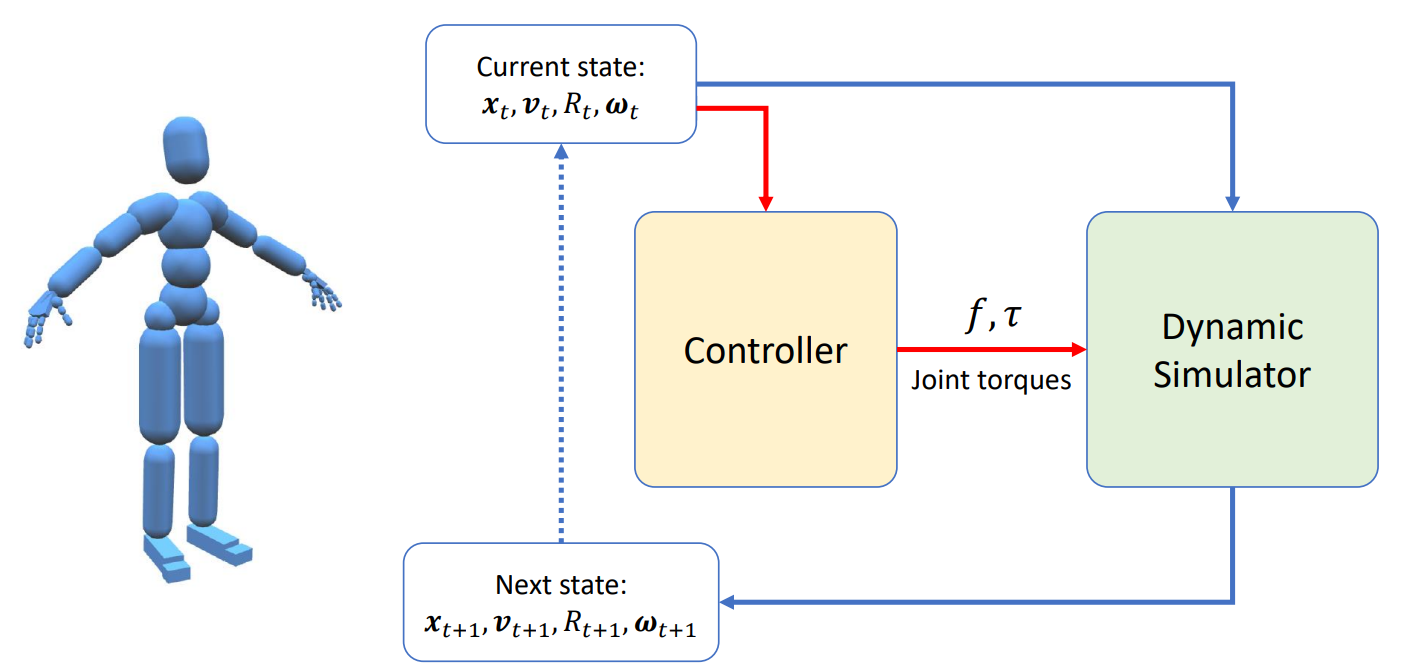
\includegraphics[totalheight=2.5in]{"./image/SimulatingControllingCharacter.png"}
  \caption{Simulating and Controlling} \label{fig:SimulatingControlling}
\end{figure}
控制器是根据角色当前的一些信息,位置,朝向,速度,角速度等,加上一些控制信号,比如走路到某地,
做什么动作,根据这些信息,实时计算每个关节的关节力矩,然后将这些关节力矩发送给仿真器,
产生最终的动作变化。

回看运动方程,$M \dot{\textcolor{blue}{\boldsymbol{v}}}+C(\boldsymbol{x}, \boldsymbol{v})  =
\textcolor{red}{\boldsymbol{f}}+\boldsymbol{J}^T \boldsymbol{\lambda}, J \boldsymbol{v} =0$
它是一个关于加速度和力的方程,这里就衍生出两个动力学概念:前向动力学,逆向动力学。
前向动力学是说给定力force/torques,计算加速度,即$[\boldsymbol{x}, \boldsymbol{v}, \textcolor{red}{f}]\mapsto \dot{\boldsymbol{v}}$。
逆向动力学是说给定加速度,计算力使得其产生这样的加速度,即
$[\boldsymbol{x}, \boldsymbol{v}, \textcolor{blue}{\dot{\boldsymbol{v}}}]\mapsto f$。

控制器根据角色的状态,计算每个关节的力矩,让角色动起来,其计算出来的关节力矩的总自由度(参数量),
和定义角色状态所需要的参数量有一些关系。如果驱动力$f,\tau$的总自由度比关节的自由度小,这种被称为
一个欠驱动(underactuated),若更大,则称为完全驱动fully-actuated。举例,机械臂是一个完全驱动系统,
人体是一个欠驱动系统。对于人体来说,其根关节是不固定的,不能直接更改根关节的性质,另外人体的关节比
刚体少一个,因此人体关节能提供的驱动数一定比刚体的状态自由度小。从另一个角度来说,人体在空间站中处于
失重状态,若没有外界力作用,人只能处于漂浮状态,驱动力缺少对人体全身的控制,或者从走路的角度来看,
人只能根据对地面施加力,根据地面的反作用力来控制人体质心的位置变化,从而移动,而不能直接控制质心的位置,来改变位置。

对于完全驱动系统,对任意加速度,都可以找到一个力,产生这样的加速度,而对于欠驱动系统,有很多加速度,
我们都没办法找到这样的力,达到该效果。这样看来,对于欠驱动系统来说,我们往往是希望其不要落入无法控制的状态
之下,而尽量保持在可以控制的状态中,比如怎么保持平衡,怎么走路等。
\begin{figure}[htbp]
  \centering
  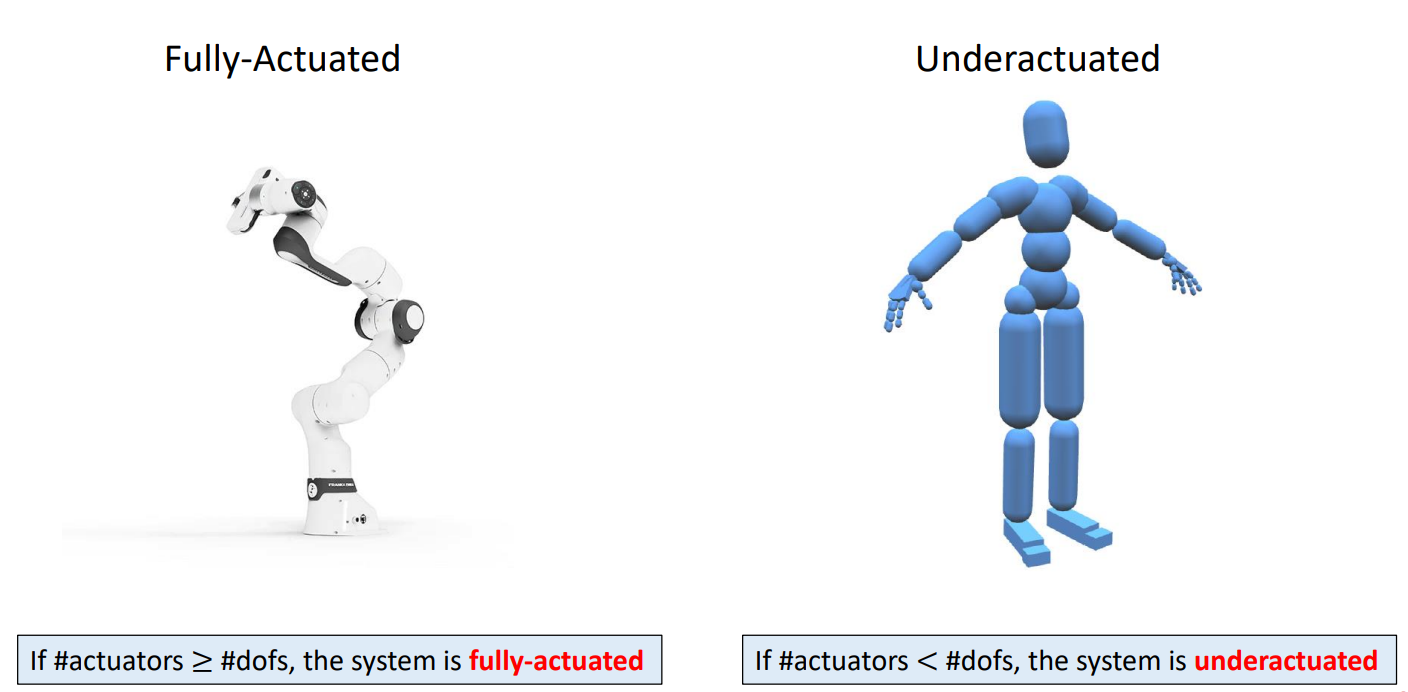
\includegraphics[totalheight=1.5in]{"./image/actuatedun.png"}
  \caption{actuated and unactuated} \label{fig:actuatedun}
\end{figure}

\section{前向、反馈、比例微分、轨迹追踪、雅可比转置等控制}
前向控制:执行预定义好的控制信号,没有考虑到当前角色的真实状态,若角色受到了扰动,
偏离了原计划的状态,是没办法修正回来,比如没有考虑到人在床上躺着,但是却一直执行向前
迈腿的动作,因此连站起来都不可能。反馈控制:
会根据当前角色的状态,去调整,使得其不会偏离正常范围,往往还希望受到扰动。
比例微分控制Proportional-Derivative Control(PD):通常是一个反馈控制。
\begin{figure}[htbp]
  \centering
  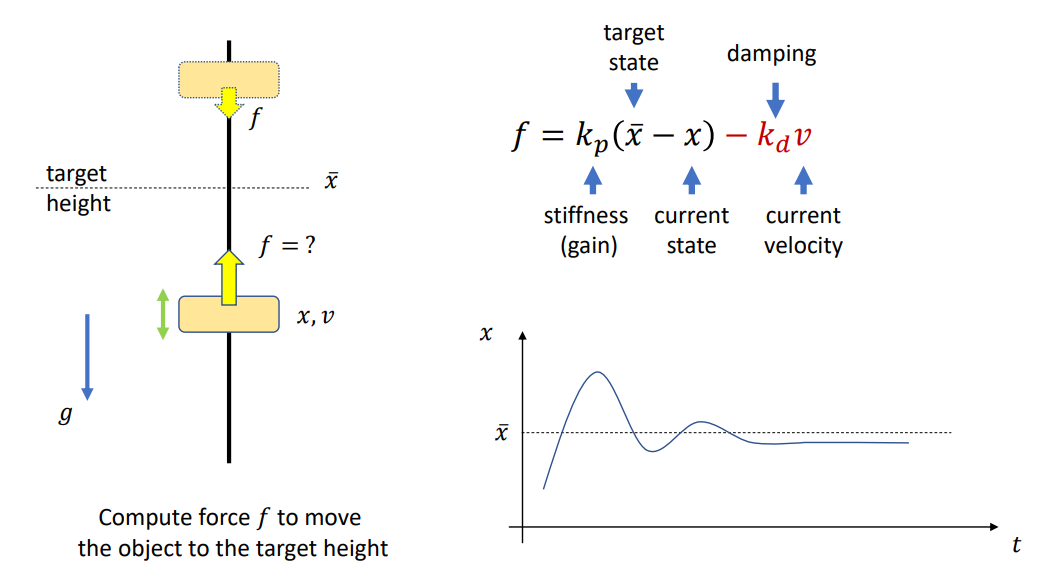
\includegraphics[totalheight=1.5in]{"./image/PDController.png"}
  \caption{PD Controller} \label{fig:PDController}
\end{figure}
比例微分在角色动画中,是一个前向控制,主要前向或反馈的看法是和控制目标有关系。

图\ref{fig:PDController} 中,控制器会根据物体当前的位置和速度,计算一个力,使其到达指定
位置(高度)。若重力加速度恒定,力的大小容易计算,否则计算更加麻烦。比例微分不是这样的思路。
它考虑当前位置和目标位置的偏差,根据偏差的大小来计算力的大小(线性拟合),也即比例控制$k_p$,
仅仅考虑这一个,容易想到,当物体到达指定目标时,物体会继续运动,然后$k_p<0$,使得最终
物体的运动轨迹程来回震荡的曲线,进而考虑速度,减去速度带来的继续运动效果,即微分控制$k_d$,可以理解为
阻尼,逐渐耗散掉原始能量。这样最终的运动轨迹呈现图右边的情况。公式也可以写为$f=k_p e + k_d \dot{e}$,
包含了位置误差控制和位置误差关于时间的微分控制。从图右边看到,比例微分最终效果所在位置和目标位置
有一点小的误差(分析略),该误差一般称为稳态误差Steady-state error,可以使用PID(Proportional-Integral-Derivative Control)去掉稳态误差,不过,
在动画领域,很少使用。该积分项和历史相关,在实现上存在一些额外的问题。所以实际应用中一般采用
将$k_p$设置的比较小的办法来减少稳态误差,但同时会带来系统的数值计算不稳定,以及物体动作很僵硬的效果。
不管怎么说,$k_p$一般不会设置得很大。另外$k_d$太小会震荡,太大会比较慢。

在角色控制中,$k_p$称为stiffness刚性参数,$k_d$称为dampping阻尼参数,图\ref{fig:CharacterPD}展示了对于一个刚体
做PD控制的逻辑。
\begin{figure}[htbp]
  \centering
  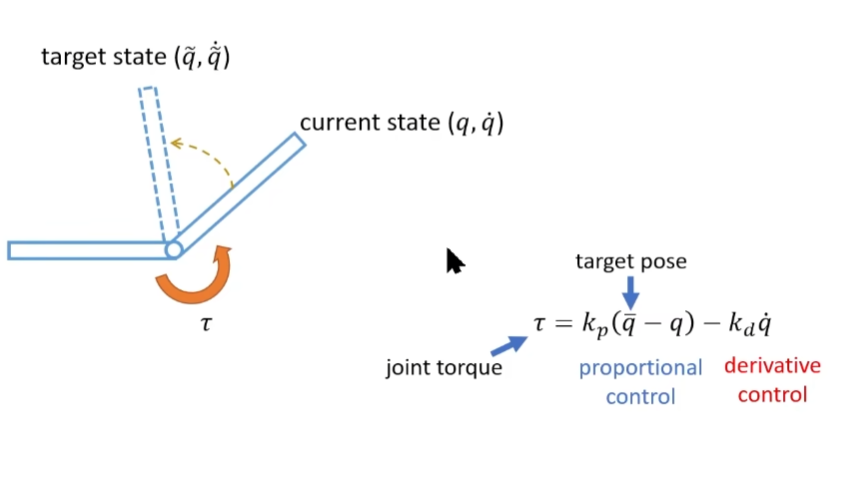
\includegraphics[totalheight=1.5in]{"./image/CharacterPD.png"}
  \caption{Character PD} \label{fig:CharacterPD}
\end{figure}

\begin{equation}
  \label{eq:PDCharacterJoint}
  \tau=k_p(\overline{\bar{q}}-q)+k_d(\dot{\bar{q}}-\dot{q})
\end{equation}
这里我们需要按照\ref{eq:PDCharacterJoint}计算每个节点的关节力矩,使得子关节到达旋转多少角度,到达
指定位置。自然而然,全身控制包含了对所有节点的控制,如图\ref{fig:FullCharacterPD}所示。实际经验告诉我们,
比如对于一个角色在任意状态到T-pose的转换,若stiffness太小,则无法达到指定目标T-pose,若太大,会很快到达指定
效果,但很僵硬。对于阻尼项dampping,若很小,就会有很明显的震荡,若很大,花费的时间会更长,但始终能达到指定
目标。
\begin{figure}[htbp]
  \centering
  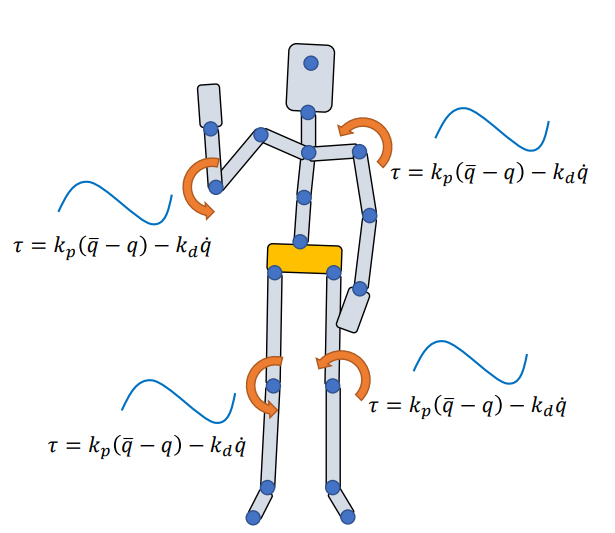
\includegraphics[totalheight=1.5in]{"./image/FullCharacterPD.png"}
  \caption{Full Character PD} \label{fig:FullCharacterPD}
\end{figure}

给出了一个PD控制后,控制本身变为了去设计一个轨迹,然后追踪这个轨迹。每一个关节设计一个轨迹,
就组成了全身跟踪\ref{fig:FullCharacterPD}。问题,如何去设计合理的轨迹?
\begin{figure}[htbp]
  \centering
  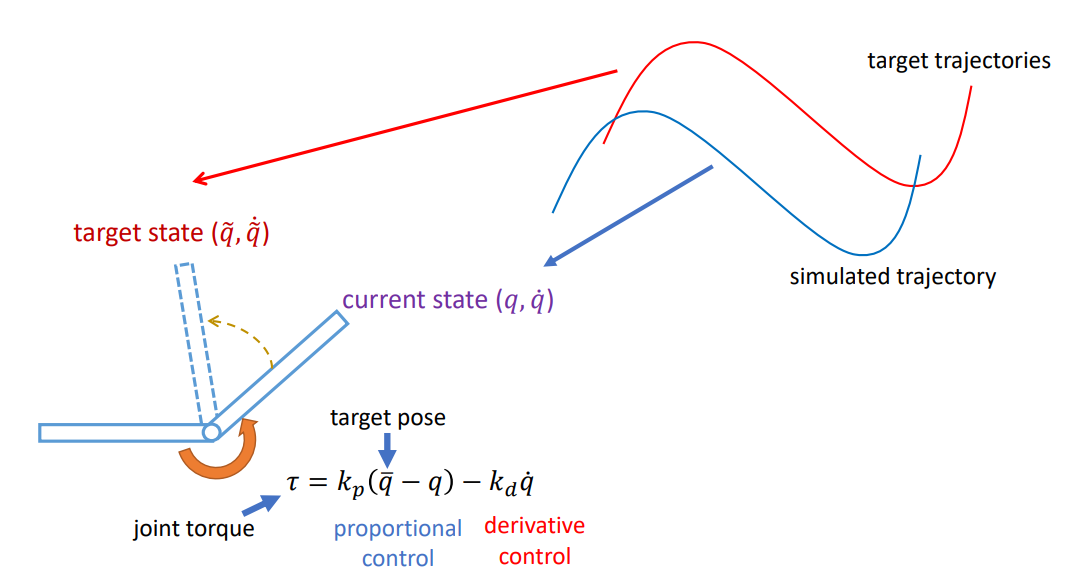
\includegraphics[totalheight=1.5in]{"./image/trajectoriesPD.png"}
  \caption{trajectories PD} \label{fig:trajectoriesPD}
\end{figure}
不过,实际设计出来的轨迹,用PD控制,往往会出现相位偏差问题,包括利用动捕数据,相位偏差导致
动作完成时间滞后,或不能完整完成,或者大体动作像,但不对。更进一步会导致,后续跟踪无法去修复
前面的误差。

PD控制是一个反馈控制,而对于走路来说,反而是一个前向控制,因为反馈本身是对关节的力矩的反馈,
但走路跟踪的状态实际是从一个目标轨迹上获取的,它和当前角色的状态没有关系。

以上跟踪会存在摔倒情况,原因在于没有对全局状态做跟踪。具体来说,对于关节$\tau_j$来说,
会给子节点施加一个$\tau_j$的力矩,对父节点施加一个$-\tau_j$的力矩,对全身来说,总体
力矩为0,因而无法改变全局(质心)朝向和位置。增加根节点力矩root force/torque是一个解决的方法。
这种方法,虽然能使物体保持平衡,但会使得角色看起来被某种东西拽着,呈现一种非物理真实的效果,
主要原因在于根关节没有父节点,施加在上面的力,实际会作用到全身。

在没有这些外力的情况下,如何使角色受控制,呈现一个平衡的效果?

\subsection{更稳定的PD控制}
一个简易的弹簧系统,就是一个PD控制系统。
具体来说,质量,位置,速度分别为$m,x,v$的弹簧,进度系数,阻尼系数$k_p,k_d$,为了方便起见,设目标值为0,
则有$f=-k_p x - k_d v$。设步长为$h$,其半隐式欧拉积分(用更新之后的速度去更新位置)为:
\begin{equation}
  \begin{aligned}
  & v_{n+1}=v_n+h \frac{f}{m} \\
  & x_{n+1}=x_n+h v_{n+1}
  \end{aligned}
\end{equation}
假设$m=1$,带入$f$,写为矩阵形式:
\begin{equation}
  \begin{gathered}
  {\left[\begin{array}{l}
  v_{n+1} \\
  x_{n+1}
  \end{array}\right]=\left[\begin{array}{cc}
  1-k_d h & -k_p h \\
  h\left(1-k_d h\right) & 1-k_p h^2
  \end{array}\right]\left[\begin{array}{l}
  v_n \\
  x_n
  \end{array}\right]} \\
  \boldsymbol{s}_{n+1}=A \boldsymbol{s}_n \\
  \boldsymbol{s}_{n+1}=A^n \boldsymbol{s}_1
  \end{gathered}
\end{equation}
这里假设$A$有两个特征值,$\lambda_1, \lambda_2,\in \mathbb{C}$
于是有$A=P diag(\lambda_1, \lambda_2)P^{-1}$。

对$P$做变换,$z=P_{-1}s$,则$z_{n+1}=diag(\lambda_1, \lambda_2)z_n$,这里$s$为上面的矩阵$s_i$。
于是上面矩阵关系可重新写为:$z_{n+1}=diag(\lambda_1, \lambda_2)^n z_1$。

容易得到$|\lambda_1|>1 \Rightarrow \lim_{x \to \infty}\|z_n\| \rightarrow \infty$,即系统不稳定。
也就是为了保证仿真系统稳定,需要$A$的特征值都小于1。具体到$k_p,k_d,h$的关系,需要根据实际的数据,模拟出来,
以确定$h$应该选取的范围。一般对于一个50kg的角色,可以设置$k_p = 200, k_d = 20$,在实际中可能存在几百步长以后,
系统就不稳定,此时可能$h=0.5\thicksim 1ms, 1000\thicksim 2000Hz$,但$h$太小,意味着每一秒中需要计算更多次
的计算,会带来运算量的增加。如何解决系统不稳定的问题?

将PD控制的某一部分(速度)变为隐式欧拉表达(可大大增加仿真系统的稳定性),
此时系统方程变为:
\begin{equation}
  \label{eq:stablepd}
  \begin{aligned}
  & v_{n+1}=v_n+h (-k_{p}x_n - k_{d}v_{n+1}) \\
  & x_{n+1}=x_n+h v_{n+1}
  \end{aligned}
\end{equation}
矩阵形式为:
\begin{equation}
  \left[\begin{array}{l}
  v_{n+1} \\
  x_{n+1}
  \end{array}\right]=\frac{1}{1+h k_d}\left[\begin{array}{cc}
  1 & -k_p h \\
  h & 1+k_d h-k_p h^2
  \end{array}\right]\left[\begin{array}{l}
  v_n \\
  x_n
  \end{array}\right]
\end{equation}

通常用显式的PD,可能需要很小的步长,1/1000秒,如果用stable PD(\ref{eq:stablepd}),则能使用
更长的步长。通常来说,一个仿真系统,控制部分能做到120Hz,一般就是stable PD。

\subsection{轨迹优化}
使用动捕数据,会存在跟踪不上的问题,对于给定的轨迹,若沿着直接到目标的轨迹,也存在同样的问题。
如何找到控制轨迹,使得能跟踪上,不存在偏差?可以在已有的轨迹上,做新的设计,或者轨迹优化
Trajectory Optimization。

找到轨迹:
\begin{enumerate}[itemindent=2em]
  \item 仿真轨迹: $s_0, s_1, \ldots, s_T$
  \item 控制轨迹:$a_0, a_1, \ldots, a_{T-1}$
  \item 最小化目标函数:$$\min _{\left\{s_t, a_t\right\}} f\left(s_T\right)+\sum_{t=0}^{T-1} f\left(s_t, a_t\right)$$
  \item 同时满足限制:
  $$
  \begin{aligned}
  M \dot{v}+C(\boldsymbol{x}, \boldsymbol{v}) & =\boldsymbol{f}+J^T \lambda & & \text {运动方程} \\
  g(\boldsymbol{x}, \boldsymbol{v}) & \geq 0 & & \text { 限制条件 }
  \end{aligned}
  $$
\end{enumerate}
其中目标函数$f(s_T)$表示轨迹结束时的状态,以及求和部分表示每一时刻,加了多少力和当前的状态。
而约束是因为角色运动需要对当前的状态施加力,根据仿真,得到下一时刻的状态。状态$s_i$和力$a_i$
之间是存在运动方程限制的,$g$表示其他可能的约束,比如关节约束,角色不能走到悬崖的边上(位置约束)。

举个例子,对图\ref{fig:CharacterPD}中滑杆运动,希望其运动轨迹为$\sin$函数,此时目标轨迹应该为什么?
沿用上面找轨迹的建模思路有:
\begin{equation}
  \begin{array}{ll}
  \min _{\left\{x_n, v_n, \bar{x}_n\right\}} & \sum_{n=0}^N\left(\sin \left(t_n\right)-x_n\right)^2+w_{\bar{x}} \sum_{n=0}^N \bar{x}_n^2 \\
  \text { s.t. } & v_{n+1}=v_n+h\left(k_p\left(\bar{x}_n-x_n\right)-k_d v_n\right) \\
  & x_{n+1}=x_n+h v_{n+1}
  \end{array}
\end{equation}
这里$\sum_{n=0}^N \bar{x}_n^2$为一个位置正则项,限制其值比较小,使得轨迹比较平滑。限制条件s.t中,在优化领域被称为
硬约束,需要两边一定相等,软约束即为两边约等就行,可写为如下:
\begin{equation}
  \begin{aligned}
  \min _{\left.c_n, v_n, \bar{x}_n\right\}} & \sum_{n=0}^N\left(\sin \left(t_n\right)-x_n\right)^2+w_{\bar{x}} \sum_{n=0}^N \bar{x}_n^2 \\
  & +w_v \sum_{n=0}^N\left(v_{n+1}-v_n-h\left(k_p\left(\bar{x}_n-x_n\right)-k_d v_n\right)\right)^2 \\
  & +w_x \sum_{n=0}^N\left(x_{n+1}-x_n-h v_{n+1}\right)^2
  \end{aligned}
\end{equation}
式中约束部分的权重参数$w_v,w_x$刻画了软的程度,越大越硬,极限情况极为硬约束。

在实际工作中,会面临上面优化目标的参数太大的问题,对于这种情况,还有一种被称为Collocation method的方法,
它优化的不是实际的参数,对给定目标轨迹,同时优化一系列带参数的曲线,而曲线本身往往是多项式
或样条曲线,优化曲线转化为优化样条等曲线的参数,从而达到参数降维的目的。
具体优化目标可表达为:
\begin{equation}
  \begin{aligned}
  & \min _{\left\{x_n, v_n, \bar{x}_n\right\}} \sum_{n=0}^N\left(\sin \left(t_n ; \theta\right)-x\left(t_n ; \theta\right)\right)^2+w_{\bar{x}} \sum_{n=0}^N \bar{x}^2\left(t_n ; \theta\right) \\
  & \text { s.t. } \quad \begin{aligned}
  v\left(t_{n+1} ; \theta\right) & =v\left(t_n\right) \\
  & +h k_p\left(\bar{x}\left(t_n ; \theta\right)-x\left(t_n ; \theta\right)\right)-h k_d v\left(t_n ; \theta\right) \\
  \qquad x\left(t_{n+1} ; \theta\right) & =x\left(t_n ; \theta\right)+h v\left(t_{n+1} ; \theta\right)
  \end{aligned}
  \end{aligned}
\end{equation}
其中优化参数为${x_n, v_n, \bar{x}_n}$。

常见的优化方法:梯度下降,牛顿法,拟牛顿法。但对于上面这个问题,是一个典型的二次型问题,
可以具体解出来。

而在实际工作中,我们会面临优化问题常常是高度非线性的,比如角色运动,具体计算的时候,系统是一个黑盒子,无法得到具体
的梯度值,或者高维曲离散面震荡明显,梯度不可靠等问题。另一方面,很多情况,我们都很难对运动本身做准确的建模,比如人手
的软的,拿筷子很容易,但在仿真系统中,用刚体拿筷子,就比较麻烦。这种时候,没具体模型,无法计算梯度。
因此,基于梯度的优化算法,也有它的局限性。无法利用梯度优化的问题,可以选择启发式方法。

非梯度优化的迭代方法:
\begin{enumerate}[itemindent=2em]
  \item 目标:找一个变量$\boldsymbol{x}$最小化$f(\boldsymbol{x})$
  \item 首先初始化$\boldsymbol{x}$(角色跟踪动捕数据,动捕数据本身可作为初始估计)
  \item 迭代:
  \begin{itemize}[itemindent=2em]
    \item 根据当前估计$\boldsymbol{x}$,生成一些样本点${\boldsymbol{x_i}}$
    \item 计算每个样本点的函数值$f_i = f(\boldsymbol{x_i})$
    \item 更新$\boldsymbol{x}$的估计
  \end{itemize}
\end{enumerate}
有贝叶斯优化,进化算法(CMA-ES),随机优化,蒙特卡洛序列等。

缺点:随机采样,通过若干样本点,来更新,速度慢,精确性比较比较差。

\subsubsection{CMA-ES}
[Hansen 2006, The CMA evolution strategy: a comparing review]。
对于黑盒子也可以使用,并且有些比较复杂的动作,也能有较好的效果。
\begin{figure}[htbp]
  \centering
  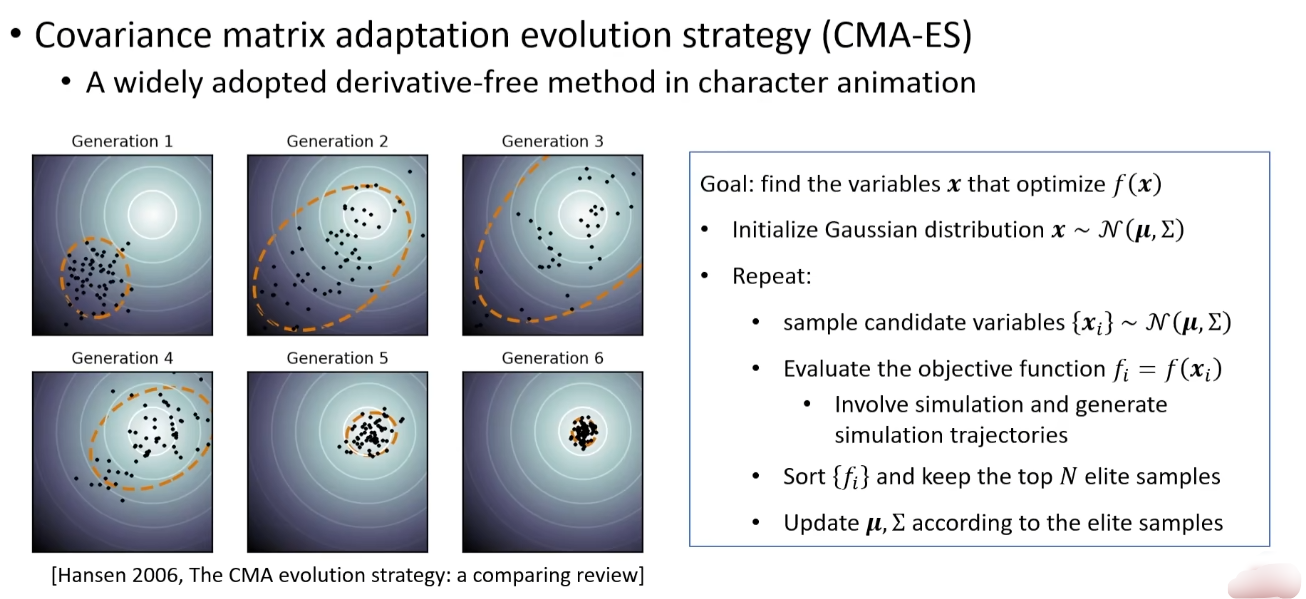
\includegraphics[totalheight=1.5in]{"./image/CMA-ES.png"}
  \caption{CMA-ES} \label{fig:CMA-ES}
\end{figure}
CMA-ES每次对给定参数,都需要做仿真,过程比较漫长,若仿真的轨迹比较长,
就更难收敛。

其他略。
\subsubsection{SAMCON}
SAmpling-based Motion CONtrol [Liu et al. 2010, 2015],
对动捕数据的轨迹跟踪。每次采样,只考虑下一帧,即优化一步。
本质是一个序列蒙特卡洛方法。
\begin{figure}[htbp]
  \centering
  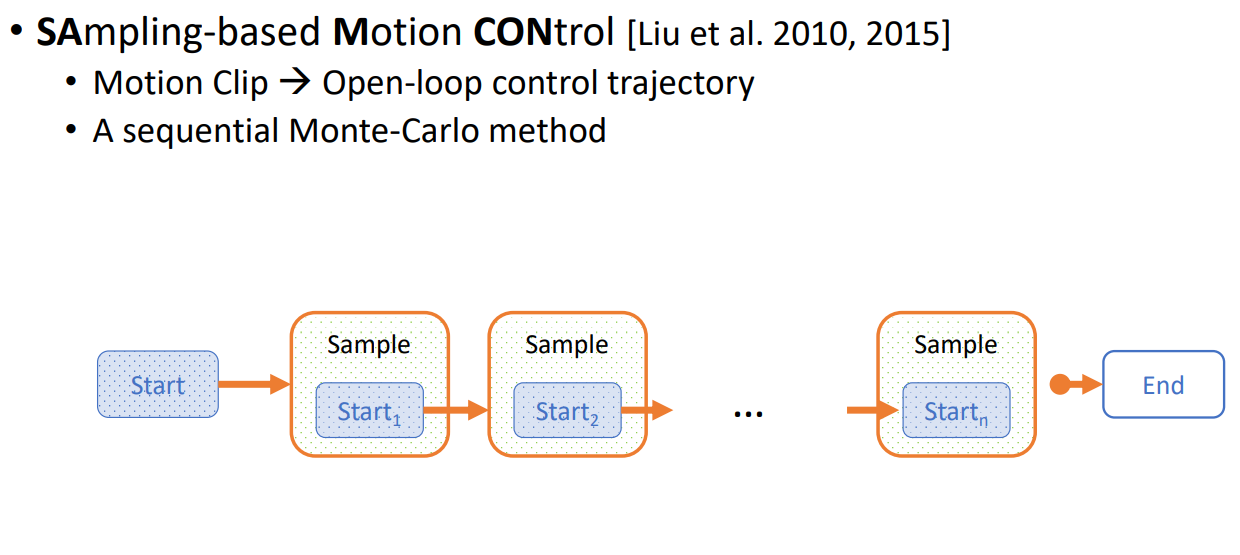
\includegraphics[totalheight=1.5in]{"./image/SAMCON.png"}
  \caption{SAMCON} \label{fig:SAMCON}
\end{figure}

从初始状态开始,采一些样本点做仿真,从仿真的结果中取出
一小部分作为新的出发点,再采样,以此类推。

其他略。
\subsection{反馈控制}
在前向控制中,对给定轨迹,若加一点扰动,角色会快速偏离原始轨迹,为了解决这个
问题,需要引入反馈控制,即每一时刻有一个反馈的策略,这个策略会自动根据当前状态
进行更新(根据原始状态和扰动状态的偏差),这样保持运动在原始轨迹附近。这样每一步
就会有相应的反馈策略。
\subsubsection{Static Balance}
静态平衡,让PD控制的目标是一个T-pose,去跟踪一个单一的姿势,角色虽然能保持住跟踪的姿势,
但会逐渐趋于摔倒状态。这就是缺少一个反馈控制,在角色将要摔倒的时候,将其更正回来。
比如让角色站立保持不动,可以使用左右摇晃,或者推一下,保持不摔倒,或者原地下蹲等,原点晃肩。

这里面有个关键概念:平衡。通常而言,静止物体的重心在地面的投影点在支撑面内,就可以保持平衡。
支撑面指物体于地面的接触面的凸包。比如人体,就是两脚所围住的面积。

用PD控制去计算一个反馈力矩:
\begin{equation}
  \label{eq:feedbackf}
\tau=k_p(\overline{\boldsymbol{c}}-\boldsymbol{c})-k_d \dot{\boldsymbol{c}}
\end{equation}

其中$\dot{\boldsymbol{c}}$表示质心的速度,$\overline{\boldsymbol{c}}$表示支撑平面的中心。
对于保持某种姿势的角色来说,其已经有其他的关节力矩来做
这件事,要让角色保持平衡,可在其他关节(踝关节,髋关节)上施加上面的力矩,使得质心的投影点在支撑面内。
除了PD控制策略,还可以使用雅可比转置控制。

\subsection{Jacobian Transpose Control}
\begin{figure}[htbp]
  \centering
  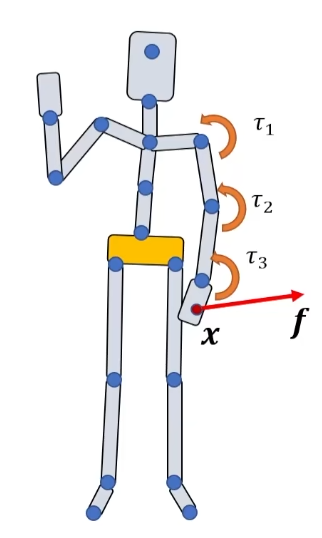
\includegraphics[totalheight=1.8in]{"./image/JacobianTransposeControl.png"}
  \caption{Jacobian Transpose Control} \label{fig:JacobianTransposeControl}
\end{figure}
Jacobian Transpose Control 雅可比转置控制:用关节力矩来等价的实现
一个力的效果。这个力并没有真正加在关节上,因此也被称为虚力。具体效果可以用做功来衡量:
功率=力*速度=力矩*角速度。本质来说就是IK问题,通过对前向运动学进行求导来得到。即
$P=\boldsymbol{f}^{T}\dot{\boldsymbol{x}}=\boldsymbol{\tau}^{T}\dot{\boldsymbol{\theta}},$
前向动力学$\boldsymbol{x}=g(\boldsymbol{\theta})\Rightarrow \dot{\boldsymbol{x}}=J\dot{\boldsymbol{\theta}},
J=\frac{\partial g}{\partial \boldsymbol{\theta}}$。
两者结合得到$\boldsymbol{f}^T J \dot{\boldsymbol{\theta}}=\boldsymbol{\tau}^T \dot{\boldsymbol{\theta}}$,
也即:
\begin{equation}
\boldsymbol{\tau} = J^T \boldsymbol{f}
\end{equation}
加力点$\boldsymbol{x}$的前向运动学的雅可比矩阵的转置乘以$\boldsymbol{f}$得到力矩。

进一步推导可得到如下结论:
\begin{equation}
  \tau_i=\left(x-p_i\right) \times f
\end{equation}
即每个关节的力矩等于关节点到加力点的向量叉乘力$\boldsymbol{f}$。

利用这个结论,可以改写上节中保持静态平衡所使用的PD控制方法。通过虚力的方式,
采用公式\ref{eq:feedbackf}来计算一个力,而非力矩。具体来说,假设力(非真实力,加不了
通过一些关节力矩实现类似的效果)加在质心上,使得质心被推到目标位置$\bar{\boldsymbol{c}}$。
类似的,用质心减去对应关节(髋关节,膝关节,踝关节)的位置,然后叉乘$\boldsymbol{f}$。
除此之外,目标$\bar{\boldsymbol{c}}$可以有高度,当高度降低,可以实现角色下蹲的效果。

但上面的方式,实现的平衡比较弱,能实现比较稳的站住,当有外力推角色的时候,力稍微大一点,可能就很难
保持平衡。

进一步工作参考:[Macchietto et al. 2009 - Momentum Control for Balance]。

\section{用简化模型学习走路}
前几节中,主要讲了如何仿真一个虚拟角色,如何控制一个角色,让角色保持一个姿势,如何利用反馈控制,
来保持原地的静态平衡,也能让角色在平衡中,做一些简单的动作。基本上是动捕数据的一个跟踪效果,动作本身所
涉及的很多细节并没有考虑进去,这些细节用纯粹的基于运动学的方式难以实现,比如人在挥手的时候,
手上的角动量会变化,身体会反抗,就会有一些微弱的摇晃。

除了站在原地平衡之外,这一节主要讲怎么走路。移动在运动学上,基于运动合成的方法,给角色设置合
适的姿态(位置变化别太远)就可以移动了。但基于物理学(动力学)的方法,我们不能控制一个角色的全局位置,
只能通过让角色和地面的交互,让地面的反作用力来驱动角色运动。

粗略来说,在2000年的前十五年中,基于仿真的角色动画方向研究的主要内容就是走路。走路难度还是挺大的。

Static Balance 只能实现比较慢的走路,单单考虑质心,来保持身体
的平衡,更加丰富的走路,需要考虑角动量。

本节主要涉及下面三篇文章:
\begin{itemize}[itemindent=2em]
  \item ZMP(Zero-Moment Point)
  \item Inverted Pendulum Model(2010)
  \item SIMBICON(Simple Biped locomotion Control, 2007)
\end{itemize}

简化模型:找到最能影响角色平衡的量,比如质心,来构建一个抽象模型。

Simplify humanoid / biped robot into an abstract model
\begin{itemize}[itemindent=2em]
  \item Often consists of a CoM and a massless mechanism
  \item Need to map the state of the robot to the abstract model
\end{itemize}

Plan the control and movement of the model
\begin{itemize}[itemindent=2em]
  \item Optimization
  \item Dynamic programming
  \item Optimal control
  \item MPC
\end{itemize}

Track the planned motion of the abstract model
\begin{itemize}[itemindent=2em]
  \item Inverse Kinematics
  \item Inverse Dynamics
\end{itemize}

\subsection{Zero-Moment Point}
当人在走路时,如\ref{fig:ZMP-GRF}所示,可将脚所受的力分解如右边小图。
\begin{figure}[htbp]
  \centering
  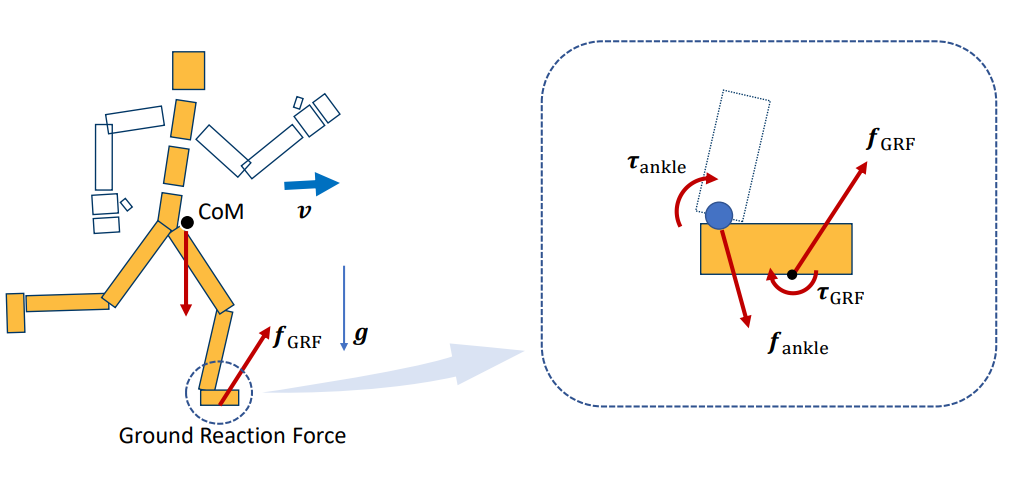
\includegraphics[totalheight=1.6in]{"./image/ZMP-GRF.png"}
  \caption{ZMP-GRF} \label{fig:ZMP-GRF}
\end{figure}
上半身的移动,主要也就是踝关节处所施加的力。对于脚来说,是一个脚平面与大地平面
的相互作用。对于脚平面上的任意点$p_i$,其有地面力$f_i$,可分解为$f^y _l + f^{xz} _l$,
分别称为支持力,摩檫力。对于脚平面上的所有点的力分析,等价于对某一个点$p$的力分析。
按照前面对刚体的处理方式,假设地面是平整的且脚面点到点$p$是在同一水平面上,则
有$\tau_{GRF}=\sum_{i}(p_i - p)\times f_i$。由$f_i$的分解,
有
\begin{equation}
  \begin{aligned}
  \boldsymbol{\tau}_{\mathrm{GRF}} & =\sum_i\left(\boldsymbol{p}_i-\boldsymbol{p}\right) \times\left(f_i^y+f_i^{x z}\right) \\
  & =\sum_i\left(\boldsymbol{p}_i-\boldsymbol{p}\right) \times f_i^y+\sum_i\left(\boldsymbol{p}_i-\boldsymbol{p}\right) \times f_i^{x z}
  \end{aligned}
\end{equation}
得到力矩在水平(平行)和竖直(垂直)两个方向上的分解。这里$P$可任意选择,水平向的力具有旋转效果,
我们可以选择一个点,使得$\tau_{GRF}^{xz}=0$。该点被称为Center of Pressure,解算方程,容易得到
$\mathrm{p}=\frac{\sum_{i}\mathrm{p_i}\mathrm{f_i}^y}{\sum_{i}\mathrm{f_i}^y}$
$\Rightarrow \tau_{\mathrm{GRF}}^{xz}=0$,
如此选点(Center of Pressure),可只关心竖直方向上的力。

在水平方向上,所有力,力矩作用在脚上,使得脚在水平上保持不移动,因此有静态等式:
$f_{ankle} + f_{GRF} + mg = 0$,同时关于参考点$o$的动量也有:$(u -o)\times f_{ankle} + (p-o)\times f_{GRF}
+ (x-o)\times mg + \tau_{GRF}^{y} + \tau_{ankle} = 0 $,
参数相关含义参考图\ref{fig:ZMP-stance-phase}。
\begin{figure}[htbp]
  \centering
  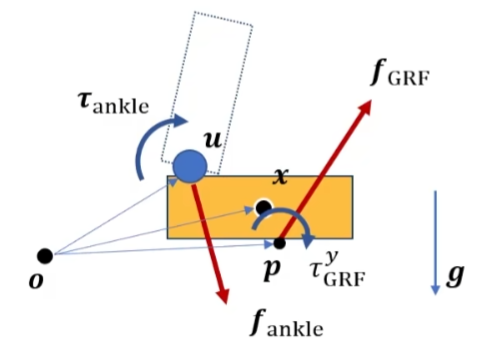
\includegraphics[totalheight=1.6in]{"./image/ZMP-stance-phase.png"}
  \caption{ZMP stance phase} \label{fig:ZMP-stance-phase}
\end{figure}
若只考虑水平方向,则上式去掉$\tau_{GRF}^{y}$,将力$f$映射到水平面$xz$,从而有
\begin{equation}
  \begin{array}{r}
  \left((\boldsymbol{u}-\boldsymbol{o}) \times \boldsymbol{f}_{\text {ankle }}\right)^{x z}+\left((\boldsymbol{p}-\mathbf{o}) \times \boldsymbol{f}_{\mathrm{GRF}}\right)^{x Z} \\
  \quad+(\boldsymbol{x}-\boldsymbol{o}) \times m \boldsymbol{g}+\boldsymbol{\tau}_{\text {ankle }}^{x z}=\mathbf{0}
  \end{array}
\end{equation}
上式中,$x$是脚掌的质心,已知$u, o, x,f_{*}$,则$p$点可计算出来$(?,?,0)$。
点$p$被称为零力矩点(Zero-Moment Point, ZMP),因为它假设了旋转力矩$\tau_{GRF}^{xz}=0$,
同时和力矩的水平分量也等于$0$。

零力矩点成立的条件是$p$在支撑面(support polygon)内。

如果人正处于摔倒状态,上面计算得到的$p$点,将在支撑面的外面,此时
$\tau_{\mathrm{GRF}}^{xz} \neq 0$。此时水平方向的合外力矩不为0,
会让脚向外反转,抬起来,使人更容易摔倒。

总的来说,ZMP是一个指标,只要能保证$p$点在支撑面内,就可以实现让角色处于动态平衡的状态。
但是如何控制ZMP就相对比较复杂,需要较大篇幅,比如一门课,才能说明白。

ZMP控制移动得比较慢,它假设脚掌与地面平行,对机器人来说,需要让膝盖弯曲,来控制零力矩点
在支撑面内。
\subsection{Inverted Pendulum Model}
IPM称为倒立摆模型:轴在地下,物体在顶部,受重力影响,向下旋转移动。从图\ref{fig:IPM}可
得到$\ddot{\theta}=\frac{g}{\ell} \sin \theta$。
\begin{figure}[htbp]
  \centering
  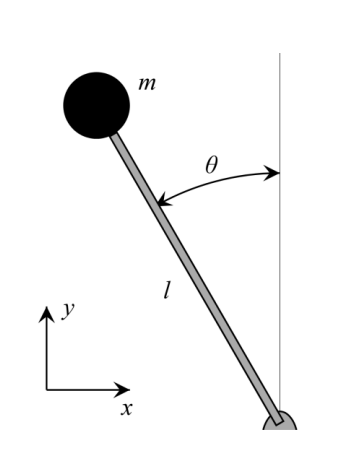
\includegraphics[totalheight=1.6in]{"./image/IPM.png"}
  \caption{IPM} \label{fig:IPM}
\end{figure}
控制过程,由在轴部位移动来控制。比如轴底加一辆小车,杆往左下滑动,车就往左边移动。
比如把扫帚放在手指上保持扫帚的平衡就是IPM控制。

这里简单介绍一篇比较经典的使用IPM思路来控制角色的工作:[Coros et al. 2010 - Generalized Biped Walking Control]。

结合图\ref{fig:IPM-Control}来说明该文章的主要思路:
\begin{itemize}[itemindent=2em]
  \item 将角色的质心和站立脚映射为IPM(重心到支撑点的连线构成倒立摆),人在摔倒的时候,
  速度会越来越大
  \item 通过当前质心的速度,计算下一个脚步的位置,使质点位于摆的顶部,此时刚好稳定,速度为$0$,
  \item 脚当前位置和之前的位置,可以使用样条插值,做一个脚部轨迹
  \item 使用 IK 计算目标姿势(通过质心和脚的位置算出一个目标姿势,通过PD控制,实现对角色的控制)
\end{itemize}

\begin{figure}[htbp]
  \centering
  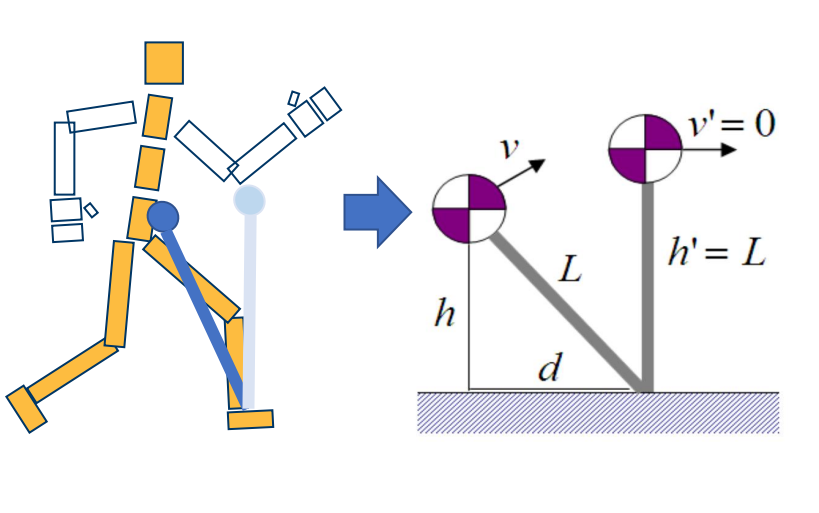
\includegraphics[totalheight=1.6in]{"./image/IPM-Control.png"}
  \caption{IPM Control} \label{fig:IPM-Control}
\end{figure}

根据能量守恒定律,动能转化为势能,可以得到如下关系:
\begin{equation}
  \begin{aligned}
  & \frac{1}{2} m v^2+m g h=\frac{1}{2} m v^{\prime 2}+m g h^{\prime} \\
  & v^{\prime}=0 \text { and } h^{\prime}=L=\sqrt{h^2+d^2} \\
  & d=v \sqrt{h / g+v^2 /\left(4 g^2\right)} .
  \end{aligned}
\end{equation}
得到脚步长$d$。

该方法比较通用,鲁棒,在转化为IK去计算姿势这一块,比较复杂。

\subsection{SIMBICON}
文章[SIMBICON:SIMple BIped Locomotion CONtrol. Yin et al. 2007]
第一个实现了比较鲁棒的步行控制,可以通过非常简单的反馈,实现步行控制。
主要思路可以简单理解为跟踪控制+反馈。

具体的略。

该方法动作质量上稍微有点不尽人意。

\begin{problemset}
  \item 实现一个站立控制,包含PD Control,Hand of God,Static Balance
  \item 实现走路控制器(Bonus)
  \item 简化模型基本都是在走路的基础上建立起来的,很难迁移到其他动作上,对于更广泛的动作如何实现控制?
  甚至生成新的动作。(强化学习对控制策略的学习,会带来更好的效果,但可解释性比较差)
\end{problemset}

\chapter{最优控制和强化学习}
本章从与强化学非常相关的理论最优化控制出发,来说明强化学习和传统方法的一些区别。
\section{最优控制}
前面讲到,通过对角色施加力和力矩,来控制角色,实现对角色的驱动。比如需要做一个后空翻,
需要找到一些自动控制策略,比如PD target,然后去执行这个PD target让角色的仿真轨迹
和目标轨迹相同。为了找到这些轨迹,可以把控制建模成优化问题。在每一帧,都可以计算当前帧
和参考数据的偏差,将这些偏差加起来,就构成了一个优化问题。优化的对象是每一帧需要施加的力。
在具体的仿真过程中,需要每一步都满足简化的物理规律。

具体来讲就是找到一组控制序列${a_t}$从初始状态$s_0$开始,生成状态序列${s_t}$,
最小化目标函数
\begin{equation}
  \label{eq:trajectory}
  \min h\left(s_T\right)+\sum_{t=0}^{T-1} h\left(s_t, a_t\right)
\end{equation}
使得对$[0, T]$中所有时间,满足$f(s_t, a_t) - s_{t+1} = 0$。同时角色本身满足运动方程:
\begin{equation}
  \label{eq:trajectorycontrol}
  \begin{gathered}
  M \dot{\boldsymbol{v}}+C(\boldsymbol{x}, \boldsymbol{v})=\boldsymbol{f}+J^T \lambda \\
  g(\boldsymbol{x}, \boldsymbol{v}) \geq 0
  \end{gathered}
\end{equation}

若只优化轨迹,称为开环控制,或者前馈控制。
前馈控制:根据一些预定义的控制策略做修改,不根据状态的改变而改变。因此对于扰动,就比较困难。

\begin{figure}[htbp]
  \centering
  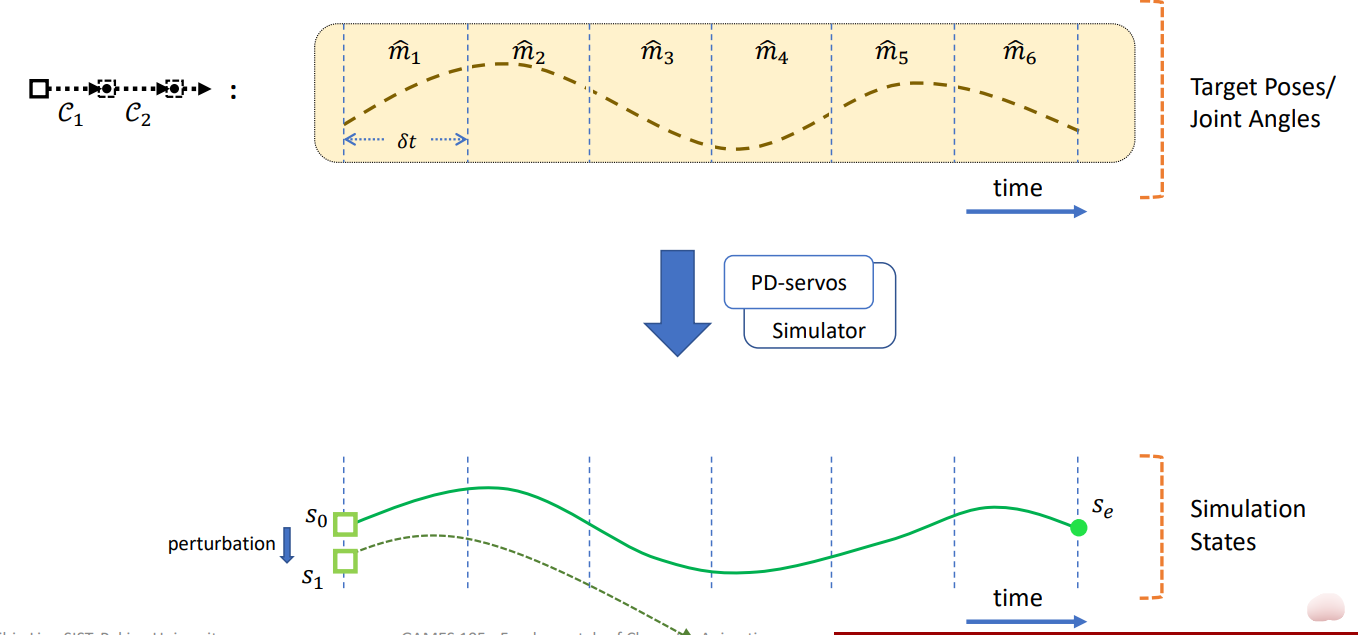
\includegraphics[totalheight=1.6in]{"./image/Feedforward-Control.png"}
  \caption{Feedforward Control} \label{fig:Feedforward-Controll}
\end{figure}

反馈控制:根据当前角色受到扰动之后的状态,更新控制策略(信号?)的变化,从而保证角色在控制过程
中能经得起干扰。
\begin{figure}[htbp]
  \centering
  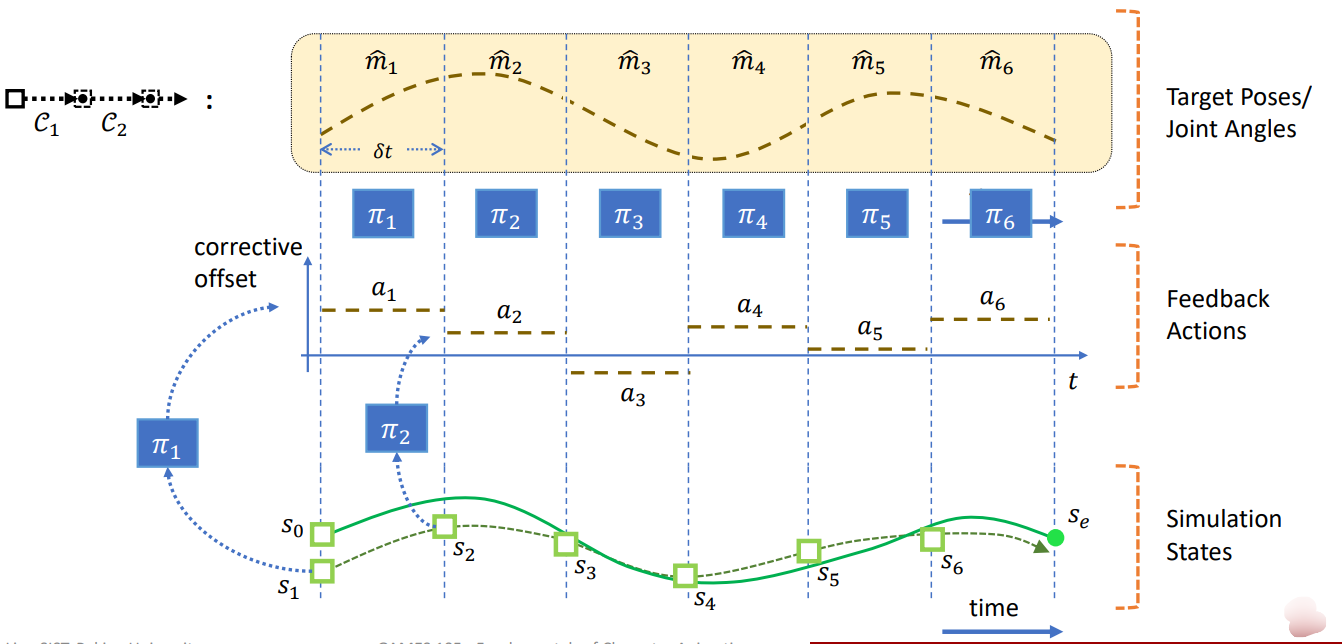
\includegraphics[totalheight=1.6in]{"./image/Feedback-Control.png"}
  \caption{Feedback Control} \label{fig:Feedback-Controll}
\end{figure}
反馈控制也能描述成轨迹优化的形式,区别在于:轨迹优化优化的是每一时刻的控制信号,但反馈控制
优化的是控制策略。控制本身是一个函数,可以由该函数,根据角色当前的状态,来计算一个控制信号。

不管是轨迹优化(开环控制),还是反馈控制,都属于最优控制的几种不同类型。区别可由图\ref{fig:OptimalControl}
可见:
\begin{figure}[htbp]
  \centering
  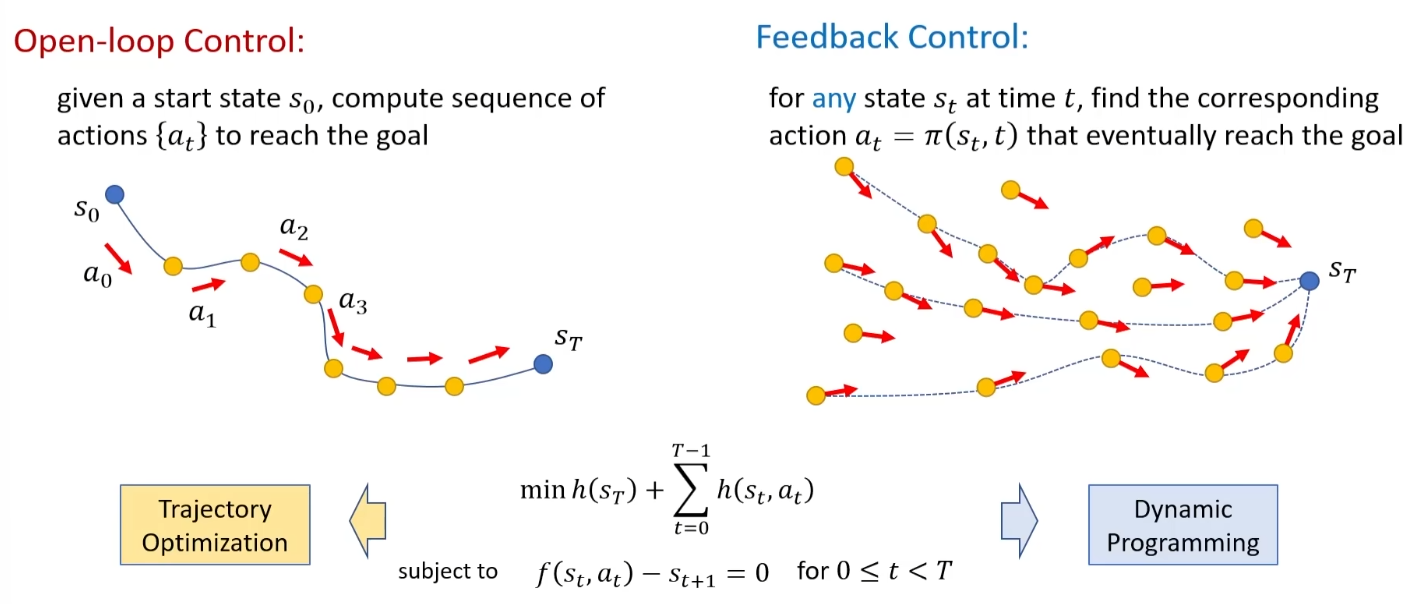
\includegraphics[totalheight=1.6in]{"./image/OptimalControl.png"}
  \caption{Optimal Control} \label{fig:OptimalControl}
\end{figure}
开环只需要知道起始点和目标点,好处是简单,坏处是禁不起扰动。反馈控制计算了状态空间中的所有状态,
更加困难,也更加使用,其理论基础来源于动态规划。

带约束的优化问题,除了前面讲的思路,还有经典的拉格朗日乘子法:对于目标函数$f(x)$
和限制条件$g(x)=0$其拉格朗日函数为:
\begin{equation}
  L(x, \lambda)=f(x)+\lambda^T g(x)
\end{equation}
拉格朗日解是原始问题的必要条件,因为解在目标函数和条件函数的梯度是平行关系。

优化目标\ref{eq:trajectory},\ref{eq:trajectorycontrol}的拉格朗日乘子函数有:
\begin{equation}
  L(s, a, \lambda)=h\left(s_T\right)+\sum_{t=0}^{T-1} h\left(s_t, a_t\right)+\lambda_{t+1}^T\left(f\left(s_t, a_t\right)-s_{t+1}\right)
\end{equation}
可以推出:
\begin{equation}
  \begin{aligned}
  \frac{\partial L}{\partial s_T} & =\frac{d h}{d s}\left(s_T\right)-\lambda_T=0 \\
  \frac{\partial L}{\partial s_t} & =\frac{\partial h}{\partial s}\left(s_t, a_t\right)+\left(\frac{\partial f}{\partial s}\left(s_t, a_t\right)\right)^T \lambda_{t+1}-\lambda_t=0 \\
  \frac{\partial L}{\partial a_t} & =\frac{\partial h}{\partial a}\left(s_t, a_t\right)+\left(\frac{\partial f}{\partial a}\left(s_t, a_t\right)\right)^T \lambda_{t+1}=0 \\
  \frac{\partial L}{\partial \lambda_t} & =f\left(s_t, a_t\right)-s_{t+1}=0
  \end{aligned}
\end{equation}
整理一下,可得到:
\begin{equation}
  \label{eq:PMP}
  \begin{array}{r}
    s_{t+1}=f\left(s_t, a_t\right) \\
  \text {"costate" dynamics } \quad \lambda_T=h_s^{\prime}\left(s_T\right) \\
  \lambda_t=h_s^{\prime}\left(s_t, a_t\right)+\left(f_s^{\prime}\left(s_t, a_t\right)\right)^T \lambda_{t+1} \\
  a_t=\arg \min _a h_a^{\prime}\left(s_t, a_t\right)+\left(f_a^{\prime}\left(s_t, a_t\right)\right)^T \lambda_{t+1}
  \end{array}
\end{equation}
方程\ref{eq:PMP}称为Pontryagin’s Maximum Principle(PMP)。在最优控制理论中,
开环控制最优的必要条件即为PMP。

PMP方程,最早是研发控制火箭而提出的方程,对于比较简单的系统分析起来比较方便。
PMP方程主要由一个前向过程+两个反向过程+一个更新过程。分别对应到方程中
$\{1\},\{2,3\},\{4\}$式子,最终优化出一个满足目标的轨迹$\{a_t\}$。


对于闭环控制,见\ref{fig:OptimalControl}右侧,可以从一个简单的例子来考虑这个问题:
找最短路径。 
\begin{figure}[htbp]
  \centering
  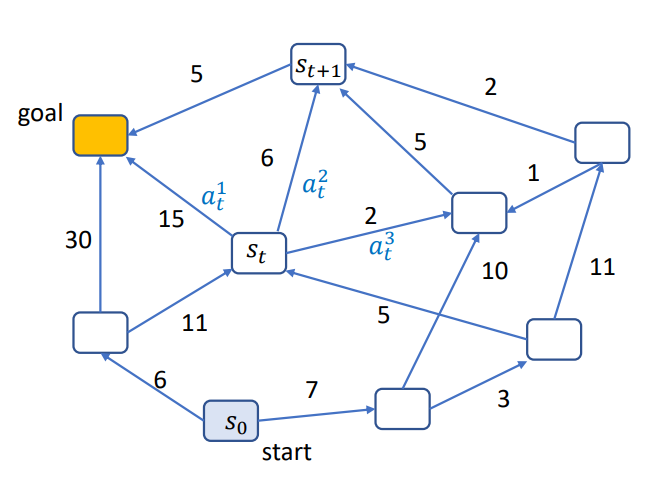
\includegraphics[totalheight=1.6in]{"./image/DynamicProgramming.png"}
  \caption{Dynamic Programming mini path} \label{fig:DynamicProgramming}
\end{figure}
找到一个策略$a_t = \pi(s_t)$,最小化$J(s_0) = \sum_{t=0}h(s_t, a_t)$,并且有
$s_{t+1}=f(s_t, a_t)$。
对于图\ref{fig:DynamicProgramming}中,可以将$a_t$理解为信号,$s_t$理解为状态。

问题:什么条件下,$\pi$是最优策略?答案是Bellman’s Principle。它告诉我们,
最优策略$\pi$,对于任何子问题,所给出的策略,也是最优的(动态规划中的最优子结构)。

从Bellman’s Principle出发,定义价值函数$V(s_i)$,表示从状态$s_i ^{j}$出发,到
目标位置,在最优策略$\pi(s_t)$下,得到的轨迹中所有边的代价和。
\begin{figure}[htbp]
  \centering
  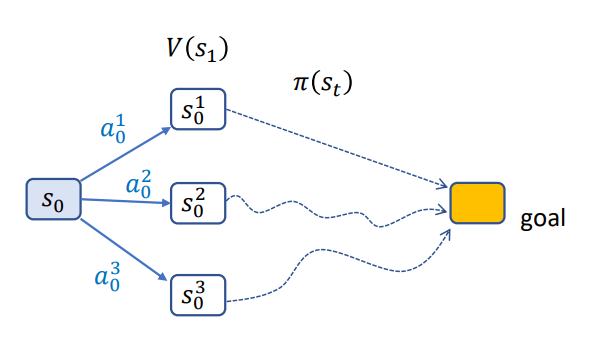
\includegraphics[totalheight=1.6in]{"./image/BellmanPrinciple.png"}
  \caption{Bellman Principle} \label{fig:BellmanPrinciple}
\end{figure}
假设我们得到了节点的价值函数,对于图\ref{fig:BellmanPrinciple}来说,
图中各节点数字均得到,根据最优子结构性质,要找到整体的最优策略,
只需要计算$a^{j}_0 + s^{j}_0$,哪一条最小,即可得到答案。也即知道价值函数
后,只需要计算上一时刻到当前时刻的代价加上当前时刻的价值函数,选出最小的,即为
最佳策略。

对于\ref{fig:DynamicProgramming}给定的符号,价值函数可以定义为:
\begin{equation}
  \begin{aligned}
  V\left(s_0\right) & =\min _\pi \sum_{t=0} h\left(s_t, a_t\right) \\
  \quad= & \min _{a_0}\left(h\left(s_0, a_0\right)+\min _\pi \sum_{t=1} h\left(s_t, a_t\right)\right)
  \end{aligned}
\end{equation}
简写形式被称为Belleman 方程:
\begin{equation}
  \label{eq:Belleman}
  V(s)=\min _a(h(s, a)+V(f(s, a)))
\end{equation}
它递归得给出了最优策略和价值函数的关系。同时,若得到了价值函数,
那么最优策略可以通过$\pi(s)=\arg \min _a(h(s, a)+V(f(s, a)))$
计算出来。也可以将$h(s, a)+V(f(s, a))$记为$Q(s,a)$,称为$Q$function,
或状态价值函数。

对于离散控制,优化$V$或$Q$问题不大,对于连续情况,比如人体运动所施加的力,
优化就可能变得很困难。

\subsection{LQR}
对于一般问题,Belleman方程可能没有解析解,而对于特定的问题,比如Linear Quadratic Regulator(LQR)
就有解析解。LQR要求目标函数$\min h\left(s_T\right)+\sum_{t=0}^{T-1} h\left(s_t, a_t\right)$中的$h$是一个二次函数,
对于运动学方程$f(s_t, a_t) - s_{t+1}=0$是一个线性函数。

在PD控制章节部分,给出的例子\ref{fig:PDController},就是一个典型的LQR问题。假设我们的目标轨迹是一个
正弦函数,则优化目标可写为:
\begin{equation}
  \begin{aligned}
  & \min _{\left\{x_n, v_n, \bar{x}_n\right\}} \sum_{n=0}^N\left(\sin \left(t_n\right)-x_n\right)^2+\sum_{n=0}^N \bar{x}_n^2 \\
  & \text { s.t. } \quad \begin{aligned}
  v_{n+1} & =v_n+h\left(k_p\left(\bar{x}_n-x_n\right)-k_d v_n\right) \\
  & x_{n+1}=x_n+h v_{n+1}
  \end{aligned}
  \end{aligned}
\end{equation}

对于一般LQR问题,优化目标可写为:
\begin{equation}
  \begin{aligned}
  & \qquad \min s_T^T Q_T s_T+\sum_{t=0}^T s_t^T Q_t s_t+a_t^T R_t a_t \\
  & \text {满足} \\
  & \qquad s_{t+1}=A_t s_t+B_t a_t \quad \text {其中} 0 \leq t<T
  \end{aligned}
\end{equation}
其目标函数是一个二次型,运动学方程中下一个运动状态等于上一个状态乘以一个矩阵
加上控制信号乘以一个矩阵。

结合贝尔曼方程和图\ref{fig:BellmanPrinciple},可以得到递归求解LQR问题的思路。
\begin{enumerate}
  \setlength{\itemindent}{2em}
  \item 计算最后一步得到$V\left(s_T\right)=\min _{a_T} s_T^T Q_T s_T=s_T^T Q_T S_T$
  \item 计算倒数第二步:$$
  \begin{aligned}
  Q\left(s_{T-1}, a_{T-1}\right) & =s_{T-1}^T\left(Q_{T-1}+A_{T-1}^T Q_T A_{T-1}\right) s_{T-1} \\
  & +a_{T-1}^T\left(R_{T-1}+B_{T-1}^T Q_T B_{T-1}\right) a_{T-1} \\
  & +2 s_{T-1}^T A_{T-1}^T Q_T B_{T-1} a_{T-1}
  \end{aligned}
  $$
  $$
\begin{aligned}
a_{T-1}^* & =\arg \min _{a_{T-1}} Q\left(s_{T-1}, a_{T-1}\right) \\
& =-\left(R_{T-1}+B_{T-1}^T Q_T B_{T-1}\right)^{-1} B_{T-1}^T Q_T A_{T-1} s_{T-1}
\end{aligned}
$$
  \item 记$K_{T-1}=\left(R_{T-1}+B_{T-1}^T Q_T B_{T-1}\right)^{-1} B_{T-1}^T Q_T A_{T-1}$,
  \item 计算中间第$T -i,1 < i \leq T$:
  $$
    \begin{aligned}
    & a_t^*=-K_t s_t \\
    & K_t=\left(R_t+B_t^T P_{t+1} B_t\right)^{-1} B_t^T P_{t+1} A_t \\
    & V\left(s_t\right)=s_t^T P_t s_t \\
    & P_t=F\left(P_{t+1}\right)=\cdots
    \end{aligned}
    $$
\end{enumerate}
看起来比较复杂,其实在第二步的时候,就看出了,$V(s_{T-1})$仍然
是个二次函数,并且形式上和$V_{s_T}$保持一致。

如何处理非线性运动方程的情况?比如人体,旋转部分就引入了非线性性。
如何处理目标函数非线性问题,而不是此处的二次型形式?一种思路是将非线性近似为线性。
比如泰勒展开(加速对应的函数都可高阶微分)。

目标函数的二阶近似:
\begin{equation}
  h\left(s_t, a_t\right) \approx h\left(\bar{s}_t, \bar{a}_t\right)+\nabla h\left(\bar{s}_t, \bar{a}_t\right)\left[\begin{array}{l}
  s_t-\bar{s}_t \\
  a_t-\bar{a}_t
  \end{array}\right]+\frac{1}{2}\left[\begin{array}{c}
  s_t-\bar{s}_t \\
  a_t-\bar{a}_t
  \end{array}\right]^T \nabla^2 h\left(\bar{s}_t, \bar{a}_t\right)\left[\begin{array}{l}
  s_t-\bar{s}_t \\
  a_t-\bar{a}_t
  \end{array}\right]
\end{equation}

运动方程的一阶近似:
\begin{equation}
  f\left(s_t, a_t\right) \approx f\left(\bar{s}_t, \bar{a}_t\right)+\nabla f\left(\bar{s}_t, \bar{a}_t\right)\left[\begin{array}{l}
  s_t-\bar{s}_t \\
  a_t-\bar{a}_t
  \end{array}\right]
\end{equation}
对应有称为迭代IQR(iterative IQR)的求解方法。

或者二阶近似:
\begin{equation}
  f\left(s_t, a_t\right) \approx * * *+\frac{1}{2}\left[\begin{array}{c}
  s_t-\bar{s}_t \\
  a_t-\bar{a}_t
  \end{array}\right]^T \nabla^2 f\left(\bar{s}_t, \bar{a}_t\right)\left[\begin{array}{l}
  s_t-\bar{s}_t \\
  a_t-\bar{a}_t
  \end{array}\right]
\end{equation}
对应有称为DDP(Differential Dynamic Programming)的求解方法。

\section{不基于模型的方法}
前面讲的最优控制,都是假设运动方程是知道的,否则推到无法展开。
这种方法被称为基于模型的方法。基于模型的方法弊端不言而喻,
实际工作中,往往是不知道具体的模型函数的,设计出来,往往也缺乏精度。
比如碰撞模拟,都是对真实碰撞的一种不精确建模。
另外,如果系统有噪音,比如对真实世界中的机器人,测量出来的
数据有很大误差,硬件采集也有噪音等,最后系统高度非线性的时候,算出来的梯度都不可靠。
总的来说,对于复杂的系统,基于模型的方法,是难以实用的。

不基于模型的方法,并不是对模型一无所知,只是模型比较复杂,难以给出来,
主要是在给定优化函数下,利用基于模型的方式,对中间过程做优化建模,最后优化目标函数。
具体由有基于采样的,基于强化学习的方法。

\subsection{基于采样的优化}
% 迭代方法:
% \begin{enumerate}
%   \item 
% \end{enumerate}

\begin{figure}[htbp]
  \centering
  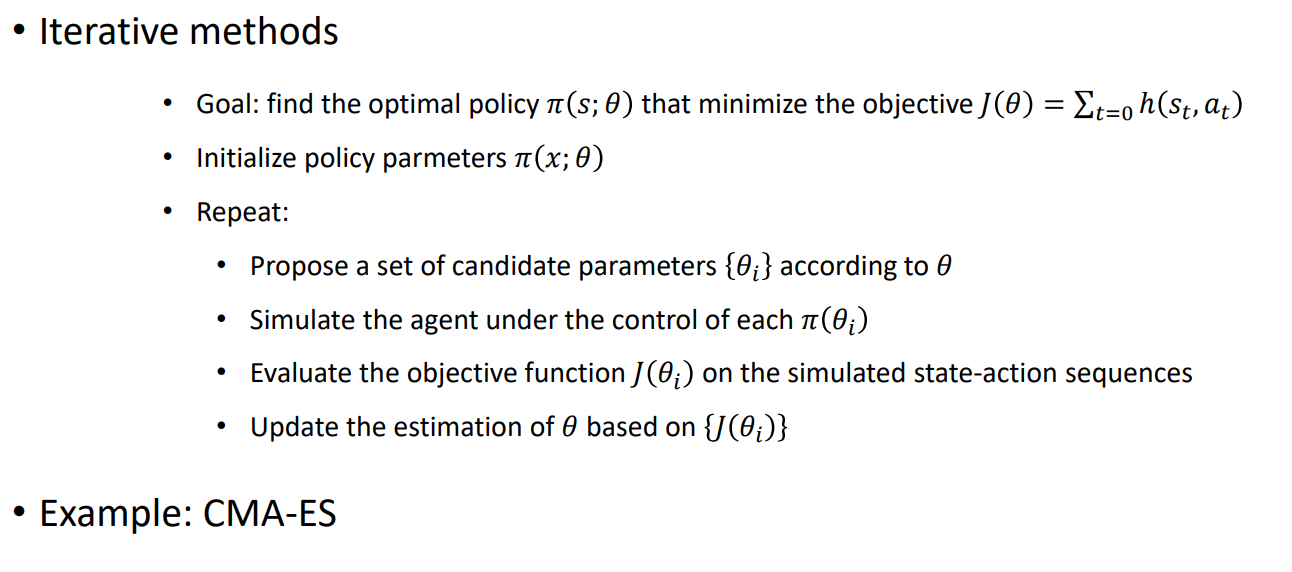
\includegraphics[totalheight=1.6in]{"./image/SamplingbasedPolicyOptimization.png"}
  \caption{Sampling based Policy Optimization} \label{fig:SamplingbasedPO}
\end{figure}

两个例子:
\begin{enumerate}
  \setlength{\itemindent}{2em}
  \item CMA-ES
  \item Liu et al. 2012 – Terrain Runner
\end{enumerate}

具体略。

\subsection{强化学习}
强化学习和最优控制差不多具有相同的优化目标。
\begin{equation}
  \max \sum_{t=0} r\left(s_t, a_t\right)
\end{equation}
但是强化学习不需要对系统做精确的假设,比如最优控制需要满足
运动方程。$f(s_t, a_t) - s_{t+1}=0$,强化学习(RL)不需要这样。
它完全由系统同世界的交互,通过采样,来更新,取得极值。
虽然要求对系统有比较准确的描述,但还是可以利用模型,来提高优化效率。
这种模型也不一定是真的模型,而是可以从数据中学到一个模型,来指导RL的
优化。

\subsubsection{马尔可夫决策过程和贝尔曼方程}
RL实际上是在求解一个马尔可夫决策过程(MDP)。

MDP实际上是一个离散时间随机控制过程,它与世界交互的方式和具体数学描述
见\ref{fig:MDP},也可参考\href{https://github.com/foocker/RL}{RL}。
\begin{figure}[htbp]
  \centering
  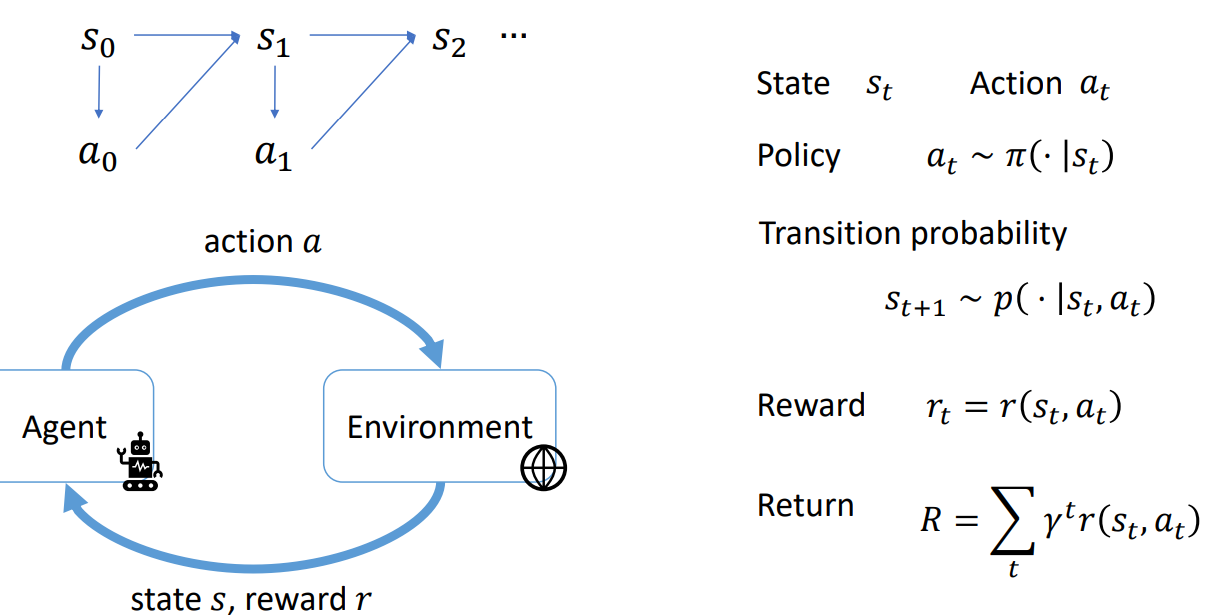
\includegraphics[totalheight=2in]{"./image/MDP.png"}
  \caption{Markov Decision Process} \label{fig:MDP}
\end{figure}
具有马尔可夫性。一个MDP问题具有如下数学形式:
对于给定空间
\begin{equation}
  \mathcal{M}=\{S, A, p, r\}
\end{equation}
求解一个策略$\pi(a|s)$的最优化期望回报$J$,
\begin{equation}
  J=E[R]=E_{\tau \sim \pi}\left[\sum_t \gamma^t r\left(s_t, a_t\right)\right]
\end{equation}
在由$\pi$得出的所有轨迹$\tau=\left\{s_0, a_0, s_1, a_1, \ldots\right\}$中计算期望。

在最优控制中是直接优化最优方程,这里因为策略$\pi$有大量噪音,导致状态是随着概率在变化。
因此定义为在所有状态下的所有return的期望值。

把一个跟踪问题(轨迹优化问题)变成一个MDP问题。在Reward函数中,将
参考数据和仿真数据做一个差,最后在轨迹上求和,即可。

对比最优控制和强化控制。
在最优控制中:
\begin{enumerate}
  \setlength{\itemindent}{2em}
  \item 价值函数:$V(s)=\min _a(h(s, a)+V(f(s, a)))$
  \item 最优策略:$\pi(s)=\arg \min _a(h(s, a)+V(f(s, a)))$
  \item 最优Q函数:$Q(s, a)=h(s, a)+V(f(s, a))$
\end{enumerate}

在RL控制中:
\begin{enumerate}
  \setlength{\itemindent}{2em}
  \item 策略的价值函数:$V^\pi(s)=E_{\tau \sim \pi}\left[r(s, a)+V\left(s^{\prime}\right)\right]$
  \item 策略的Q函数:$Q^\pi(s, a)=r(s, a)+E_{\tau \sim \pi}\left[V\left(s^{\prime}\right)\right]$
\end{enumerate}
对于离散的RL问题,也可以像最优控制中那样求解,但对于连续的问题,只能如上中求解。
其中策略价值函数不需要一定最优。

求解基于价值方法的MDP问题:
\begin{enumerate}
  \setlength{\itemindent}{2em}
  \item 利用贝尔曼方程去学习价值函数或者Q函数
  \item 利用求得的Q函数估计策略(状态关于动作的最小值)
  \item 主要用在离散问题上,比如Q-learning,DQN(2015)
\end{enumerate}

基于Value function的方法,比如DQN,要求控制空间必须离散,状态空间可以连续。
将它用在角色控制上,比如玩滑板,当玩家在撞到物体时,需要切换到另一个状态,若控制是连续的,
则只能摔倒。

强化学习的另外一类方法,Policy Gradient。
\begin{enumerate}
  \setlength{\itemindent}{2em}
  \item 利用贝尔曼方程去学习价值函数或者Q函数
  \item 利用Monte-Carlo方法近似逼近价值函数的策略梯度(不可导,在推导过程中利用统计的技巧将不可导部分消去,使得能计算梯度)
  \item 利用策略梯度更新策略
  \item 对连续问题比较合适,比如REIBFORCE,TRPO,PPO等
\end{enumerate}
控制策略是显式定义的,因此不需要去求解优化问题,找到下一个action,
而只需要对策略(Policy)进行求值,就可以得到需要的action。因此对连续问题
比较有效。

PPO在物理角色动画中用得非常广泛。使用RL加上一点轨迹优化,就可以实现非常复杂的动作控制。
比如如下工作:
\begin{enumerate}
  \setlength{\itemindent}{2em}
  \item Liu et al. 2016. ControlGraphs
  \item Peng et al. 2018. DeepMimic
\end{enumerate}

除此之外,还有另外Policy Gradient和Value Based方法结合,
被称为Actor Critic方法。

生成控制策略,可以由生成模型VAE,GAN,SD等结合RL来实现物理角色动画,需要把控制策略换成
生成网络。不过RL的问题在于不稳定。

\section{展望}
生成可控的,基于物理的动画,可以用来代替基于关键帧的方法,基于运动学的方法。因为运动控制的难度,
可编辑的难度,风格化的难度,都带来了很大的实际应用的挑战。不过按目前的发展情况来看,还是有希望的。

大规模预训练模型,这个在ChatGPT中已经有初步验证。针对大规模的运动控制数据,学习一个大规模的运动控制
模型,类似于小脑的功能。

数字演员,人群运动控制。

\begin{figure}[htbp]
  \centering
  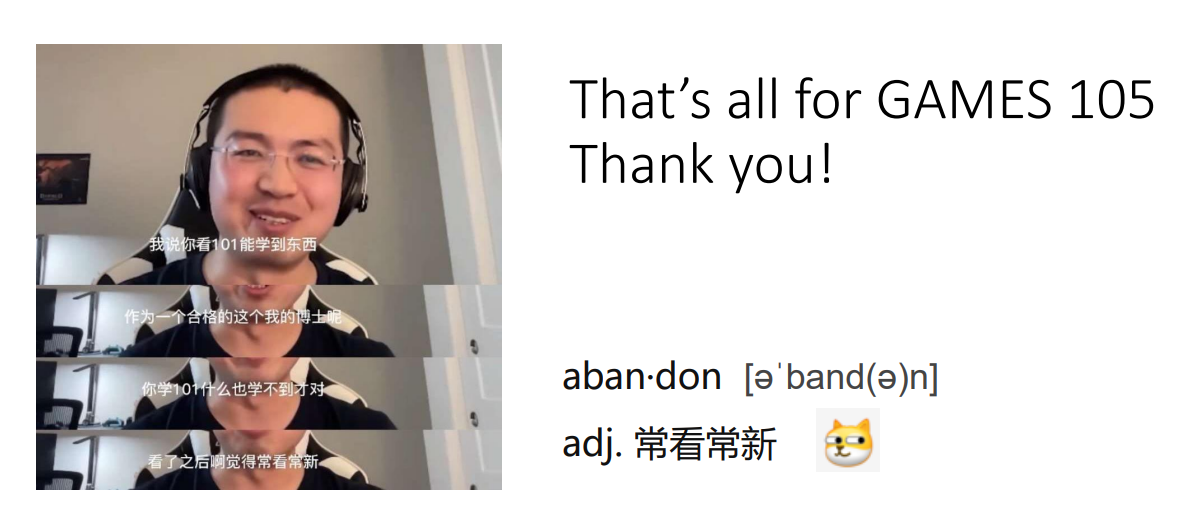
\includegraphics[totalheight=2in]{"./image/games105.png"}
  \caption{games105} \label{fig:games105}
\end{figure}

\newpage
\begin{problemset}
  \item 完成一个RL与动作控制的开源项目
\end{problemset}

\chapter{ElegantBook 写作示例}

\begin{introduction}
  \item 积分定义~\ref{def:int}
  \item Fubini 定理~\ref{thm:fubi}
  \item 最优性原理~\ref{pro:max}
  \item 柯西列性质~\ref{property:cauchy}
  \item 韦达定理
\end{introduction}

\section{Lebesgue 积分}
在前面各章做了必要的准备后,本章开始介绍新的积分。在 Lebesgue 测度理论的基础上建立了 Lebesgue 积分,其被积函数和积分域更一般,可以对有界函数和无界函数统一处理。正是由于 Lebesgue 积分的这些特点,使得 Lebesgue 积分比 Riemann 积分具有在更一般条件下的极限定理和累次积分交换积分顺序的定理,这使得 Lebesgue 积分不仅在理论上更完善,而且在计算上更灵活有效。

Lebesgue 积分有几种不同的定义方式。我们将采用逐步定义非负简单函数,非负可测函数和一般可测函数积分的方式。

由于现代数学的许多分支如概率论、泛函分析、调和分析等常常用到一般空间上的测度与积分理论,在本章最后一节将介绍一般的测度空间上的积分。

\subsection{积分的定义}

我们将通过三个步骤定义可测函数的积分。首先定义非负简单函数的积分。以下设 $E$ 是 $\mathcal{R}^n$ 中的可测集。

\begin{definition}[可积性] \label{def:int} 
设 $ f(x)=\sum\limits_{i=1}^{k} a_i \chi_{A_i}(x)$ 是 $E$ 上的\textbf{非负简单函数},中文其中 $\{A_1,A_2,\ldots,A_k\}$ 是 $E$ 上的一个可测分割,$a_1,a_2,\ldots,a_k$ 是非负实数。定义 $f$ 在 $E$ 上的积分为 $\int_{a}^b f(x)$
\begin{equation}
   \label{inter}
   \int_{E} f dx = \sum_{i=1}^k a_i m(A_i) \pi \alpha\beta\sigma\gamma\nu\xi\epsilon\varepsilon. \oint_{a}^b\ointop_{a}^b\prod_{i=1}^n
\end{equation}
一般情况下 $0 \leq \int_{E} f dx \leq \infty$。若 $\int_{E} f dx < \infty$,则称 $f$ 在 $E$ 上可积。
\end{definition}

一个自然的问题是,Lebesgue 积分与我们所熟悉的 Riemann 积分有什么联系和区别?在 4.4 在我们将详细讨论 Riemann 积分与 Lebesgue 积分的关系。这里只看一个简单的例子。设 $D(x)$ 是区间 $[0,1]$ 上的 Dirichlet 函数。即 $D(x)=\chi_{Q_0}(x)$,其中 $Q_0$ 表示 $[0,1]$ 中的有理数的全体。根据非负简单函数积分的定义,$D(x)$ 在 $[0,1]$ 上的 Lebesgue 积分为
\begin{equation}
   \label{inter2}
   \int_0^1 D(x)dx = \int_0^1 \chi_{Q_0} (x) dx = m(Q_0) = 0
\end{equation}
即 $D(x)$ 在 $[0,1]$ 上是 Lebesgue 可积的并且积分值为零。但 $D(x)$ 在 $[0,1]$ 上不是 Riemann 可积的。


有界变差函数是与单调函数有密切联系的一类函数。有界变差函数可以表示为两个单调递增函数之差。与单调函数一样,有界变差函数几乎处处可导。与单调函数不同,有界变差函数类对线性运算是封闭的,它们构成一线空间。练习题 \ref{exer:43} 是一个性质的证明。

\begin{exercise}\label{exer:43}
设 $f \notin\in L(\mathcal{R}^1)$,$g$ 是 $\mathcal{R}^1$ 上的有界可测函数。证明函数
\begin{equation}
   \label{ex:1}
   I(t) = \int_{\mathcal{R}^1} f(x+t)g(x)dx \quad t \in \mathcal{R}^1
\end{equation}
是 $\mathcal{R}^1$ 上的连续函数。 
\end{exercise}

\begin{solution}
即 $D(x)$ 在 $[0,1]$ 上是 Lebesgue 可积的并且积分值为零。但 $D(x)$ 在 $[0,1]$ 上不是 Riemann 可积的。
\end{solution}

\begin{proof}
即 $D(x)$ 在 $[0,1]$ 上是 Lebesgue 可积的并且积分值为零。但 $D(x)$ 在 $[0,1]$ 上不是 Riemann 可积的。
\end{proof}

\begin{theorem}[Fubini 定理] \label{thm:fubi} 
(1)若 $f(x,y)$ 是 $\mathcal{R}^p\times\mathcal{R}^q$ 上的非负可测函数,则对几乎处处的 $x\in \mathcal{R}^p$,$f(x,y)$ 作为 $y$ 的函数是 $\mathcal{R}^q$ 上的非负可测函数,$g(x)=\int_{\mathcal{R}^q}f(x,y) dy$ 是 $\mathcal{R}^p$ 上的非负可测函数。并且
\begin{equation}
   \label{eq:461}
   \int_{\mathcal{R}^p\times\mathcal{R}^q} f(x,y) dxdy=\int_{\mathcal{R}^p}\left(\int_{\mathcal{R}^q}f(x,y)dy\right)dx.
\end{equation}

(2)若 $f(x,y)$ 是 $\mathcal{R}^p\times\mathcal{R}^q$ 上的可积函数,则对几乎处处的 $x\in\mathcal{R}^p$,$f(x,y)$ 作为 $y$ 的函数是 $\mathcal{R}^q$ 上的可积函数,并且 $g(x)=\int_{\mathcal{R}^q}f(x,y) dy$ 是 $\mathcal{R}^p$ 上的可积函数。而且~\eqref{eq:461} 成立。
\end{theorem}

\begin{note}
在本模板中,引理(lemma),推论(corollary)的样式和定理~\ref{thm:fubi} 的样式一致,包括颜色,仅仅只有计数器的设置不一样。
\end{note}

我们说一个实变或者复变量的实值或者复值函数是在区间上平方可积的,如果其绝对值的平方在该区间上的积分是有限的。所有在勒贝格积分意义下平方可积的可测函数构成一个希尔伯特空间,也就是所谓的 $L^2$ 空间,几乎处处相等的函数归为同一等价类。形式上,$L^2$ 是平方可积函数的空间和几乎处处为 0 的函数空间的商空间。

\begin{proposition}[最优性原理] \label{pro:max}
如果 $u^*$ 在 $[s,T]$ 上为最优解,则 $u^*$ 在 $[s, T]$ 任意子区间都是最优解,假设区间为 $[t_0, t_1]$ 的最优解为 $u^*$ ,则 $u(t_0)=u^{*}(t_0)$,即初始条件必须还是在 $u^*$ 上。
\end{proposition}

我们知道最小二乘法可以用来处理一组数据,可以从一组测定的数据中寻求变量之间的依赖关系,这种函数关系称为经验公式。本课题将介绍最小二乘法的精确定义及如何寻求点与点之间近似成线性关系时的经验公式。假定实验测得变量之间的 $n$ 个数据,则在平面上,可以得到 $n$ 个点,这种图形称为 “散点图”,从图中可以粗略看出这些点大致散落在某直线近旁, 我们认为其近似为一线性函数,下面介绍求解步骤。

\begin{figure}[htbp]
  \centering
  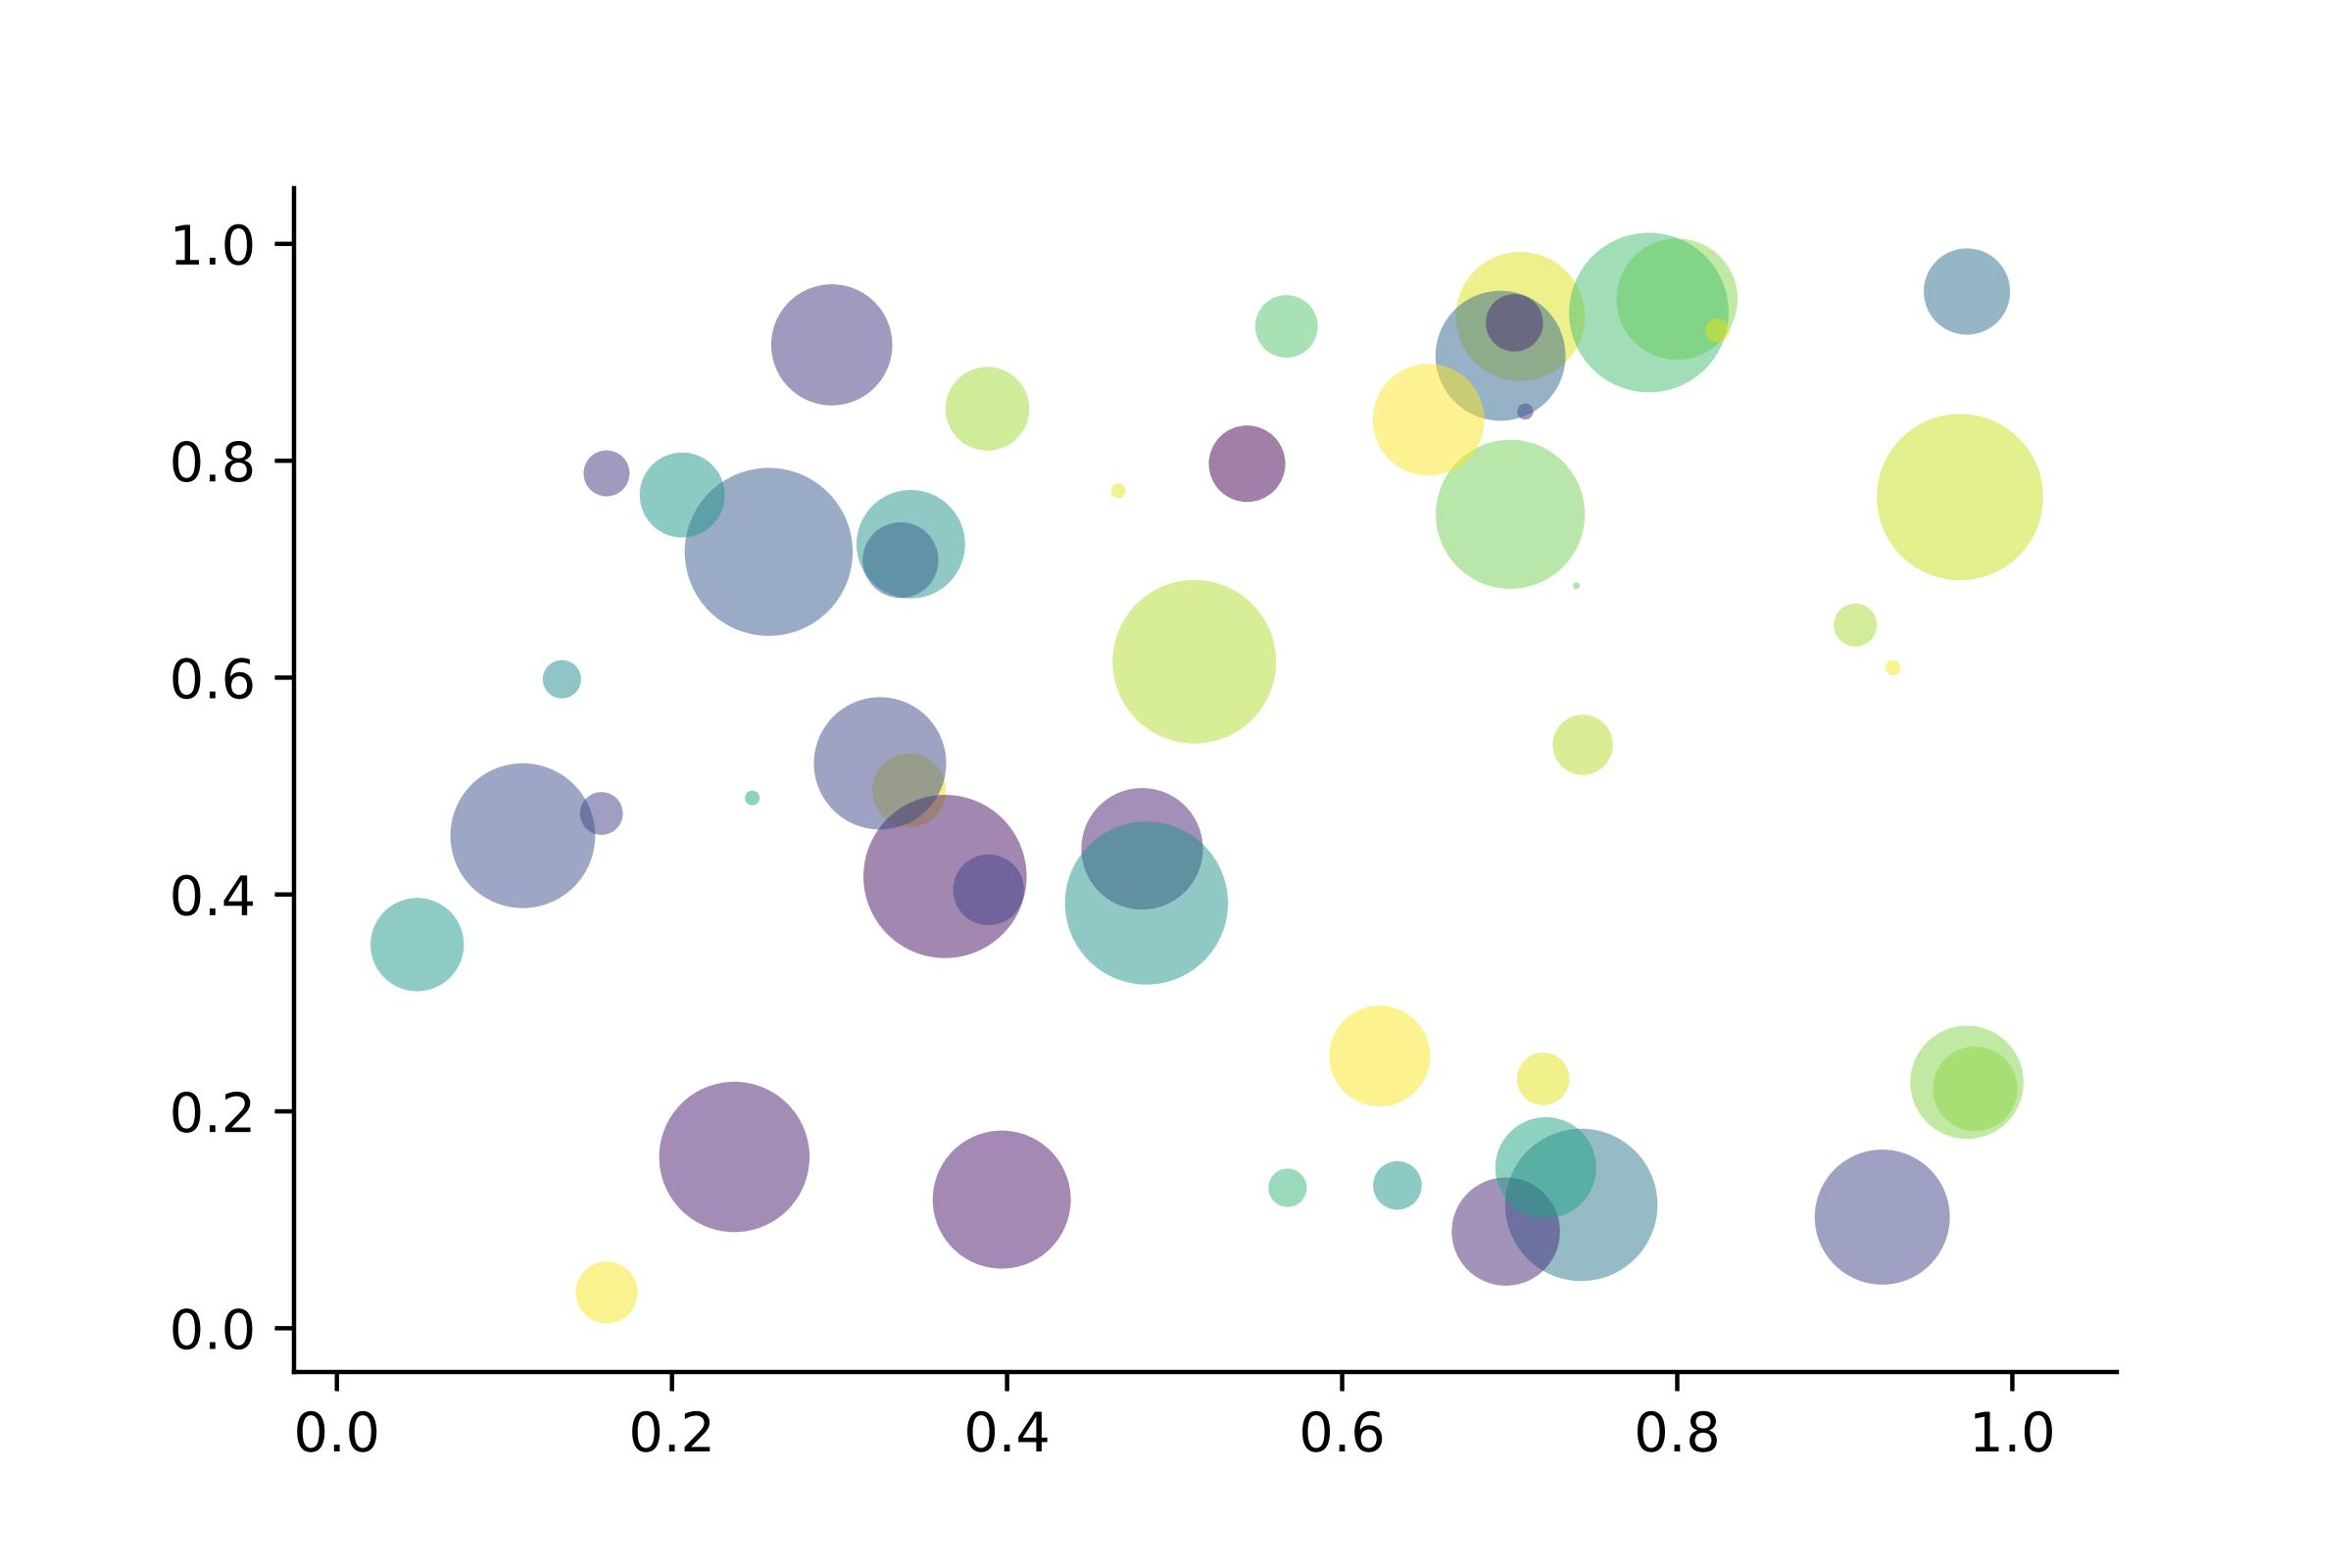
\includegraphics[width=0.6\textwidth]{scatter.jpg}
  \caption{散点图示例 $\hat{y}=a+bx$ \label{fig:scatter}}
\end{figure}

以最简单的一元线性模型来解释最小二乘法。什么是一元线性模型呢?监督学习中,如果预测的变量是离散的,我们称其为分类(如决策树,支持向量机等),如果预测的变量是连续的,我们称其为回归。回归分析中,如果只包括一个自变量和一个因变量,且二者的关系可用一条直线近似表示,这种回归分析称为一元线性回归分析。如果回归分析中包括两个或两个以上的自变量,且因变量和自变量之间是线性关系,则称为多元线性回归分析。对于二维空间线性是一条直线;对于三维空间线性是一个平面,对于多维空间线性是一个超平面。

\begin{property}\label{property:cauchy}
柯西列的性质
\begin{enumerate}
\item $\{x_k\}$ 是柯西列,则其子列 $\{x_k^i\}$ 也是柯西列。
\item $x_k\in \mathcal{R}^n$,$\rho(x,y)$ 是欧几里得空间,则柯西列收敛,$(\mathcal{R}^n,\rho)$ 空间是完备的。
\end{enumerate}
\end{property}

\begin{conclusion}
回归分析(regression analysis) 是确定两种或两种以上变量间相互依赖的定量关系的一种统计分析方法。运用十分广泛,回归分析按照涉及的变量的多少,分为一元回归和多元回归分析;按照因变量的多少,可分为简单回归分析和多重回归分析;按照自变量和因变量之间的关系类型,可分为线性回归分析和非线性回归分析。
\end{conclusion}

\begin{problemset}
\item 设 $A$ 为数域 $K$ 上的 $n$ 级矩阵。证明:如果 $K^n$ 中任意非零列向量都是 $A$ 的特征向量,则 $A$ 一定是数量矩阵。
\item 证明:不为零矩阵的幂零矩阵不能对角化。
\item 设 $A = (a_{ij})$ 是数域 $K$ 上的一个 $n$ 级上三角矩阵,证明:如果 $a_{11} = a_{22} = \cdots = a_{nn}$,并且至少有一个 $a_{kl} \not = 0 (k < l)$,则 $A$ 一定不能对角化。
\end{problemset}


\nocite{*}
\printbibliography[heading=bibintoc, title=\ebibname]
\appendix

\chapter{基本数学工具}


本附录包括了计量经济学中用到的一些基本数学,我们扼要论述了求和算子的各种性质,研究了线性和某些非线性方程的性质,并复习了比例和百分数。我们还介绍了一些在应用计量经济学中常见的特殊函数,包括二次函数和自然对数,前 4 节只要求基本的代数技巧,第 5 节则对微分学进行了简要回顾;虽然要理解本书的大部分内容,微积分并非必需,但在一些章末附录和第 3 篇某些高深专题中,我们还是用到了微积分。

\section{求和算子与描述统计量}

\textbf{求和算子} 是用以表达多个数求和运算的一个缩略符号,它在统计学和计量经济学分析中扮演着重要作用。如果 $\{x_i: i=1, 2, \ldots, n\}$ 表示 $n$ 个数的一个序列,那么我们就把这 $n$ 个数的和写为:

\begin{equation}
\sum_{i=1}^n x_i \equiv x_1 + x_2 +\cdots + x_n
\end{equation}

\end{document}
